\begin{appendices}

    % -------------------------------
    % -------------------------------
    % ------- BAYSIS Appendix -------
    % -------------------------------
    % -------------------------------
    \chapter{BAYSIS Figures, Tables and Listings}
    \label{appendix_baysis}
    
    % --------------------------------
    % ------- BAYSIS Dataset ---------
    % --------------------------------
    % \tocless\section{BAYSIS Data Foundation}
    % \label{appendix_baysis_dataset}
    
    % ------- BAYSIS Dataset - Figures --------
    \begin{figure}[ht!]
        \centering
        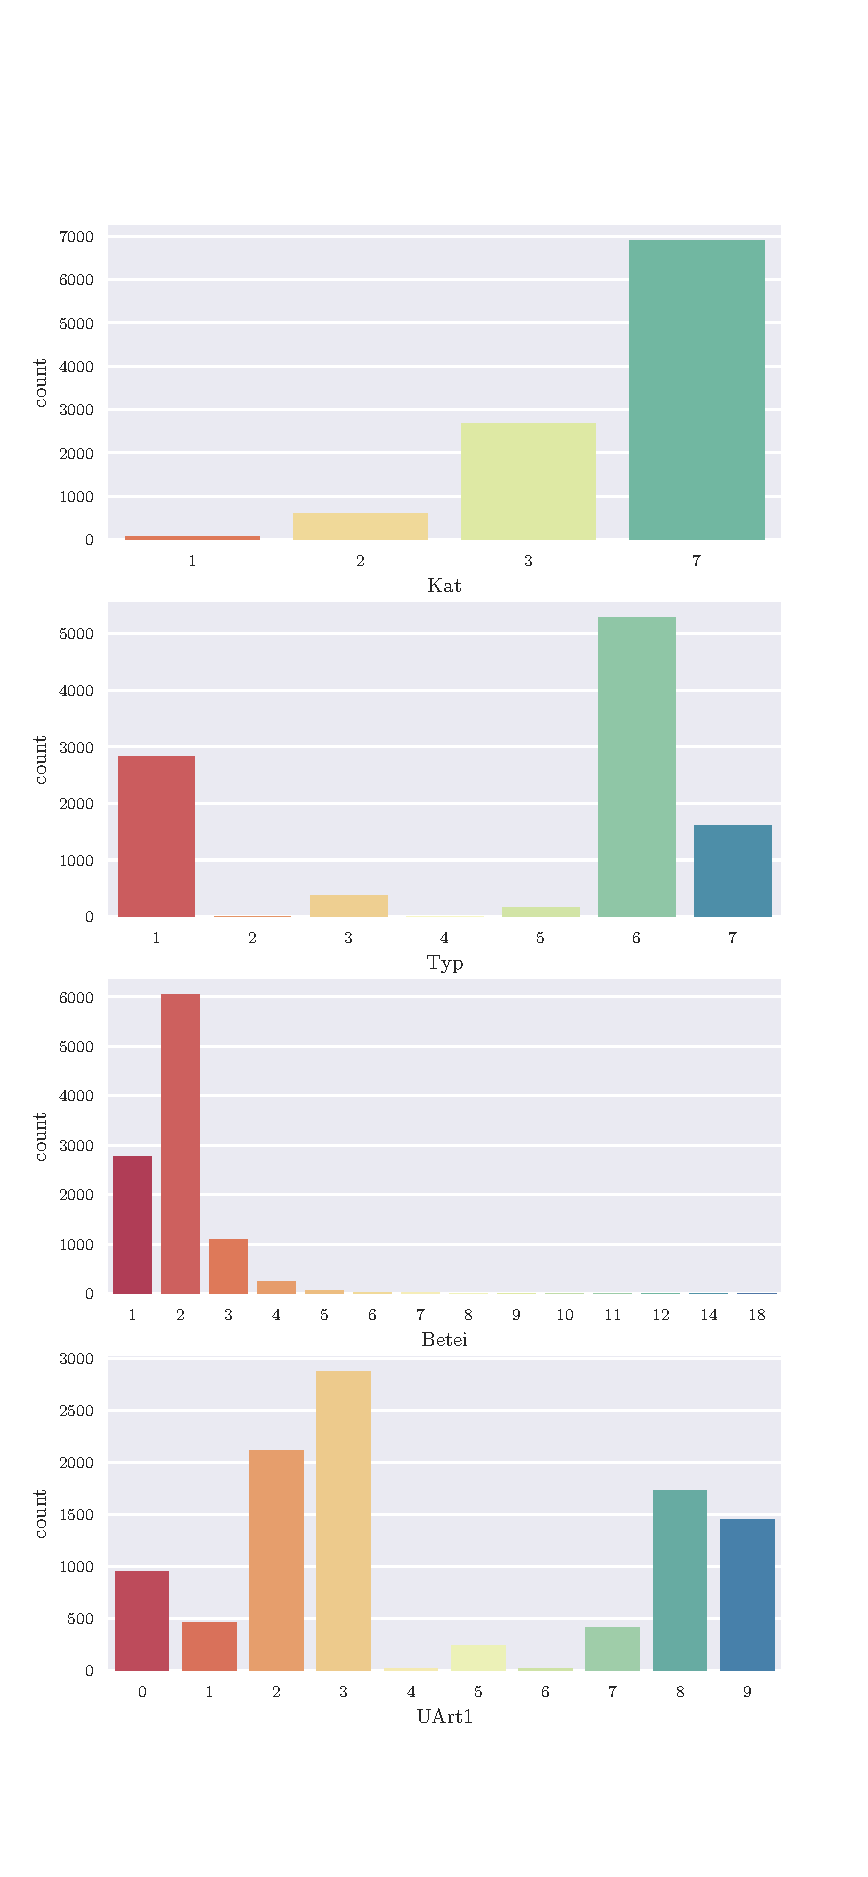
\includegraphics[scale=0.7]{CorrAnalysis/data/BAYSIS/01_dataset/plots/baysis_dataset_count_multiple01}
        \caption{Distribution of the accident category Kat, Typ, Betei and UArt}
        \label{img:baysis_dataset_Kat}
        \label{img:baysis_dataset_Typ}
        \label{img:baysis_dataset_Betei}
        \label{img:baysis_dataset_UArt}
    \end{figure}

    \begin{figure}[ht!]
        \centering
        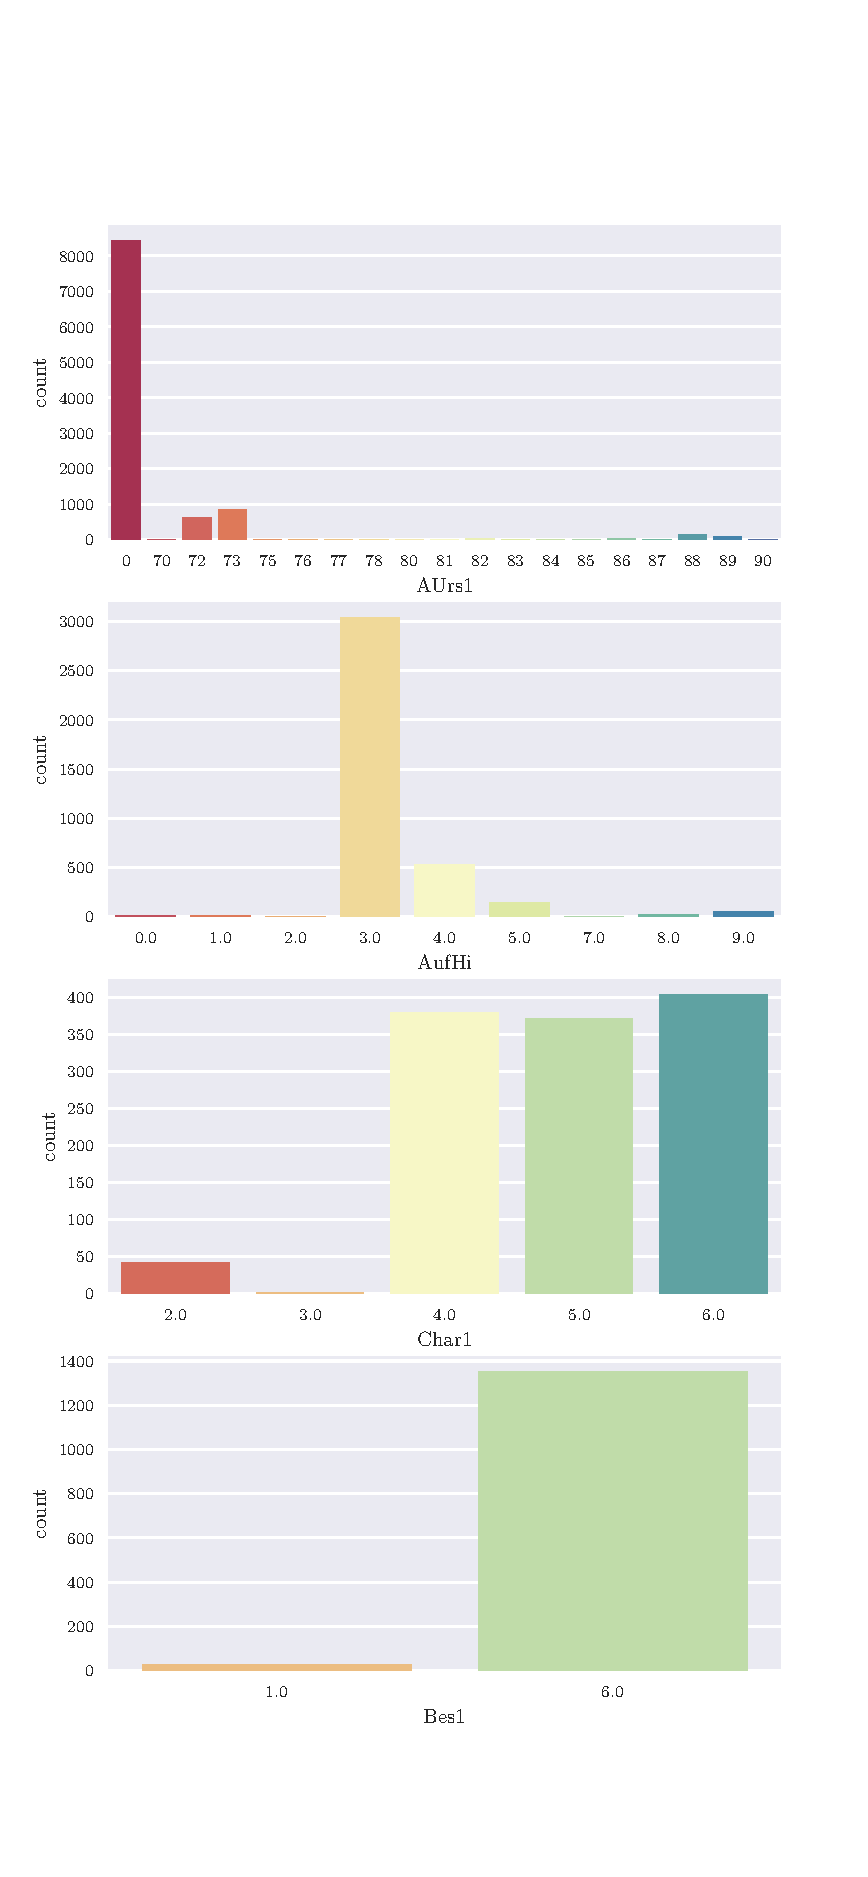
\includegraphics[scale=0.7]{CorrAnalysis/data/BAYSIS/01_dataset/plots/baysis_dataset_count_multiple02}
        \caption{Distribution of the accident category AUrs, AufHi, Char and Bes}
        \label{img:baysis_dataset_AUrs}
        \label{img:baysis_dataset_AufHi}
        \label{img:baysis_dataset_Char}
        \label{img:baysis_dataset_Bes}
    \end{figure}

    \begin{figure}[ht!]
        \centering
        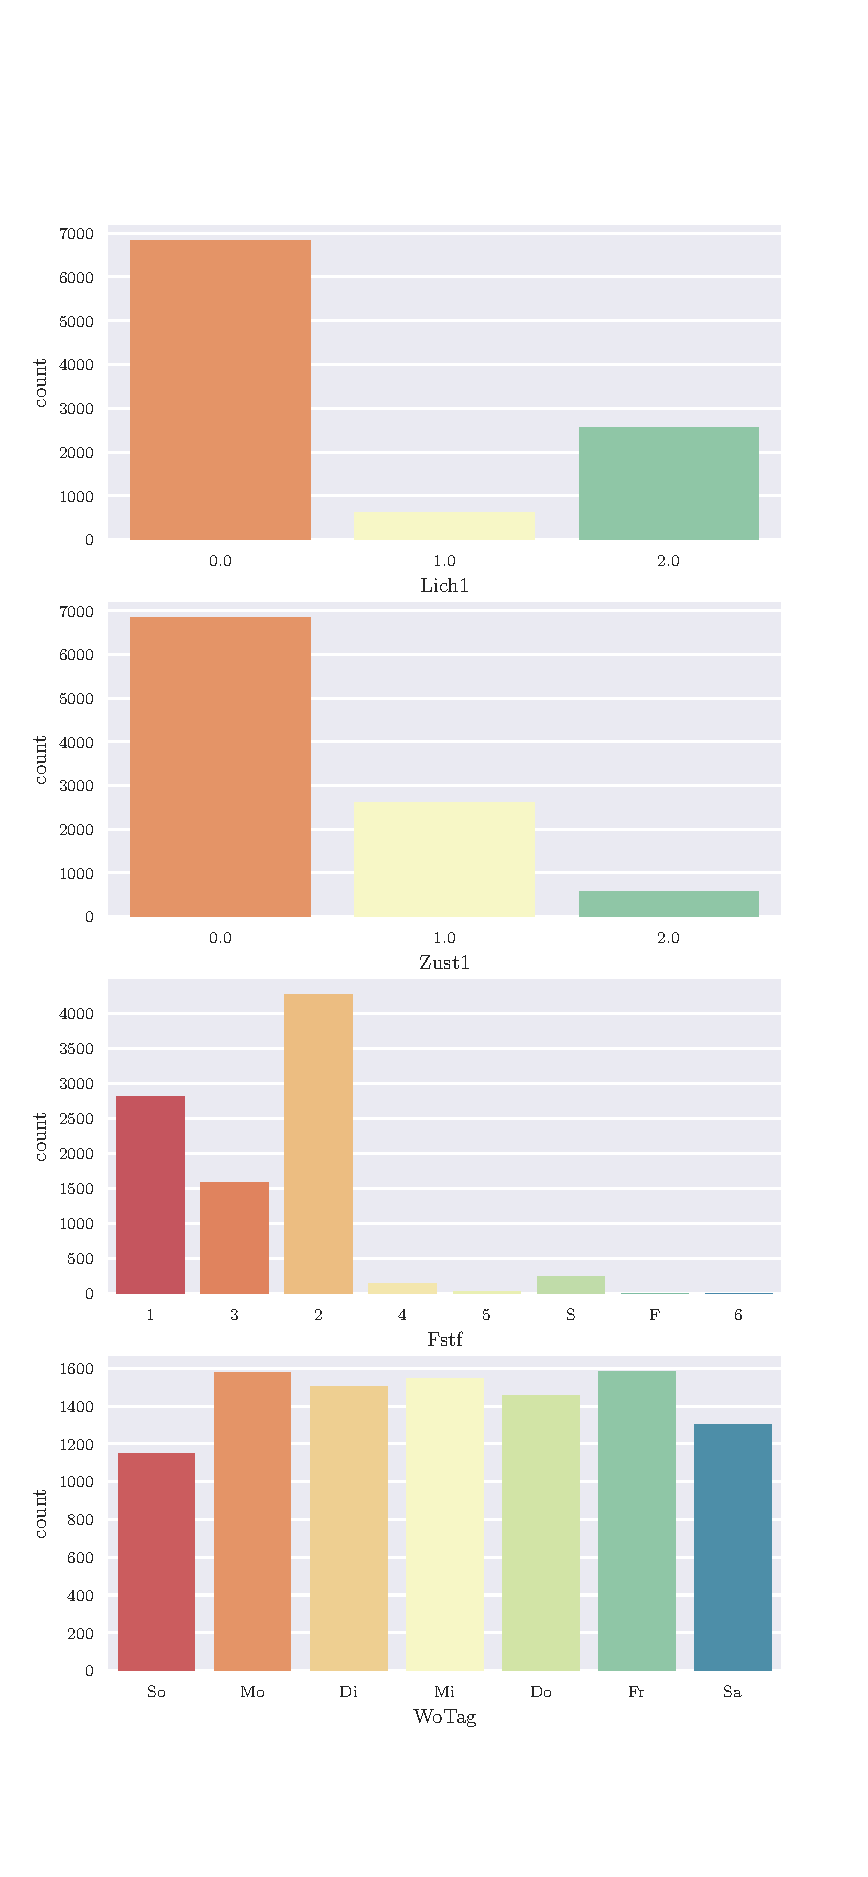
\includegraphics[scale=0.7]{CorrAnalysis/data/BAYSIS/01_dataset/plots/baysis_dataset_count_multiple03}
        \caption{Distribution of the accident category Lich, Zust, Fstf and WoTag}
        \label{img:baysis_dataset_Lich}
        \label{img:baysis_dataset_Zust}
        \label{img:baysis_dataset_Fstf}
        \label{img:baysis_dataset_WoTag}
    \end{figure}

    % ------- BAYSIS Dataset - Tables --------
    % \newgeometry{left=1cm,right=1cm,top=1cm}
    \begin{sidewaystable}
        \tiny
        \setlength{\tabcolsep}{4pt}
        \centering
        \begin{tabular}{lrrrrrrrrrrrrrrrrrrrr}
\toprule
{} &  Strasse &  Kat &  Typ &  Betei &  UArt1 &  UArt2 &  AUrs1 &  AUrs2 &  AufHi &  Alkoh &  Char1 &  Char2 &  Lich1 &  Lich2 &  Zust1 &  Zust2 &  Fstf &  WoTag &  FeiTag &  Month \\
\midrule
Strasse &     1.00 & 0.07 & 0.11 &   0.08 &   0.09 &   0.05 &   0.07 &   0.04 &   0.08 &   0.07 &   0.12 &   0.10 &   0.05 &   0.06 &   0.10 &   0.06 &  0.15 &   0.09 &    0.05 &   0.05 \\
Kat     &     0.07 & 1.00 & 0.16 &   0.18 &   0.31 &   0.10 &   0.08 &   0.05 &   0.12 &   0.02 &   0.05 &   0.03 &   0.02 &   0.04 &   0.05 &   0.02 &  0.08 &   0.04 &    0.03 &   0.05 \\
Typ     &     0.11 & 0.16 & 1.00 &   0.31 &   0.56 &   0.06 &   0.26 &   0.06 &   0.25 &   0.06 &   0.15 &   0.09 &   0.09 &   0.20 &   0.33 &   0.12 &  0.16 &   0.08 &    0.05 &   0.09 \\
Betei   &     0.08 & 0.18 & 0.31 &   1.00 &   0.28 &   0.06 &   0.14 &   0.20 &   0.24 &   0.04 &   0.07 &   0.07 &   0.09 &   0.09 &   0.25 &   0.10 &  0.08 &   0.07 &    0.06 &   0.06 \\
UArt1   &     0.09 & 0.31 & 0.56 &   0.28 &   1.00 &   0.08 &   0.21 &   0.05 &   0.32 &   0.05 &   0.14 &   0.09 &   0.10 &   0.22 &   0.25 &   0.09 &  0.16 &   0.08 &    0.05 &   0.06 \\
UArt2   &     0.05 & 0.10 & 0.06 &   0.06 &   0.08 &   1.00 &   0.06 &   0.03 &   0.15 &   0.04 &   0.03 &   0.05 &   0.03 &   0.05 &   0.08 &   0.04 &  0.04 &   0.04 &    0.01 &   0.04 \\
AUrs1   &     0.07 & 0.08 & 0.26 &   0.14 &   0.21 &   0.06 &   1.00 &   0.20 &   0.16 &   0.05 &   0.08 &   0.09 &   0.12 &   0.13 &   0.66 &   0.77 &  0.05 &   0.09 &    0.04 &   0.15 \\
AUrs2   &     0.04 & 0.05 & 0.06 &   0.20 &   0.05 &   0.03 &   0.20 &   1.00 &   0.06 &   0.04 &   0.03 &   0.06 &   0.04 &   0.03 &   0.12 &   0.33 &  0.03 &   0.03 &    0.03 &   0.05 \\
AufHi   &     0.08 & 0.12 & 0.25 &   0.24 &   0.32 &   0.15 &   0.16 &   0.06 &   1.00 &   0.04 &   0.08 &   0.10 &   0.08 &   0.10 &   0.25 &   0.09 &  0.06 &   0.07 &    0.04 &   0.06 \\
Alkoh   &     0.07 & 0.02 & 0.06 &   0.04 &   0.05 &   0.04 &   0.05 &   0.04 &   0.04 &   1.00 &   0.02 &   0.00 &   0.11 &   0.11 &   0.03 &   0.01 &  0.05 &   0.08 &    0.01 &   0.05 \\
Char1   &     0.12 & 0.05 & 0.15 &   0.07 &   0.14 &   0.03 &   0.08 &   0.03 &   0.08 &   0.02 &   1.00 &   0.58 &   0.04 &   0.05 &   0.10 &   0.03 &  0.06 &   0.03 &    0.02 &   0.04 \\
Char2   &     0.10 & 0.03 & 0.09 &   0.07 &   0.09 &   0.05 &   0.09 &   0.06 &   0.10 &   0.00 &   0.58 &   1.00 &   0.04 &   0.04 &   0.08 &   0.03 &  0.08 &   0.03 &    0.02 &   0.04 \\
Lich1   &     0.05 & 0.02 & 0.09 &   0.09 &   0.10 &   0.03 &   0.12 &   0.04 &   0.08 &   0.11 &   0.04 &   0.04 &   1.00 &   0.71 &   0.16 &   0.06 &  0.05 &   0.04 &    0.03 &   0.21 \\
Lich2   &     0.06 & 0.04 & 0.20 &   0.09 &   0.22 &   0.05 &   0.13 &   0.03 &   0.10 &   0.11 &   0.05 &   0.04 &   0.71 &   1.00 &   0.16 &   0.06 &  0.17 &   0.04 &    0.03 &   0.20 \\
Zust1   &     0.10 & 0.05 & 0.33 &   0.25 &   0.25 &   0.08 &   0.66 &   0.12 &   0.25 &   0.03 &   0.10 &   0.08 &   0.16 &   0.16 &   1.00 &   0.17 &  0.06 &   0.12 &    0.05 &   0.37 \\
Zust2   &     0.06 & 0.02 & 0.12 &   0.10 &   0.09 &   0.04 &   0.77 &   0.33 &   0.09 &   0.01 &   0.03 &   0.03 &   0.06 &   0.06 &   0.17 &   1.00 &  0.05 &   0.06 &    0.02 &   0.17 \\
Fstf    &     0.15 & 0.08 & 0.16 &   0.08 &   0.16 &   0.04 &   0.05 &   0.03 &   0.06 &   0.05 &   0.06 &   0.08 &   0.05 &   0.17 &   0.06 &   0.05 &  1.00 &   0.03 &    0.02 &   0.04 \\
WoTag   &     0.09 & 0.04 & 0.08 &   0.07 &   0.08 &   0.04 &   0.09 &   0.03 &   0.07 &   0.08 &   0.03 &   0.03 &   0.04 &   0.04 &   0.12 &   0.06 &  0.03 &   1.00 &    0.13 &   0.09 \\
FeiTag  &     0.05 & 0.03 & 0.05 &   0.06 &   0.05 &   0.01 &   0.04 &   0.03 &   0.04 &   0.01 &   0.02 &   0.02 &   0.03 &   0.03 &   0.05 &   0.02 &  0.02 &   0.13 &    1.00 &   0.13 \\
Month   &     0.05 & 0.05 & 0.09 &   0.06 &   0.06 &   0.04 &   0.15 &   0.05 &   0.06 &   0.05 &   0.04 &   0.04 &   0.21 &   0.20 &   0.37 &   0.17 &  0.04 &   0.09 &    0.13 &   1.00 \\
\bottomrule
\end{tabular}

        \caption{Correlation matrix for BAYSIS dataset, calculated with Cramer's $V$, $\eta$, $\tau$, $r_{pq}$, $r$}
        \label{table:appendix_correlation_matrix_dataset_cramers}
    \end{sidewaystable}
    \begin{sidewaystable}
        \tiny
        \setlength{\tabcolsep}{4pt}
        \centering
        \begin{tabular}{lrrrrrrrrrrrrrrrrrrrr}
\toprule
{} &  Strasse &  Kat &  Typ &  Betei &  UArt1 &  UArt2 &  AUrs1 &  AUrs2 &  AufHi &  Alkoh &  Char1 &  Char2 &  Lich1 &  Lich2 &  Zust1 &  Zust2 &  Fstf &  WoTag &  FeiTag &  Month \\
\midrule
Strasse &     1.00 & 0.00 & 0.02 &   0.01 &   0.01 &   0.00 &   0.01 &   0.00 &   0.01 &   0.00 &   0.01 &   0.00 &   0.00 &   0.00 &   0.00 &   0.00 &  0.04 &   0.01 &    0.00 &   0.01 \\
Kat     &     0.01 & 1.00 & 0.04 &   0.05 &   0.16 &   0.02 &   0.01 &   0.00 &   0.01 &   0.00 &   0.00 &   0.00 &   0.00 &   0.00 &   0.00 &   0.00 &  0.01 &   0.00 &    0.00 &   0.00 \\
Typ     &     0.03 & 0.03 & 1.00 &   0.26 &   0.39 &   0.01 &   0.15 &   0.01 &   0.17 &   0.00 &   0.02 &   0.00 &   0.01 &   0.02 &   0.09 &   0.01 &  0.05 &   0.02 &    0.00 &   0.02 \\
Betei   &     0.02 & 0.04 & 0.29 &   1.00 &   0.36 &   0.01 &   0.09 &   0.01 &   0.22 &   0.00 &   0.01 &   0.00 &   0.01 &   0.01 &   0.05 &   0.01 &  0.02 &   0.02 &    0.00 &   0.01 \\
UArt1   &     0.02 & 0.07 & 0.25 &   0.20 &   1.00 &   0.02 &   0.07 &   0.00 &   0.25 &   0.00 &   0.01 &   0.00 &   0.01 &   0.01 &   0.03 &   0.00 &  0.05 &   0.01 &    0.00 &   0.01 \\
UArt2   &     0.02 & 0.03 & 0.02 &   0.03 &   0.07 &   1.00 &   0.02 &   0.00 &   0.20 &   0.00 &   0.01 &   0.00 &   0.00 &   0.01 &   0.01 &   0.00 &  0.01 &   0.01 &    0.00 &   0.01 \\
AUrs1   &     0.05 & 0.01 & 0.25 &   0.14 &   0.18 &   0.01 &   1.00 &   0.04 &   0.14 &   0.00 &   0.02 &   0.01 &   0.02 &   0.02 &   0.38 &   0.05 &  0.01 &   0.03 &    0.00 &   0.14 \\
AUrs2   &     0.09 & 0.02 & 0.12 &   0.10 &   0.12 &   0.02 &   0.37 &   1.00 &   0.08 &   0.01 &   0.02 &   0.01 &   0.02 &   0.01 &   0.16 &   0.25 &  0.05 &   0.05 &    0.01 &   0.13 \\
AufHi   &     0.03 & 0.01 & 0.22 &   0.25 &   0.50 &   0.11 &   0.11 &   0.01 &   1.00 &   0.00 &   0.02 &   0.01 &   0.01 &   0.01 &   0.07 &   0.01 &  0.02 &   0.02 &    0.00 &   0.02 \\
Alkoh   &     0.01 & 0.00 & 0.01 &   0.01 &   0.02 &   0.01 &   0.02 &   0.00 &   0.01 &   1.00 &   0.00 &   0.00 &   0.05 &   0.05 &   0.00 &   0.00 &  0.01 &   0.03 &    0.00 &   0.01 \\
Char1   &     0.06 & 0.01 & 0.05 &   0.03 &   0.05 &   0.01 &   0.03 &   0.00 &   0.03 &   0.00 &   1.00 &   0.14 &   0.00 &   0.00 &   0.02 &   0.00 &  0.02 &   0.01 &    0.00 &   0.01 \\
Char2   &     0.05 & 0.00 & 0.03 &   0.02 &   0.03 &   0.01 &   0.03 &   0.01 &   0.04 &   0.00 &   0.60 &   1.00 &   0.01 &   0.01 &   0.03 &   0.00 &  0.02 &   0.00 &    0.00 &   0.01 \\
Lich1   &     0.00 & 0.00 & 0.01 &   0.01 &   0.01 &   0.00 &   0.02 &   0.00 &   0.01 &   0.01 &   0.00 &   0.00 &   1.00 &   0.80 &   0.03 &   0.00 &  0.00 &   0.00 &    0.00 &   0.06 \\
Lich2   &     0.01 & 0.00 & 0.03 &   0.01 &   0.04 &   0.00 &   0.02 &   0.00 &   0.02 &   0.01 &   0.00 &   0.00 &   0.90 &   1.00 &   0.04 &   0.00 &  0.03 &   0.00 &    0.00 &   0.06 \\
Zust1   &     0.01 & 0.00 & 0.14 &   0.08 &   0.08 &   0.01 &   0.36 &   0.02 &   0.08 &   0.00 &   0.01 &   0.00 &   0.03 &   0.03 &   1.00 &   0.04 &  0.00 &   0.02 &    0.00 &   0.14 \\
Zust2   &     0.03 & 0.01 & 0.13 &   0.08 &   0.07 &   0.01 &   0.38 &   0.19 &   0.08 &   0.00 &   0.01 &   0.00 &   0.03 &   0.03 &   0.28 &   1.00 &  0.02 &   0.02 &    0.00 &   0.24 \\
Fstf    &     0.06 & 0.01 & 0.04 &   0.02 &   0.06 &   0.00 &   0.01 &   0.00 &   0.01 &   0.00 &   0.01 &   0.00 &   0.00 &   0.01 &   0.00 &   0.00 &  1.00 &   0.00 &    0.00 &   0.00 \\
WoTag   &     0.01 & 0.00 & 0.01 &   0.01 &   0.01 &   0.00 &   0.01 &   0.00 &   0.01 &   0.00 &   0.00 &   0.00 &   0.00 &   0.00 &   0.01 &   0.00 &  0.00 &   1.00 &    0.00 &   0.01 \\
FeiTag  &     0.01 & 0.00 & 0.01 &   0.01 &   0.01 &   0.00 &   0.01 &   0.00 &   0.01 &   0.00 &   0.00 &   0.00 &   0.00 &   0.00 &   0.01 &   0.00 &  0.00 &   0.07 &    1.00 &   0.10 \\
Month   &     0.01 & 0.00 & 0.01 &   0.01 &   0.01 &   0.00 &   0.04 &   0.00 &   0.01 &   0.00 &   0.00 &   0.00 &   0.02 &   0.02 &   0.04 &   0.01 &  0.00 &   0.01 &    0.00 &   1.00 \\
\bottomrule
\end{tabular}

        \caption{Correlation matrix for BAYSIS dataset, calculated with Theil's $U$, $\eta$, $\tau$, $r_{pq}$, $r$}
        \label{table:appendix_correlation_matrix_dataset_theils}
    \end{sidewaystable}
    \begin{sidewaystable}
        \tiny
        \setlength{\tabcolsep}{4pt}
        \centering
        \begin{tabular}{lrrrrrrrrrrrrrrrrrrrr}
\toprule
{} &  Strasse &   Kat &   Typ &  Betei &  UArt1 &  UArt2 &  AUrs1 &  AUrs2 &  AufHi &  Alkoh &  Char1 &  Char2 &  Lich1 &  Lich2 &  Zust1 &  Zust2 &  Fstf &  WoTag &  FeiTag &  Month \\
\midrule
Strasse &      nan & 0.000 & 0.000 &  0.000 &  0.000 &  0.000 &  0.000 &  0.871 &  0.000 &  0.000 &  0.000 &  0.000 &  0.165 &  0.000 &  0.000 &  0.006 & 0.000 &  0.000 &   0.073 &  0.002 \\
Kat     &    0.000 &   nan & 0.000 &  0.000 &  0.000 &  0.000 &  0.000 &  0.000 &  0.000 &  0.225 &  0.000 &  0.058 &  0.260 &  0.000 &  0.000 &  0.068 & 0.000 &  0.000 &   0.069 &  0.000 \\
Typ     &    0.000 & 0.000 &   nan &  0.000 &  0.000 &  0.000 &  0.000 &  0.000 &  0.000 &  0.000 &  0.000 &  0.000 &  0.000 &  0.000 &  0.000 &  0.000 & 0.000 &  0.000 &   0.000 &  0.000 \\
Betei   &    0.000 & 0.000 & 0.000 &    nan &  0.000 &  0.000 &  0.000 &  0.000 &  0.000 &  0.463 &  0.000 &  0.000 &  0.000 &  0.000 &  0.000 &  0.000 & 0.000 &  0.000 &   0.000 &  0.000 \\
UArt1   &    0.000 & 0.000 & 0.000 &  0.000 &    nan &  0.000 &  0.000 &  0.000 &  0.000 &  0.000 &  0.000 &  0.000 &  0.000 &  0.000 &  0.000 &  0.000 & 0.000 &  0.000 &   0.001 &  0.000 \\
UArt2   &    0.000 & 0.000 & 0.000 &  0.000 &  0.000 &    nan &  0.000 &  0.045 &  0.000 &  0.017 &  0.043 &  0.001 &  0.122 &  0.001 &  0.000 &  0.002 & 0.000 &  0.016 &   0.998 &  0.054 \\
AUrs1   &    0.000 & 0.000 & 0.000 &  0.000 &  0.000 &  0.000 &    nan &  0.000 &  0.000 &  0.157 &  0.000 &  0.000 &  0.000 &  0.000 &  0.000 &  0.000 & 0.002 &  0.000 &   0.386 &  0.000 \\
AUrs2   &    0.871 & 0.000 & 0.000 &  0.000 &  0.000 &  0.045 &  0.000 &    nan &  0.000 &  0.070 &  0.130 &  0.000 &  0.028 &  0.647 &  0.000 &  0.000 & 0.247 &  0.100 &   0.199 &  0.000 \\
AufHi   &    0.000 & 0.000 & 0.000 &  0.000 &  0.000 &  0.000 &  0.000 &  0.000 &    nan &  0.026 &  0.000 &  0.000 &  0.000 &  0.000 &  0.000 &  0.000 & 0.000 &  0.000 &   0.066 &  0.000 \\
Alkoh   &    0.000 & 0.225 & 0.000 &  0.463 &  0.000 &  0.017 &  0.157 &  0.070 &  0.026 &    nan &  0.689 &  0.754 &  0.000 &  0.000 &  0.035 &  0.745 & 0.004 &  0.000 &   0.279 &  0.017 \\
Char1   &    0.000 & 0.000 & 0.000 &  0.000 &  0.000 &  0.043 &  0.000 &  0.130 &  0.000 &  0.689 &    nan &  0.000 &  0.000 &  0.000 &  0.000 &  0.017 & 0.000 &  0.007 &   0.415 &  0.084 \\
Char2   &    0.000 & 0.058 & 0.000 &  0.000 &  0.000 &  0.001 &  0.000 &  0.000 &  0.000 &  0.754 &  0.000 &    nan &  0.001 &  0.000 &  0.000 &  0.012 & 0.000 &  0.250 &   0.020 &  0.075 \\
Lich1   &    0.165 & 0.260 & 0.000 &  0.000 &  0.000 &  0.122 &  0.000 &  0.028 &  0.000 &  0.000 &  0.000 &  0.001 &    nan &  0.000 &  0.000 &  0.000 & 0.000 &  0.002 &   0.015 &  0.000 \\
Lich2   &    0.000 & 0.000 & 0.000 &  0.000 &  0.000 &  0.001 &  0.000 &  0.647 &  0.000 &  0.000 &  0.000 &  0.000 &  0.000 &    nan &  0.000 &  0.000 & 0.000 &  0.001 &   0.033 &  0.000 \\
Zust1   &    0.000 & 0.000 & 0.000 &  0.000 &  0.000 &  0.000 &  0.000 &  0.000 &  0.000 &  0.035 &  0.000 &  0.000 &  0.000 &  0.000 &    nan &  0.000 & 0.000 &  0.000 &   0.000 &  0.000 \\
Zust2   &    0.006 & 0.068 & 0.000 &  0.000 &  0.000 &  0.002 &  0.000 &  0.000 &  0.000 &  0.745 &  0.017 &  0.012 &  0.000 &  0.000 &  0.000 &    nan & 0.000 &  0.000 &   0.125 &  0.000 \\
Fstf    &    0.000 & 0.000 & 0.000 &  0.000 &  0.000 &  0.000 &  0.002 &  0.247 &  0.000 &  0.004 &  0.000 &  0.000 &  0.000 &  0.000 &  0.000 &  0.000 &   nan &  0.033 &   0.660 &  0.081 \\
WoTag   &    0.000 & 0.000 & 0.000 &  0.000 &  0.000 &  0.016 &  0.000 &  0.100 &  0.000 &  0.000 &  0.007 &  0.250 &  0.002 &  0.001 &  0.000 &  0.000 & 0.033 &    nan &   0.000 &  0.000 \\
FeiTag  &    0.073 & 0.069 & 0.000 &  0.000 &  0.001 &  0.998 &  0.386 &  0.199 &  0.066 &  0.279 &  0.415 &  0.020 &  0.015 &  0.033 &  0.000 &  0.125 & 0.660 &  0.000 &     nan &  0.000 \\
Month   &    0.002 & 0.000 & 0.000 &  0.000 &  0.000 &  0.054 &  0.000 &  0.000 &  0.000 &  0.017 &  0.084 &  0.075 &  0.000 &  0.000 &  0.000 &  0.000 & 0.081 &  0.000 &   0.000 &    nan \\
\bottomrule
\end{tabular}

        \caption{Significancy matrix for BAYSIS dataset}
        \label{table:appendix_significancy_matrix_dataset}
    \end{sidewaystable}
    \begin{sidewaystable}
        \tiny
        \setlength{\tabcolsep}{4pt}
        \centering
        \begin{tabular}{lllllllllllllllllllll}
\toprule
{} & Strasse &  Kat &  Typ & Betei & UArt1 & UArt2 & AUrs1 & AUrs2 & AufHi & Alkoh & Char1 & Char2 & Lich1 & Lich2 & Zust1 & Zust2 & Fstf & WoTag & FeiTag & Month \\
\midrule
Strasse &     NaN &  $V$ &  $V$ &   $V$ &   $V$ &   $V$ &   $V$ &   $V$ &   $V$ &   $V$ &   $V$ &   $V$ &   $V$ &   $V$ &   $V$ &   $V$ &  $V$ &   $V$ &    $V$ &   $V$ \\
Kat     &     $V$ &  NaN &  $V$ &   $V$ &   $V$ &   $V$ &   $V$ &   $V$ &   $V$ &   $V$ &   $V$ &   $V$ &   $V$ &   $V$ &   $V$ &   $V$ &  $V$ &   $V$ &    $V$ &   $V$ \\
Typ     &     $V$ &  $V$ &  NaN &   $V$ &   $V$ &   $V$ &   $V$ &   $V$ &   $V$ &   $V$ &   $V$ &   $V$ &   $V$ &   $V$ &   $V$ &   $V$ &  $V$ &   $V$ &    $V$ &   $V$ \\
Betei   &     $V$ &  $V$ &  $V$ &   NaN &   $V$ &   $V$ &   $V$ &   $V$ &   $V$ &   $V$ &   $V$ &   $V$ &   $V$ &   $V$ &   $V$ &   $V$ &  $V$ &   $V$ &    $V$ &   $V$ \\
UArt1   &     $V$ &  $V$ &  $V$ &   $V$ &   NaN &   $V$ &   $V$ &   $V$ &   $V$ &   $V$ &   $V$ &   $V$ &   $V$ &   $V$ &   $V$ &   $V$ &  $V$ &   $V$ &    $V$ &   $V$ \\
UArt2   &     $V$ &  $V$ &  $V$ &   $V$ &   $V$ &   NaN &   $V$ &   $V$ &   $V$ &   $V$ &   $V$ &   $V$ &   $V$ &   $V$ &   $V$ &   $V$ &  $V$ &   $V$ &    $V$ &   $V$ \\
AUrs1   &     $V$ &  $V$ &  $V$ &   $V$ &   $V$ &   $V$ &   NaN &   $V$ &   $V$ &   $V$ &   $V$ &   $V$ &   $V$ &   $V$ &   $V$ &   $V$ &  $V$ &   $V$ &    $V$ &   $V$ \\
AUrs2   &     $V$ &  $V$ &  $V$ &   $V$ &   $V$ &   $V$ &   $V$ &   NaN &   $V$ &   $V$ &   $V$ &   $V$ &   $V$ &   $V$ &   $V$ &   $V$ &  $V$ &   $V$ &    $V$ &   $V$ \\
AufHi   &     $V$ &  $V$ &  $V$ &   $V$ &   $V$ &   $V$ &   $V$ &   $V$ &   NaN &   $V$ &   $V$ &   $V$ &   $V$ &   $V$ &   $V$ &   $V$ &  $V$ &   $V$ &    $V$ &   $V$ \\
Alkoh   &     $V$ &  $V$ &  $V$ &   $V$ &   $V$ &   $V$ &   $V$ &   $V$ &   $V$ &   NaN &   $V$ &   $V$ &   $V$ &   $V$ &   $V$ &   $V$ &  $V$ &   $V$ &    $V$ &   $V$ \\
Char1   &     $V$ &  $V$ &  $V$ &   $V$ &   $V$ &   $V$ &   $V$ &   $V$ &   $V$ &   $V$ &   NaN &   $V$ &   $V$ &   $V$ &   $V$ &   $V$ &  $V$ &   $V$ &    $V$ &   $V$ \\
Char2   &     $V$ &  $V$ &  $V$ &   $V$ &   $V$ &   $V$ &   $V$ &   $V$ &   $V$ &   $V$ &   $V$ &   NaN &   $V$ &   $V$ &   $V$ &   $V$ &  $V$ &   $V$ &    $V$ &   $V$ \\
Lich1   &     $V$ &  $V$ &  $V$ &   $V$ &   $V$ &   $V$ &   $V$ &   $V$ &   $V$ &   $V$ &   $V$ &   $V$ &   NaN &   $V$ &   $V$ &   $V$ &  $V$ &   $V$ &    $V$ &   $V$ \\
Lich2   &     $V$ &  $V$ &  $V$ &   $V$ &   $V$ &   $V$ &   $V$ &   $V$ &   $V$ &   $V$ &   $V$ &   $V$ &   $V$ &   NaN &   $V$ &   $V$ &  $V$ &   $V$ &    $V$ &   $V$ \\
Zust1   &     $V$ &  $V$ &  $V$ &   $V$ &   $V$ &   $V$ &   $V$ &   $V$ &   $V$ &   $V$ &   $V$ &   $V$ &   $V$ &   $V$ &   NaN &   $V$ &  $V$ &   $V$ &    $V$ &   $V$ \\
Zust2   &     $V$ &  $V$ &  $V$ &   $V$ &   $V$ &   $V$ &   $V$ &   $V$ &   $V$ &   $V$ &   $V$ &   $V$ &   $V$ &   $V$ &   $V$ &   NaN &  $V$ &   $V$ &    $V$ &   $V$ \\
Fstf    &     $V$ &  $V$ &  $V$ &   $V$ &   $V$ &   $V$ &   $V$ &   $V$ &   $V$ &   $V$ &   $V$ &   $V$ &   $V$ &   $V$ &   $V$ &   $V$ &  NaN &   $V$ &    $V$ &   $V$ \\
WoTag   &     $V$ &  $V$ &  $V$ &   $V$ &   $V$ &   $V$ &   $V$ &   $V$ &   $V$ &   $V$ &   $V$ &   $V$ &   $V$ &   $V$ &   $V$ &   $V$ &  $V$ &   NaN &    $V$ &   $V$ \\
FeiTag  &     $V$ &  $V$ &  $V$ &   $V$ &   $V$ &   $V$ &   $V$ &   $V$ &   $V$ &   $V$ &   $V$ &   $V$ &   $V$ &   $V$ &   $V$ &   $V$ &  $V$ &   $V$ &    NaN &   $V$ \\
Month   &     $V$ &  $V$ &  $V$ &   $V$ &   $V$ &   $V$ &   $V$ &   $V$ &   $V$ &   $V$ &   $V$ &   $V$ &   $V$ &   $V$ &   $V$ &   $V$ &  $V$ &   $V$ &    $V$ &   NaN \\
\bottomrule
\end{tabular}

        \caption{Coefficient matrix for BAYSIS dataset}
        \label{table:appendix_coefficient_matrix_dataset}
    \end{sidewaystable}
    % \restoregeometry
    
    % -------------------------------
    % ------- BAYSIS Matched --------
    % -------------------------------
    % \tocless\section{BAYSIS Matched Data}
    % \label{appendix_baysis_dataset}
    
    % ------- BAYSIS Matched - Figures --------
    \begin{figure}[ht!]
        \centering
        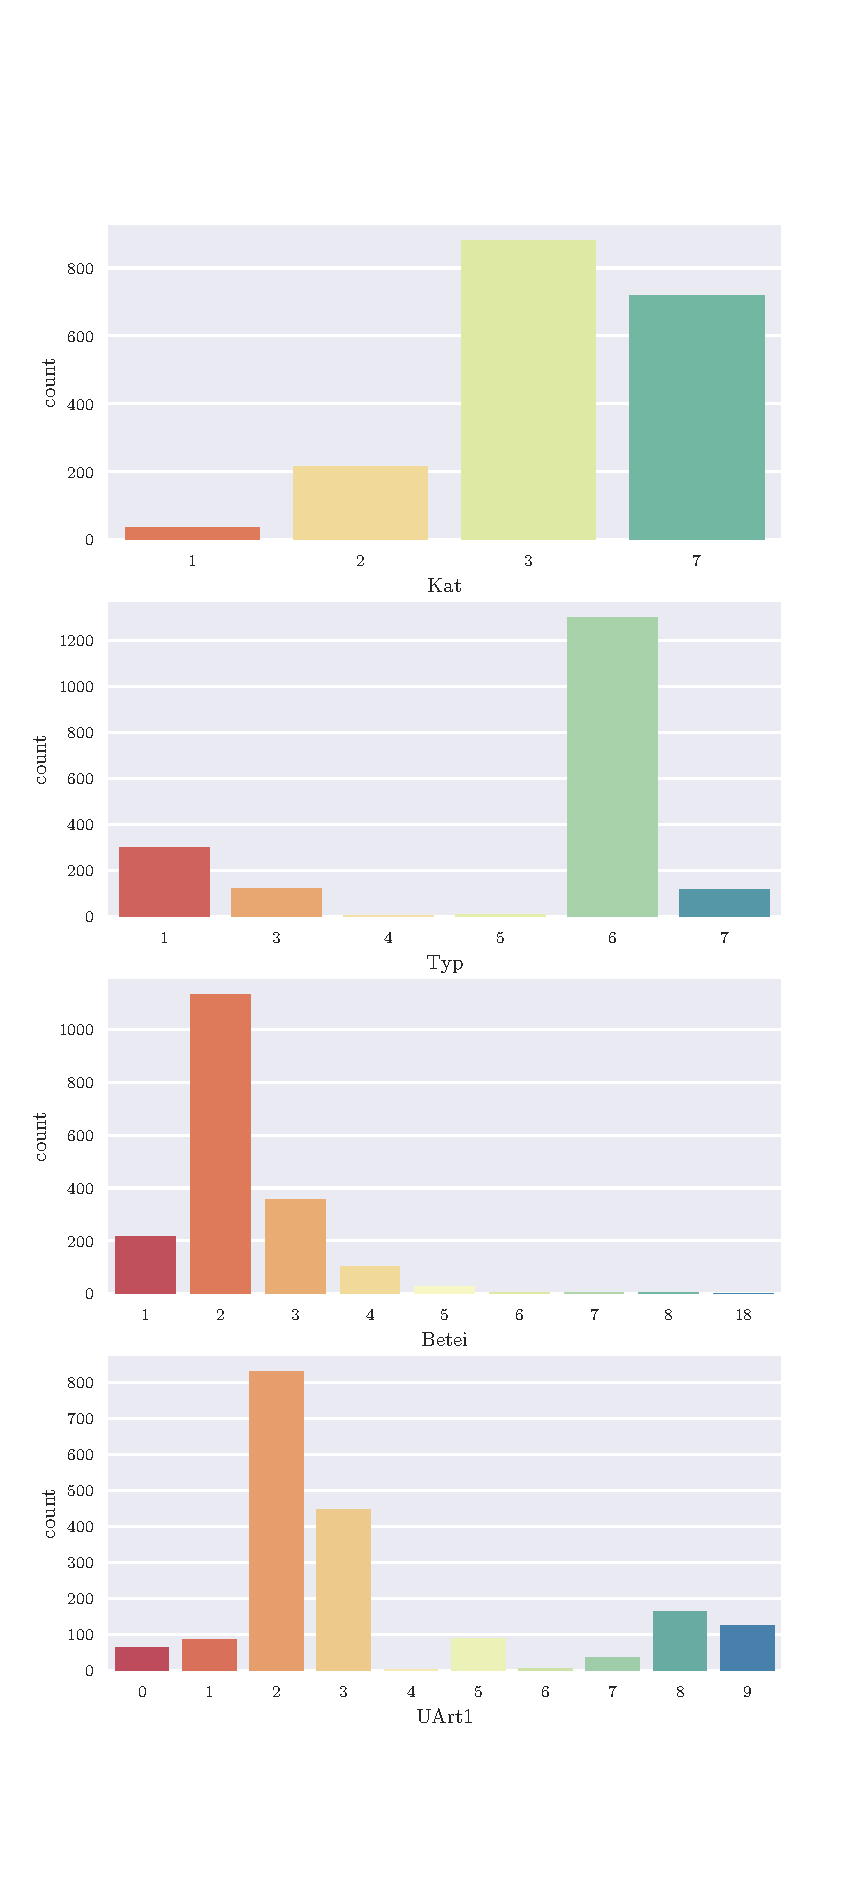
\includegraphics[scale=0.7]{CorrAnalysis/data/BAYSIS/02_matched/plots/baysis_matched_count_multiple01}
        \caption{Distribution of the accident category Kat, Typ, Betei and UArt}
        \label{img:baysis_matched_Kat}
        \label{img:baysis_matched_Typ}
        \label{img:baysis_matched_Betei}
        \label{img:baysis_matched_UArt}
    \end{figure}

    \begin{figure}[ht!]
        \centering
        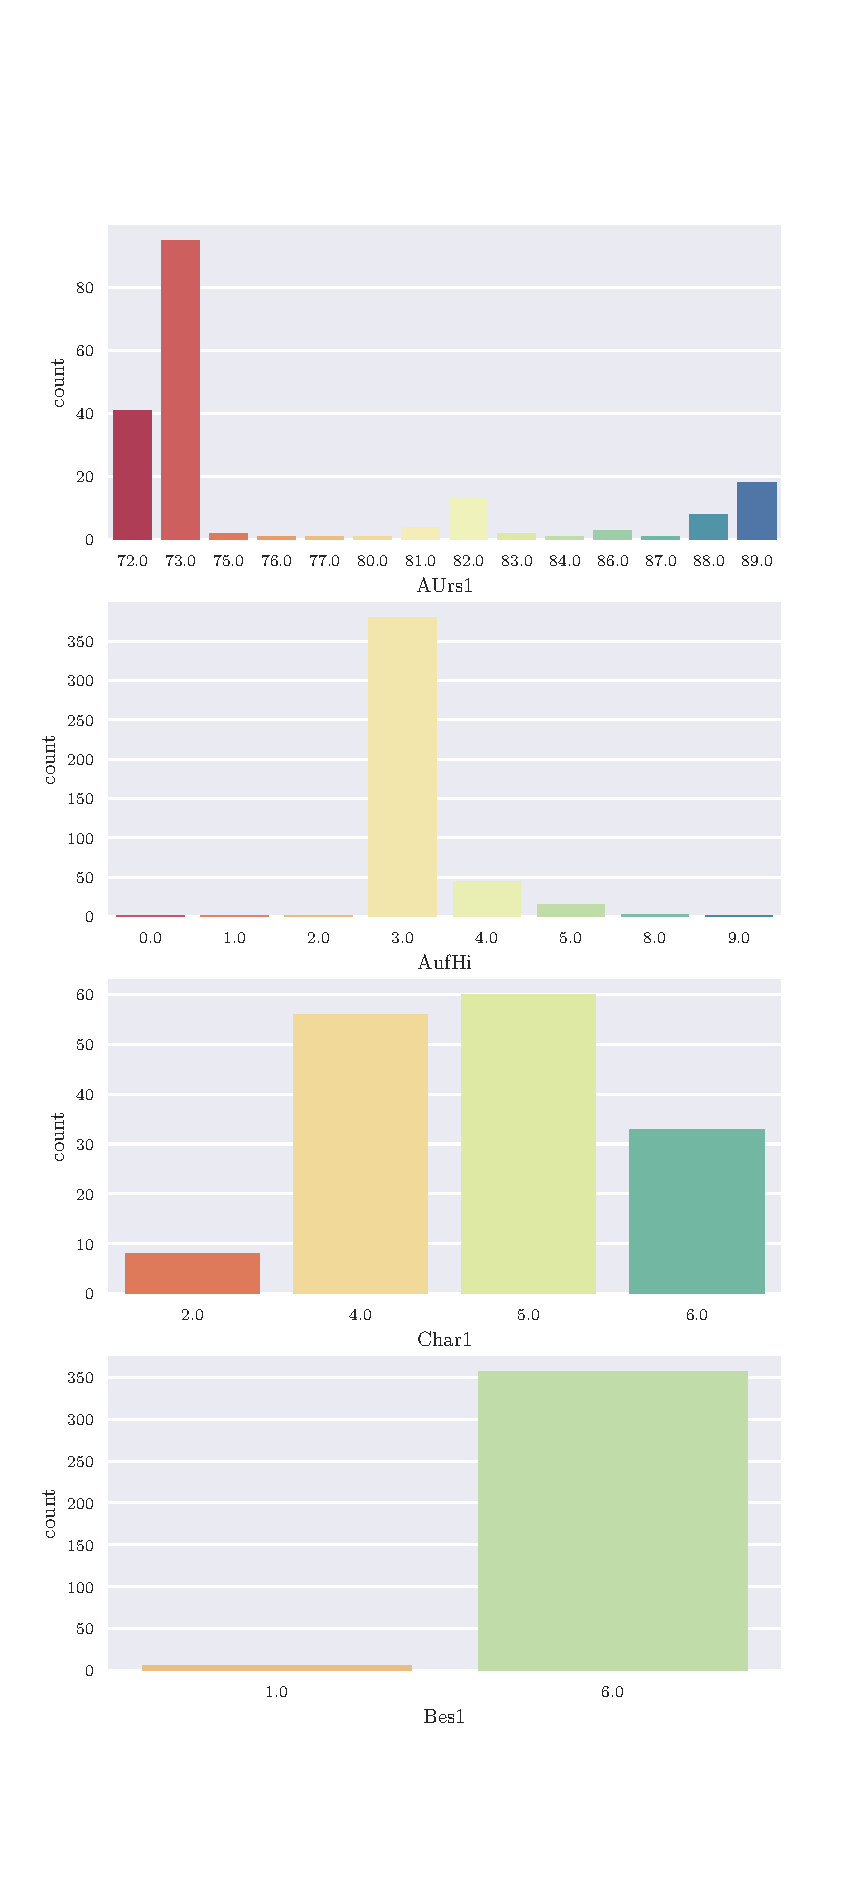
\includegraphics[scale=0.7]{CorrAnalysis/data/BAYSIS/02_matched/plots/baysis_matched_count_multiple02}
        \caption{Distribution of the accident category AUrs, AufHi, Char and Bes}
        \label{img:baysis_matched_AUrs}
        \label{img:baysis_matched_AufHi}
        \label{img:baysis_matched_Char}
        \label{img:baysis_matched_Bes}
    \end{figure}

    \begin{figure}[ht!]
        \centering
        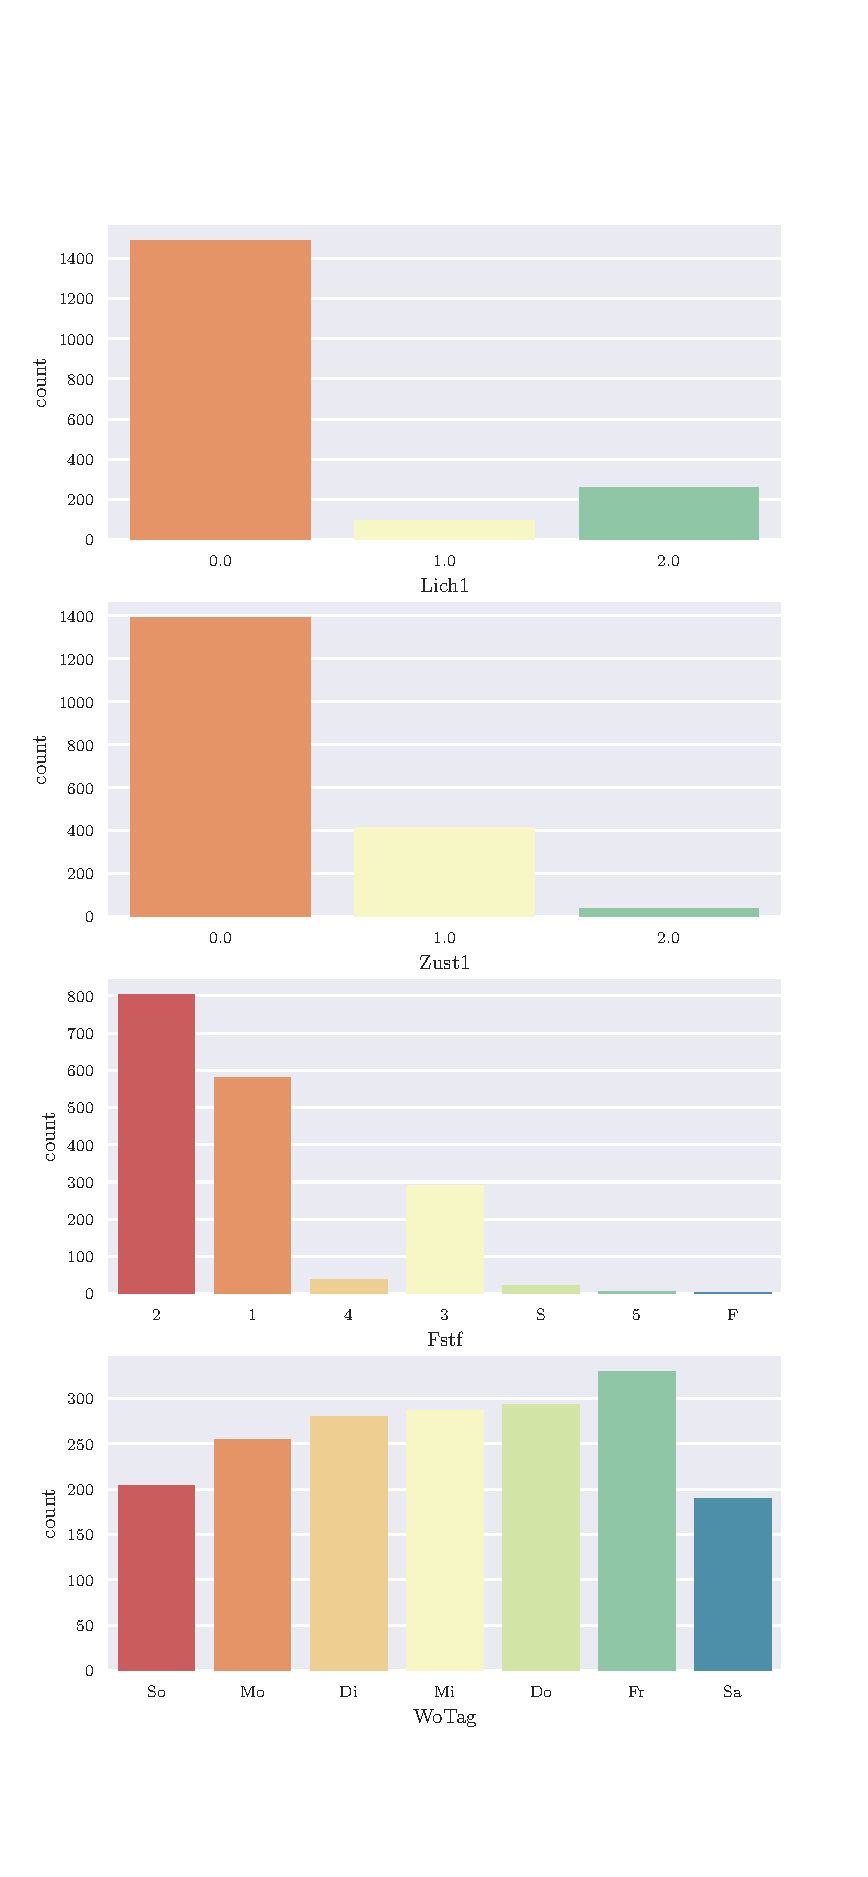
\includegraphics[scale=0.7]{CorrAnalysis/data/BAYSIS/02_matched/plots/baysis_matched_count_multiple03}
        \caption{Distribution of the accident category Lich, Zust, Fstf and WoTag}
        \label{img:baysis_matched_Lich}
        \label{img:baysis_matched_Zust}
        \label{img:baysis_matched_Fstf}
        \label{img:baysis_matched_WoTag}
    \end{figure}

    \begin{table}[ht!]
        \tiny
        \setlength{\tabcolsep}{4pt}
        \centering
        \begin{tabular}{rrrrrrrrrrrrrrrrr}
            \toprule
                    & A3 & A6 & A9 & A70 & A96 & A7 & A73 & A99 & A92 & A93 & A94 & A72 & A995 & A95 & A71 & A45 \\ 
            \midrule
            A6 		& 0.00 &  &  &  &  &  &  &  &  &  &  &  &  &  &  &  \\ 
            A9 		& \red{0.01} & 1.00 &  &  &  &  &  &  &  &  &  &  &  &  &  &  \\ 
            A70 	& \red{0.03} & 1.00 & 1.00 &  &  &  &  &  &  &  &  &  &  &  &  &  \\ 
            A96 	& \red{0.00} & 1.00 & 0.27 & 1.00 &  &  &  &  &  &  &  &  &  &  &  &  \\ 
            A7 		& \red{0.00} & 1.00 & 1.00 & 1.00 & 1.00 &  &  &  &  &  &  &  &  &  &  &  \\ 
            A73 	& \red{0.00} & 1.00 & 0.31 & 1.00 & 1.00 & 1.00 &  &  &  &  &  &  &  &  &  &  \\ 
            A99 	& 1.00 & 1.00 & 1.00 & 1.00 & 0.50 & 1.00 & 0.59 &  &  &  &  &  &  &  &  &  \\ 
            A92 	& \red{0.00} & 1.00 & 0.16 & 1.00 & 1.00 & 1.00 & 1.00 & 0.22 &  &  &  &  &  &  &  &  \\ 
            A93 	& 1.00 & 1.00 & 1.00 & 1.00 & 1.00 & 1.00 & 1.00 & 1.00 & 1.00 &  &  &  &  &  &  &  \\ 
            A94 	& \red{0.01} & 1.00 & 1.00 & 1.00 & 1.00 & 1.00 & 1.00 & 1.00 & 1.00 & 1.00 &  &  &  &  &  &  \\ 
            A72 	& 1.00 & 1.00 & 1.00 & 1.00 & 1.00 & 1.00 & 1.00 & 1.00 & 1.00 & 1.00 & 1.00 &  &  &  &  &  \\ 
            A995 	& 1.00 & 1.00 & 1.00 & 1.00 & 1.00 & 1.00 & 1.00 & 1.00 & 1.00 & 1.00 & 1.00 & 1.00 &  &  &  &  \\ 
            A95 	& 1.00 & 1.00 & 1.00 & 1.00 & 1.00 & 1.00 & 1.00 & 1.00 & 1.00 & 1.00 & 1.00 & 1.00 & 1.00 &  &  &  \\ 
            A71 	& 1.00 & 1.00 & 1.00 & 1.00 & 1.00 & 1.00 & 1.00 & 1.00 & 1.00 & 1.00 & 1.00 & 1.00 & 1.00 & 1.00 &  &  \\ 
            A45 	& 1.00 & 1.00 & 1.00 & 1.00 & 1.00 & 1.00 & 1.00 & 1.00 & 1.00 & 1.00 & 1.00 & 1.00 & 1.00 & 1.00 & 1.00 &  \\ 
            A980 	& 1.00 & 1.00 & 1.00 & 1.00 & 1.00 & 1.00 & 1.00 & 1.00 & 1.00 & 1.00 & 1.00 & 1.00 & 1.00 & 1.00 & 1.00 & 1.00 \\ 
            \bottomrule
        \end{tabular}
        \caption{Pairwise Wilcoxon $T$-test for \textit{Street} and \textit{Maximal Temporal Extent} complete}
        \label{tbl:wilcoxon_baysis_matched_Str_TMax_complete}
    \end{table}

    \begin{table}[ht!]
        \tiny
        \setlength{\tabcolsep}{4pt}
        \centering
        \begin{tabular}{rrrrrrrrrrrrrrrrr}
            \toprule
                    & A3 & A6 & A9 & A70 & A96 & A7 & A73 & A99 & A92 & A93 & A94 & A72 & A995 & A95 & A71 & A45 \\ 
            \midrule
            A6 	 & 0.84 &  &  &  &  &  &  &  &  &  &  &  &  &  &  &  \\ 
            A9 	 & 0.36 & 1.00 &  &  &  &  &  &  &  &  &  &  &  &  &  &  \\ 
            A70	 & 1.00 & 1.00 & 1.00 &  &  &  &  &  &  &  &  &  &  &  &  &  \\ 
            A96  & 0.10 & 1.00 & 1.00 & 1.00 &  &  &  &  &  &  &  &  &  &  &  &  \\ 
            A7 	 & 1.00 & 1.00 & 1.00 & 1.00 & 1.00 &  &  &  &  &  &  &  &  &  &  &  \\ 
            A73  & \red{0.00} & 1.00 & 0.51 & 1.00 & 1.00 & 1.00 &  &  &  &  &  &  &  &  &  &  \\ 
            A99  & \red{0.02} & 1.00 & 1.00 & 1.00 & 1.00 & 1.00 & 1.00 &  &  &  &  &  &  &  &  &  \\ 
            A92  & 0.26 & 1.00 & 1.00 & 1.00 & 1.00 & 1.00 & 1.00 & 1.00 &  &  &  &  &  &  &  &  \\ 
            A93  & 1.00 & 1.00 & 1.00 & 1.00 & 1.00 & 1.00 & 1.00 & 1.00 & 1.00 &  &  &  &  &  &  &  \\ 
            A94  & 0.28 & 1.00 & 1.00 & 1.00 & 1.00 & 1.00 & 1.00 & 1.00 & 1.00 & 1.00 &  &  &  &  &  &  \\ 
            A72  & 1.00 & 1.00 & 1.00 & 1.00 & 1.00 & 1.00 & 1.00 & 1.00 & 1.00 & 1.00 & 1.00 &  &  &  &  &  \\ 
            A995 & 1.00 & 1.00 & 1.00 & 1.00 & 1.00 & 1.00 & 1.00 & 1.00 & 1.00 & 1.00 & 1.00 & 1.00 &  &  &  &  \\ 
            A95  & 1.00 & 1.00 & 1.00 & 1.00 & 1.00 & 1.00 & 1.00 & 1.00 & 1.00 & 1.00 & 1.00 & 1.00 & 1.00 &  &  &  \\ 
            A71	 & 1.00 & 1.00 & 1.00 & 1.00 & 1.00 & 1.00 & 1.00 & 1.00 & 1.00 & 1.00 & 1.00 & 1.00 & 1.00 & 1.00 &  &  \\ 
            A45  & 1.00 & 1.00 & 1.00 & 1.00 & 1.00 & 1.00 & 1.00 & 1.00 & 1.00 & 1.00 & 1.00 & 1.00 & 1.00 & 1.00 & 1.00 &  \\ 
            A980 & 1.00 & 1.00 & 1.00 & 1.00 & 1.00 & 1.00 & 1.00 & 1.00 & 1.00 & 1.00 & 1.00 & 1.00 & 1.00 & 1.00 & 1.00 & 1.00 \\
            \bottomrule
        \end{tabular}
        \caption{Pairwise Wilcoxon $T$-test for \textit{Street} and \textit{Average Temporal Extent} complete}
        \label{tbl:wilcoxon_baysis_matched_Str_TAvg_complete}
    \end{table}

    \begin{table}[ht!]
        \tiny
        \setlength{\tabcolsep}{4pt}
        \centering
        \begin{tabular}{rrrrrrrrrrrrrrrrr}
            \toprule
                    & A3   & A6   & A9   & A70  & A96  & A7   & A73   & A99 & A92 & A93 & A94 & A72 & A995 & A95 & A71 & A45 \\ 
            \midrule
            A6 		& 0.40 &  &  &  &  &  &  &  &  &  &  &  &  &  &  &  \\ 
            A9 		& \red{0.00} & 1.00 &  &  &  &  &  &  &  &  &  &  &  &  &  &  \\ 
            A70 	& \red{0.00} & 0.83 & 0.54 &  &  &  &  &  &  &  &  &  &  &  &  &  \\ 
            A96 	& \red{0.00} & 1.00 & 0.14 & 1.00 &  &  &  &  &  &  &  &  &  &  &  &  \\ 
            A7 		& \red{0.00} & 1.00 & 1.00 & 1.00 & 1.00 &  &  &  &  &  &  &  &  &  &  &  \\ 
            A73 	& \red{0.00} & \red{0.00} & \red{0.00} & 1.00 & 1.00 & 0.59 &  &  &  &  &  &  &  &  &  &  \\ 
            A99 	& 1.00 & 1.00 & 1.00 & 0.80 & 0.31 & 1.00 & \red{0.00} &  &  &  &  &  &  &  &  &  \\ 
            A92 	& \red{0.00} & \red{0.00} & \red{0.00} & 1.00 & 1.00 & 1.00 & 1.00 & \red{0.00} &  &  &  &  &  &  &  &  \\ 
            A93 	& \red{0.03} & 1.00 & 1.00 & 1.00 & 1.00 & 1.00 & 1.00 & 1.00 & 1.00 &  &  &  &  &  &  &  \\ 
            A94 	& \red{0.00} & 0.11 & \red{0.03} & 1.00 & 1.00 & 1.00 & 1.00 & 0.09 & 1.00 & 1.00 &  &  &  &  &  &  \\ 
            A72 	& 1.00 & 1.00 & 1.00 & 1.00 & 1.00 & 1.00 & 1.00 & 1.00 & 1.00 & 1.00 & 1.00 &  &  &  &  &  \\ 
            A995 	& 1.00 & 1.00 & 1.00 & 1.00 & 1.00 & 1.00 & 1.00 & 1.00 & 1.00 & 1.00 & 1.00 & 1.00 &  &  &  &  \\ 
            A95 	& 1.00 & 1.00 & 1.00 & 1.00 & 1.00 & 1.00 & 1.00 & 1.00 & 1.00 & 1.00 & 1.00 & 1.00 & 1.00 &  &  &  \\ 
            A71 	& 1.00 & 1.00 & 1.00 & 1.00 & 1.00 & 1.00 & 1.00 & 1.00 & 1.00 & 1.00 & 1.00 & 1.00 & 1.00 & 1.00 &  &  \\ 
            A45 	& 1.00 & 1.00 & 1.00 & 1.00 & 1.00 & 1.00 & 1.00 & 1.00 & 1.00 & 1.00 & 1.00 & 1.00 & 1.00 & 1.00 & 1.00 &  \\ 
            A980 	& 1.00 & 1.00 & 1.00 & 1.00 & 1.00 & 1.00 & 1.00 & 1.00 & 1.00 & 1.00 & 1.00 & 1.00 & 1.00 & 1.00 & 1.00 & 1.00 \\ 
            \bottomrule
        \end{tabular}
        \caption{Pairwise Wilcoxon $T$-test for \textit{Street} and \textit{Maximal Spatial Extent} complete}
        \label{tbl:wilcoxon_baysis_matched_Str_SMax_complete}
    \end{table}

    \begin{table}[ht!]
        \tiny
        \setlength{\tabcolsep}{4pt}
        \centering
        \begin{tabular}{rrrrrrrrrrrrrrrrr}
            \toprule
                & A3 & A6 & A9 & A70 & A96 & A7 & A73 & A99 & A92 & A93 & A94 & A72 & A995 & A95 & A71 & A45 \\ 
            \midrule
            A6   & 1.00 &  &  &  &  &  &  &  &  &  &  &  &  &  &  &  \\ 
            A9   & 1.00 & 1.00 &  &  &  &  &  &  &  &  &  &  &  &  &  &  \\ 
            A70  & \red{0.05} & 0.83 & 0.71 &  &  &  &  &  &  &  &  &  &  &  &  &  \\ 
            A96  & \red{0.05} & 1.00 & 1.00 & 1.00 &  &  &  &  &  &  &  &  &  &  &  &  \\ 
            A7   & 1.00 & 1.00 & 1.00 & 1.00 & 1.00 &  &  &  &  &  &  &  &  &  &  &  \\ 
            A73  & \red{0.00} & \red{0.00} & \red{0.00} & 1.00 & \red{0.00} & \red{0.00} &  &  &  &  &  &  &  &  &  &  \\ 
            A99  & \red{0.00} & 1.00 & 0.06 & 1.00 & 1.00 & 1.00 & 0.51 &  &  &  &  &  &  &  &  &  \\ 
            A92  & \red{0.00} & 0.61 & \red{0.03} & 1.00 & 1.00 & 1.00 & 1.00 & 1.00 &  &  &  &  &  &  &  &  \\ 
            A93  & \red{0.03} & 0.46 & 0.16 & 1.00 & 1.00 & 1.00 & 1.00 & 1.00 & 1.00 &  &  &  &  &  &  &  \\ 
            A94  & \red{0.00} & 0.07 & 0.01 & 1.00 & 0.36 & 0.31 & 1.00 & 1.00 & 1.00 & 1.00 &  &  &  &  &  &  \\ 
            A72  & 1.00 & 1.00 & 1.00 & 1.00 & 1.00 & 1.00 & 1.00 & 1.00 & 1.00 & 1.00 & 1.00 &  &  &  &  &  \\ 
            A995 & 1.00 & 1.00 & 1.00 & 1.00 & 1.00 & 1.00 & 1.00 & 1.00 & 1.00 & 1.00 & 1.00 & 1.00 &  &  &  &  \\ 
            A95  & 1.00 & 1.00 & 1.00 & 1.00 & 1.00 & 1.00 & 1.00 & 1.00 & 1.00 & 1.00 & 1.00 & 1.00 & 1.00 &  &  &  \\ 
            A71  & 1.00 & 1.00 & 1.00 & 1.00 & 1.00 & 1.00 & 1.00 & 1.00 & 1.00 & 1.00 & 1.00 & 1.00 & 1.00 & 1.00 &  &  \\ 
            A45  & 1.00 & 1.00 & 1.00 & 1.00 & 1.00 & 1.00 & 1.00 & 1.00 & 1.00 & 1.00 & 1.00 & 1.00 & 1.00 & 1.00 & 1.00 &  \\ 
            A980 & 1.00 & 1.00 & 1.00 & 1.00 & 1.00 & 1.00 & 1.00 & 1.00 & 1.00 & 1.00 & 1.00 & 1.00 & 1.00 & 1.00 & 1.00 & 1.00 \\ 
            \bottomrule
        \end{tabular}
        \caption{Pairwise Wilcoxon $T$-test for \textit{Street} and \textit{Average Spatial Extent} complete}
        \label{tbl:wilcoxon_baysis_matched_Str_SAvg_complete}
    \end{table}

    \begin{table}[ht!]
        \tiny
        \setlength{\tabcolsep}{4pt}
        \centering
        \begin{tabular}{rrrrrrrrrrrrrrrrr}
            \toprule
                    & A3   & A6   & A9   & A70  & A96  & A7   & A73 & A99 & A92 & A93 & A94 & A72 & A995 & A95 & A71 & A45 \\ 
            \midrule
            A6 		& \red{0.05} &  &  &  &  &  &  &  &  &  &  &  &  &  &  &  \\ 
            A9 		& \red{0.00} & 1.00 &  &  &  &  &  &  &  &  &  &  &  &  &  &  \\ 
            A70 	& 1.00 & 1.00 & 1.00 &  &  &  &  &  &  &  &  &  &  &  &  &  \\ 
            A96 	& \red{0.00} & 1.00 & \red{0.00} & 1.00 &  &  &  &  &  &  &  &  &  &  &  &  \\ 
            A7 		& \red{0.00} & 1.00 & \red{0.01} & 1.00 & 1.00 &  &  &  &  &  &  &  &  &  &  &  \\ 
            A73 	& \red{0.04} & 1.00 & 1.00 & 1.00 & 1.00 & 1.00 &  &  &  &  &  &  &  &  &  &  \\ 
            A99 	& 0.88 & \red{0.00} & \red{0.00} & 0.09 & \red{0.00} & \red{0.00} & \red{0.00} &  &  &  &  &  &  &  &  &  \\ 
            A92 	& \red{0.00} & 1.00 & 0.12 & 1.00 & 1.00 & 1.00 & 1.00 & \red{0.00} &  &  &  &  &  &  &  &  \\ 
            A93 	& 1.00 & 1.00 & 1.00 & 1.00 & 1.00 & 1.00 & 1.00 & 1.00 & 1.00 &  &  &  &  &  &  &  \\ 
            A94 	& 1.00 & 1.00 & 1.00 & 1.00 & 1.00 & 1.00 & 1.00 & 0.13 & 1.00 & 1.00 &  &  &  &  &  &  \\ 
            A72 	& 1.00 & 1.00 & 1.00 & 1.00 & 1.00 & 1.00 & 1.00 & 1.00 & 1.00 & 1.00 & 1.00 &  &  &  &  &  \\ 
            A995 	& 1.00 & 1.00 & 1.00 & 1.00 & 1.00 & 1.00 & 1.00 & 1.00 & 1.00 & 1.00 & 1.00 & 1.00 &  &  &  &  \\ 
            A95 	& 1.00 & 1.00 & 1.00 & 1.00 & 1.00 & 1.00 & 1.00 & 1.00 & 1.00 & 1.00 & 1.00 & 1.00 & 1.00 &  &  &  \\ 
            A71 	& 1.00 & 1.00 & 1.00 & 1.00 & 1.00 & 1.00 & 1.00 & 1.00 & 1.00 & 1.00 & 1.00 & 1.00 & 1.00 & 1.00 &  &  \\ 
            A45 	& 1.00 & 1.00 & 1.00 & 1.00 & 1.00 & 1.00 & 1.00 & 1.00 & 1.00 & 1.00 & 1.00 & 1.00 & 1.00 & 1.00 & 1.00 &  \\ 
            A980 	& 1.00 & 1.00 & 1.00 & 1.00 & 1.00 & 1.00 & 1.00 & 1.00 & 1.00 & 1.00 & 1.00 & 1.00 & 1.00 & 1.00 & 1.00 & 1.00 \\ 
            \bottomrule
        \end{tabular}
        \caption{Pairwise Wilcoxon $T$-test for \textit{Street} and \textit{Coverage} complete}
        \label{tbl:wilcoxon_baysis_matched_Str_Cov_complete}
    \end{table}

    % ------- BAYSIS Matched - Tables --------
    % \newgeometry{left=1cm,right=1cm,bottom=2cm}
    \begin{sidewaystable}
    	\tiny
    	\setlength{\tabcolsep}{2pt}
    	\centering
    	\begin{tabular}{lrrrrrrrrrrrrrrrrrrrrrrrrrrrrr}
\toprule
{} &  TMax &  TAvg &  SMax &  SAvg &  TDist &  SDist &   Cov &  TLCar &  TLHGV &  Str &  Kat &  Typ &  Betei &  UArt1 &  UArt2 &  AUrs1 &  AUrs2 &  AufHi &  Alkoh &  Char1 &  Char2 &  Lich1 &  Lich2 &  Zust1 &  Zust2 &  Fstf &  WoTag &  FeiTag &  Month \\
\midrule
TMax   &  1.00 &  0.82 &  0.58 &  0.49 &  -0.29 &  -0.09 & -0.25 &   0.03 &  -0.01 & 0.25 & 0.15 & 0.06 &   0.09 &   0.12 &   0.08 &   0.14 &   0.06 &   0.14 &  -0.01 &   0.05 &   0.04 &   0.03 &   0.03 &   0.11 &   0.01 & -0.00 &   0.10 &   -0.00 &   0.14 \\
TAvg   &  0.82 &  1.00 &  0.30 &  0.51 &  -0.16 &  -0.07 &  0.10 &   0.02 &  -0.01 & 0.17 & 0.16 & 0.06 &   0.08 &   0.09 &   0.05 &   0.11 &   0.08 &   0.14 &   0.02 &   0.01 &   0.02 &   0.03 &   0.02 &   0.06 &   0.05 &  0.01 &   0.09 &   -0.01 &   0.10 \\
SMax   &  0.58 &  0.30 &  1.00 &  0.64 &  -0.27 &  -0.09 & -0.50 &   0.01 &  -0.05 & 0.31 & 0.10 & 0.09 &   0.08 &   0.18 &   0.08 &   0.14 &   0.06 &   0.13 &  -0.04 &   0.05 &   0.03 &   0.08 &   0.07 &   0.08 &   0.05 &  0.03 &   0.08 &   -0.00 &   0.15 \\
SAvg   &  0.49 &  0.51 &  0.64 &  1.00 &  -0.09 &  -0.13 &  0.10 &   0.01 &  -0.06 & 0.25 & 0.23 & 0.10 &   0.09 &   0.19 &   0.06 &   0.17 &   0.11 &   0.06 &  -0.02 &   0.04 &   0.00 &   0.02 &   0.02 &   0.01 &   0.12 &  0.04 &   0.11 &    0.01 &   0.11 \\
TDist  & -0.29 & -0.16 & -0.27 & -0.09 &   1.00 &   0.05 &  0.31 &  -0.02 &   0.02 & 0.17 & 0.19 & 0.24 &  -0.04 &   0.29 &   0.11 &   0.20 &   0.11 &   0.21 &   0.04 &   0.11 &   0.11 &   0.13 &   0.14 &   0.13 &   0.02 &  0.03 &   0.10 &    0.01 &   0.10 \\
SDist  & -0.09 & -0.07 & -0.09 & -0.13 &   0.05 &   1.00 & -0.04 &  -0.02 &   0.02 & 0.22 & 0.10 & 0.05 &  -0.03 &   0.07 &   0.06 &   0.15 &   0.02 &   0.02 &  -0.03 &   0.07 &   0.02 &   0.05 &   0.05 &   0.05 &   0.01 &  0.04 &   0.08 &   -0.00 &   0.07 \\
Cov    & -0.25 &  0.10 & -0.50 &  0.10 &   0.31 &  -0.04 &  1.00 &  -0.00 &   0.01 & 0.29 & 0.13 & 0.21 &  -0.02 &   0.24 &   0.12 &   0.22 &   0.10 &   0.21 &   0.07 &   0.11 &   0.08 &   0.15 &   0.15 &   0.17 &   0.03 &  0.02 &   0.16 &    0.01 &   0.14 \\
TLCar  &  0.03 &  0.02 &  0.01 &  0.01 &  -0.02 &  -0.02 & -0.00 &   1.00 &   0.00 & 0.08 & 0.02 & 0.06 &   0.01 &   0.08 &   0.05 &   0.08 &   0.05 &   0.04 &  -0.03 &   0.04 &   0.04 &   0.03 &   0.02 &   0.03 &   0.02 & -0.03 &   0.04 &   -0.01 &   0.04 \\
TLHGV  & -0.01 & -0.01 & -0.05 & -0.06 &   0.02 &   0.02 &  0.01 &   0.00 &   1.00 & 0.11 & 0.02 & 0.06 &  -0.02 &   0.06 &   0.04 &   0.14 &   0.08 &   0.06 &  -0.00 &   0.05 &   0.02 &   0.03 &   0.03 &   0.06 &   0.02 & -0.01 &   0.07 &    0.04 &   0.12 \\
Str    &  0.25 &  0.17 &  0.31 &  0.25 &   0.17 &   0.22 &  0.29 &   0.08 &   0.11 & 1.00 & 0.13 & 0.13 &   0.10 &   0.11 &   0.11 &   0.10 &   0.06 &   0.11 &   0.07 &   0.14 &   0.10 &   0.11 &   0.10 &   0.15 &   0.12 &  0.16 &   0.12 &    0.11 &   0.11 \\
Kat    &  0.15 &  0.16 &  0.10 &  0.23 &   0.19 &   0.10 &  0.13 &   0.02 &   0.02 & 0.13 & 1.00 & 0.20 &   0.21 &   0.35 &   0.13 &   0.11 &   0.05 &   0.15 &   0.05 &   0.08 &   0.07 &   0.06 &   0.06 &   0.06 &   0.07 &  0.09 &   0.09 &    0.07 &   0.10 \\
Typ    &  0.06 &  0.06 &  0.09 &  0.10 &   0.24 &   0.05 &  0.21 &   0.06 &   0.06 & 0.13 & 0.20 & 1.00 &   0.31 &   0.59 &   0.09 &   0.25 &   0.08 &   0.24 &   0.10 &   0.13 &   0.19 &   0.07 &   0.09 &   0.23 &   0.13 &  0.13 &   0.10 &    0.10 &   0.09 \\
Betei  &  0.09 &  0.08 &  0.08 &  0.09 &  -0.04 &  -0.03 & -0.02 &   0.01 &  -0.02 & 0.10 & 0.21 & 0.31 &   1.00 &   0.29 &   0.08 &   0.18 &   0.30 &   0.21 &   0.04 &   0.08 &   0.15 &   0.08 &   0.06 &   0.17 &   0.28 &  0.09 &   0.09 &    0.20 &   0.08 \\
UArt1  &  0.12 &  0.09 &  0.18 &  0.19 &   0.29 &   0.07 &  0.24 &   0.08 &   0.06 & 0.11 & 0.35 & 0.59 &   0.29 &   1.00 &   0.13 &   0.22 &   0.10 &   0.31 &   0.10 &   0.16 &   0.17 &   0.08 &   0.08 &   0.20 &   0.09 &  0.14 &   0.11 &    0.08 &   0.08 \\
UArt2  &  0.08 &  0.05 &  0.08 &  0.06 &   0.11 &   0.06 &  0.12 &   0.05 &   0.04 & 0.11 & 0.13 & 0.09 &   0.08 &   0.13 &   1.00 &   0.15 &   0.05 &   0.26 &   0.02 &   0.08 &   0.11 &   0.07 &   0.07 &   0.07 &   0.05 &  0.06 &   0.07 &    0.04 &   0.08 \\
AUrs1  &  0.14 &  0.11 &  0.14 &  0.17 &   0.20 &   0.15 &  0.22 &   0.08 &   0.14 & 0.10 & 0.11 & 0.25 &   0.18 &   0.22 &   0.15 &   1.00 &   0.45 &   0.16 &   0.03 &   0.10 &   0.15 &   0.13 &   0.10 &   0.59 &   0.49 &  0.07 &   0.10 &    0.35 &   0.14 \\
AUrs2  &  0.06 &  0.08 &  0.06 &  0.11 &   0.11 &   0.02 &  0.10 &   0.05 &   0.08 & 0.06 & 0.05 & 0.08 &   0.30 &   0.10 &   0.05 &   0.45 &   1.00 &   0.04 &   0.01 &   0.04 &   0.11 &   0.06 &   0.03 &   0.20 &   0.45 &  0.03 &   0.07 &    0.32 &   0.08 \\
AufHi  &  0.14 &  0.14 &  0.13 &  0.06 &   0.21 &   0.02 &  0.21 &   0.04 &   0.06 & 0.11 & 0.15 & 0.24 &   0.21 &   0.31 &   0.26 &   0.16 &   0.04 &   1.00 &   0.02 &   0.09 &   0.18 &   0.06 &   0.06 &   0.19 &   0.06 &  0.09 &   0.09 &    0.07 &   0.08 \\
Alkoh  & -0.01 &  0.02 & -0.04 & -0.02 &   0.04 &  -0.03 &  0.07 &  -0.03 &  -0.00 & 0.07 & 0.05 & 0.10 &   0.04 &   0.10 &   0.02 &   0.03 &   0.01 &   0.02 &   1.00 &   0.06 &   0.00 &   0.13 &   0.11 &   0.02 &   0.01 &  0.06 &   0.05 &    0.02 &   0.06 \\
Char1  &  0.05 &  0.01 &  0.05 &  0.04 &   0.11 &   0.07 &  0.11 &   0.04 &   0.05 & 0.14 & 0.08 & 0.13 &   0.08 &   0.16 &   0.08 &   0.10 &   0.04 &   0.09 &   0.06 &   1.00 &   0.59 &   0.07 &   0.06 &   0.09 &   0.03 &  0.06 &   0.06 &    0.03 &   0.08 \\
Char2  &  0.04 &  0.02 &  0.03 &  0.00 &   0.11 &   0.02 &  0.08 &   0.04 &   0.02 & 0.10 & 0.07 & 0.19 &   0.15 &   0.17 &   0.11 &   0.15 &   0.11 &   0.18 &   0.00 &   0.59 &   1.00 &   0.07 &   0.07 &   0.12 &   0.00 &  0.12 &   0.09 &    0.05 &   0.07 \\
Lich1  &  0.03 &  0.03 &  0.08 &  0.02 &   0.13 &   0.05 &  0.15 &   0.03 &   0.03 & 0.11 & 0.06 & 0.07 &   0.08 &   0.08 &   0.07 &   0.13 &   0.06 &   0.06 &   0.13 &   0.07 &   0.07 &   1.00 &   0.71 &   0.15 &   0.03 &  0.06 &   0.07 &    0.03 &   0.25 \\
Lich2  &  0.03 &  0.02 &  0.07 &  0.02 &   0.14 &   0.05 &  0.15 &   0.02 &   0.03 & 0.10 & 0.06 & 0.09 &   0.06 &   0.08 &   0.07 &   0.10 &   0.03 &   0.06 &   0.11 &   0.06 &   0.07 &   0.71 &   1.00 &   0.15 &   0.01 &  0.05 &   0.07 &    0.02 &   0.25 \\
Zust1  &  0.11 &  0.06 &  0.08 &  0.01 &   0.13 &   0.05 &  0.17 &   0.03 &   0.06 & 0.15 & 0.06 & 0.23 &   0.17 &   0.20 &   0.07 &   0.59 &   0.20 &   0.19 &   0.02 &   0.09 &   0.12 &   0.15 &   0.15 &   1.00 &   0.18 &  0.07 &   0.09 &    0.13 &   0.33 \\
Zust2  &  0.01 &  0.05 &  0.05 &  0.12 &   0.02 &   0.01 &  0.03 &   0.02 &   0.02 & 0.12 & 0.07 & 0.13 &   0.28 &   0.09 &   0.05 &   0.49 &   0.45 &   0.06 &   0.01 &   0.03 &   0.00 &   0.03 &   0.01 &   0.18 &   1.00 &  0.02 &   0.07 &    1.00 &   0.22 \\
Fstf   & -0.00 &  0.01 &  0.03 &  0.04 &   0.03 &   0.04 &  0.02 &  -0.03 &  -0.01 & 0.16 & 0.09 & 0.13 &   0.09 &   0.14 &   0.06 &   0.07 &   0.03 &   0.09 &   0.06 &   0.06 &   0.12 &   0.06 &   0.05 &   0.07 &   0.02 &  1.00 &   0.06 &    0.04 &   0.08 \\
WoTag  &  0.10 &  0.09 &  0.08 &  0.11 &   0.10 &   0.08 &  0.16 &   0.04 &   0.07 & 0.12 & 0.09 & 0.10 &   0.09 &   0.11 &   0.07 &   0.10 &   0.07 &   0.09 &   0.05 &   0.06 &   0.09 &   0.07 &   0.07 &   0.09 &   0.07 &  0.06 &   1.00 &    0.12 &   0.12 \\
FeiTag & -0.00 & -0.01 & -0.00 &  0.01 &   0.01 &  -0.00 &  0.01 &  -0.01 &   0.04 & 0.11 & 0.07 & 0.10 &   0.20 &   0.08 &   0.04 &   0.35 &   0.32 &   0.07 &   0.02 &   0.03 &   0.05 &   0.03 &   0.02 &   0.13 &   1.00 &  0.04 &   0.12 &    1.00 &   0.20 \\
Month  &  0.14 &  0.10 &  0.15 &  0.11 &   0.10 &   0.07 &  0.14 &   0.04 &   0.12 & 0.11 & 0.10 & 0.09 &   0.08 &   0.08 &   0.08 &   0.14 &   0.08 &   0.08 &   0.06 &   0.08 &   0.07 &   0.25 &   0.25 &   0.33 &   0.22 &  0.08 &   0.12 &    0.20 &   1.00 \\
\bottomrule
\end{tabular}

    	\caption{Correlation matrix for BAYSIS matched data, calculated with Cramer's $V$, $\eta$, $\tau$, $r_{pq}$, $r$}
    	\label{table:appendix_correlation_matrix_matched_cramers}
    \end{sidewaystable}
    \begin{sidewaystable}
    	\tiny
    	\setlength{\tabcolsep}{2pt}
    	\centering
    	\begin{tabular}{lrrrrrrrrrrrrrrrrrrrrrrrrrrrrr}
\toprule
{} &  TMax &  TAvg &  SMax &  SAvg &  TDist &  SDist &   Cov &  TLCar &  TLHGV &  Str &  Kat &  Typ &  Betei &  UArt1 &  UArt2 &  AUrs1 &  AUrs2 &  AufHi &  Alkoh &  Char1 &  Char2 &  Lich1 &  Lich2 &  Zust1 &  Zust2 &  Fstf &  WoTag &  FeiTag &  Month \\
\midrule
TMax   &  1.00 &  0.82 &  0.58 &  0.49 &  -0.29 &  -0.09 & -0.25 &   0.03 &  -0.01 & 0.25 & 0.15 & 0.06 &   0.09 &   0.12 &   0.08 &   0.14 &   0.06 &   0.14 &  -0.01 &   0.05 &   0.04 &   0.03 &   0.03 &   0.11 &   0.01 & -0.00 &   0.10 &   -0.00 &   0.14 \\
TAvg   &  0.82 &  1.00 &  0.30 &  0.51 &  -0.16 &  -0.07 &  0.10 &   0.02 &  -0.01 & 0.17 & 0.16 & 0.06 &   0.08 &   0.09 &   0.05 &   0.11 &   0.08 &   0.14 &   0.02 &   0.01 &   0.02 &   0.03 &   0.02 &   0.06 &   0.05 &  0.01 &   0.09 &   -0.01 &   0.10 \\
SMax   &  0.58 &  0.30 &  1.00 &  0.64 &  -0.27 &  -0.09 & -0.50 &   0.01 &  -0.05 & 0.31 & 0.10 & 0.09 &   0.08 &   0.18 &   0.08 &   0.14 &   0.06 &   0.13 &  -0.04 &   0.05 &   0.03 &   0.08 &   0.07 &   0.08 &   0.05 &  0.03 &   0.08 &   -0.00 &   0.15 \\
SAvg   &  0.49 &  0.51 &  0.64 &  1.00 &  -0.09 &  -0.13 &  0.10 &   0.01 &  -0.06 & 0.25 & 0.23 & 0.10 &   0.09 &   0.19 &   0.06 &   0.17 &   0.11 &   0.06 &  -0.02 &   0.04 &   0.00 &   0.02 &   0.02 &   0.01 &   0.12 &  0.04 &   0.11 &    0.01 &   0.11 \\
TDist  & -0.29 & -0.16 & -0.27 & -0.09 &   1.00 &   0.05 &  0.31 &  -0.02 &   0.02 & 0.17 & 0.19 & 0.24 &  -0.04 &   0.29 &   0.11 &   0.20 &   0.11 &   0.21 &   0.04 &   0.11 &   0.11 &   0.13 &   0.14 &   0.13 &   0.02 &  0.03 &   0.10 &    0.01 &   0.10 \\
SDist  & -0.09 & -0.07 & -0.09 & -0.13 &   0.05 &   1.00 & -0.04 &  -0.02 &   0.02 & 0.22 & 0.10 & 0.05 &  -0.03 &   0.07 &   0.06 &   0.15 &   0.02 &   0.02 &  -0.03 &   0.07 &   0.02 &   0.05 &   0.05 &   0.05 &   0.01 &  0.04 &   0.08 &   -0.00 &   0.07 \\
Cov    & -0.25 &  0.10 & -0.50 &  0.10 &   0.31 &  -0.04 &  1.00 &  -0.00 &   0.01 & 0.29 & 0.13 & 0.21 &  -0.02 &   0.24 &   0.12 &   0.22 &   0.10 &   0.21 &   0.07 &   0.11 &   0.08 &   0.15 &   0.15 &   0.17 &   0.03 &  0.02 &   0.16 &    0.01 &   0.14 \\
TLCar  &  0.03 &  0.02 &  0.01 &  0.01 &  -0.02 &  -0.02 & -0.00 &   1.00 &   0.00 & 0.08 & 0.02 & 0.06 &   0.01 &   0.08 &   0.05 &   0.08 &   0.05 &   0.04 &  -0.03 &   0.04 &   0.04 &   0.03 &   0.02 &   0.03 &   0.02 & -0.03 &   0.04 &   -0.01 &   0.04 \\
TLHGV  & -0.01 & -0.01 & -0.05 & -0.06 &   0.02 &   0.02 &  0.01 &   0.00 &   1.00 & 0.11 & 0.02 & 0.06 &  -0.02 &   0.06 &   0.04 &   0.14 &   0.08 &   0.06 &  -0.00 &   0.05 &   0.02 &   0.03 &   0.03 &   0.06 &   0.02 & -0.01 &   0.07 &    0.04 &   0.12 \\
Str    &  0.25 &  0.17 &  0.31 &  0.25 &   0.17 &   0.22 &  0.29 &   0.08 &   0.11 & 1.00 & 0.01 & 0.02 &   0.02 &   0.02 &   0.01 &   0.02 &   0.00 &   0.02 &   0.00 &   0.02 &   0.00 &   0.01 &   0.01 &   0.01 &   0.00 &  0.05 &   0.02 &    0.01 &   0.03 \\
Kat    &  0.15 &  0.16 &  0.10 &  0.23 &   0.19 &   0.10 &  0.13 &   0.02 &   0.02 & 0.03 & 1.00 & 0.05 &   0.07 &   0.16 &   0.02 &   0.01 &   0.00 &   0.01 &   0.00 &   0.01 &   0.00 &   0.00 &   0.00 &   0.00 &   0.00 &  0.01 &   0.01 &    0.00 &   0.01 \\
Typ    &  0.06 &  0.06 &  0.09 &  0.10 &   0.24 &   0.05 &  0.21 &   0.06 &   0.06 & 0.04 & 0.06 & 1.00 &   0.22 &   0.39 &   0.02 &   0.11 &   0.01 &   0.14 &   0.00 &   0.02 &   0.01 &   0.01 &   0.01 &   0.05 &   0.01 &  0.04 &   0.03 &    0.01 &   0.02 \\
Betei  &  0.09 &  0.08 &  0.08 &  0.09 &  -0.04 &  -0.03 & -0.02 &   0.01 &  -0.02 & 0.03 & 0.06 & 0.18 &   1.00 &   0.24 &   0.02 &   0.06 &   0.01 &   0.11 &   0.00 &   0.01 &   0.01 &   0.00 &   0.00 &   0.02 &   0.01 &  0.02 &   0.02 &    0.01 &   0.02 \\
UArt1  &  0.12 &  0.09 &  0.18 &  0.19 &   0.29 &   0.07 &  0.24 &   0.08 &   0.06 & 0.03 & 0.10 & 0.23 &   0.17 &   1.00 &   0.03 &   0.06 &   0.01 &   0.18 &   0.00 &   0.02 &   0.01 &   0.00 &   0.00 &   0.02 &   0.00 &  0.04 &   0.03 &    0.00 &   0.02 \\
UArt2  &  0.08 &  0.05 &  0.08 &  0.06 &   0.11 &   0.06 &  0.12 &   0.05 &   0.04 & 0.05 & 0.04 & 0.03 &   0.03 &   0.09 &   1.00 &   0.03 &   0.01 &   0.34 &   0.00 &   0.01 &   0.01 &   0.01 &   0.01 &   0.01 &   0.00 &  0.02 &   0.03 &    0.00 &   0.04 \\
AUrs1  &  0.14 &  0.11 &  0.14 &  0.17 &   0.20 &   0.15 &  0.22 &   0.08 &   0.14 & 0.09 & 0.03 & 0.21 &   0.14 &   0.20 &   0.04 &   1.00 &   0.05 &   0.14 &   0.00 &   0.02 &   0.01 &   0.03 &   0.02 &   0.31 &   0.05 &  0.03 &   0.06 &    0.05 &   0.15 \\
AUrs2  &  0.06 &  0.08 &  0.06 &  0.11 &   0.11 &   0.02 &  0.10 &   0.05 &   0.08 & 0.15 & 0.08 & 0.19 &   0.24 &   0.22 &   0.08 &   0.51 &   1.00 &   0.09 &   0.00 &   0.03 &   0.03 &   0.05 &   0.03 &   0.26 &   0.21 &  0.07 &   0.22 &    0.21 &   0.25 \\
AufHi  &  0.14 &  0.14 &  0.13 &  0.06 &   0.21 &   0.02 &  0.21 &   0.04 &   0.06 & 0.04 & 0.02 & 0.19 &   0.19 &   0.42 &   0.29 &   0.10 &   0.01 &   1.00 &   0.00 &   0.02 &   0.02 &   0.01 &   0.01 &   0.05 &   0.00 &  0.03 &   0.04 &    0.01 &   0.03 \\
Alkoh  & -0.01 &  0.02 & -0.04 & -0.02 &   0.04 &  -0.03 &  0.07 &  -0.03 &  -0.00 & 0.03 & 0.01 & 0.03 &   0.01 &   0.06 &   0.01 &   0.01 &   0.00 &   0.01 &   1.00 &   0.02 &   0.00 &   0.08 &   0.07 &   0.00 &   0.00 &  0.03 &   0.02 &    0.01 &   0.03 \\
Char1  &  0.05 &  0.01 &  0.05 &  0.04 &   0.11 &   0.07 &  0.11 &   0.04 &   0.05 & 0.08 & 0.03 & 0.06 &   0.03 &   0.07 &   0.02 &   0.03 &   0.00 &   0.03 &   0.00 &   1.00 &   0.17 &   0.01 &   0.01 &   0.02 &   0.00 &  0.02 &   0.02 &    0.00 &   0.04 \\
Char2  &  0.04 &  0.02 &  0.03 &  0.00 &   0.11 &   0.02 &  0.08 &   0.04 &   0.02 & 0.05 & 0.02 & 0.12 &   0.07 &   0.11 &   0.04 &   0.06 &   0.01 &   0.11 &   0.00 &   0.62 &   1.00 &   0.02 &   0.02 &   0.05 &   0.00 &  0.05 &   0.04 &    0.01 &   0.02 \\
Lich1  &  0.03 &  0.03 &  0.08 &  0.02 &   0.13 &   0.05 &  0.15 &   0.03 &   0.03 & 0.02 & 0.01 & 0.01 &   0.01 &   0.01 &   0.01 &   0.02 &   0.00 &   0.01 &   0.01 &   0.01 &   0.00 &   1.00 &   0.81 &   0.03 &   0.00 &  0.01 &   0.01 &    0.00 &   0.10 \\
Lich2  &  0.03 &  0.02 &  0.07 &  0.02 &   0.14 &   0.05 &  0.15 &   0.02 &   0.03 & 0.02 & 0.01 & 0.01 &   0.01 &   0.01 &   0.01 &   0.02 &   0.00 &   0.01 &   0.01 &   0.01 &   0.00 &   0.93 &   1.00 &   0.04 &   0.00 &  0.00 &   0.01 &    0.00 &   0.11 \\
Zust1  &  0.11 &  0.06 &  0.08 &  0.01 &   0.13 &   0.05 &  0.17 &   0.03 &   0.06 & 0.03 & 0.01 & 0.07 &   0.04 &   0.06 &   0.01 &   0.24 &   0.02 &   0.05 &   0.00 &   0.01 &   0.01 &   0.03 &   0.03 &   1.00 &   0.02 &  0.01 &   0.01 &    0.02 &   0.12 \\
Zust2  &  0.01 &  0.05 &  0.05 &  0.12 &   0.02 &   0.01 &  0.03 &   0.02 &   0.02 & 0.11 & 0.06 & 0.11 &   0.14 &   0.06 &   0.02 &   0.44 &   0.19 &   0.04 &   0.00 &   0.01 &   0.00 &   0.01 &   0.00 &   0.27 &   1.00 &  0.01 &   0.05 &    1.00 &   0.28 \\
Fstf   & -0.00 &  0.01 &  0.03 &  0.04 &   0.03 &   0.04 &  0.02 &  -0.03 &  -0.01 & 0.07 & 0.01 & 0.03 &   0.02 &   0.04 &   0.01 &   0.01 &   0.00 &   0.01 &   0.00 &   0.01 &   0.00 &   0.00 &   0.00 &   0.00 &   0.00 &  1.00 &   0.01 &    0.00 &   0.02 \\
WoTag  &  0.10 &  0.09 &  0.08 &  0.11 &   0.10 &   0.08 &  0.16 &   0.04 &   0.07 & 0.02 & 0.01 & 0.01 &   0.01 &   0.02 &   0.01 &   0.02 &   0.01 &   0.01 &   0.00 &   0.00 &   0.00 &   0.00 &   0.00 &   0.00 &   0.00 &  0.01 &   1.00 &    0.01 &   0.02 \\
FeiTag & -0.00 & -0.01 & -0.00 &  0.01 &   0.01 &  -0.00 &  0.01 &  -0.01 &   0.04 & 0.06 & 0.03 & 0.05 &   0.05 &   0.04 &   0.01 &   0.14 &   0.06 &   0.02 &   0.00 &   0.01 &   0.01 &   0.00 &   0.00 &   0.09 &   0.31 &  0.01 &   0.08 &    1.00 &   0.18 \\
Month  &  0.14 &  0.10 &  0.15 &  0.11 &   0.10 &   0.07 &  0.14 &   0.04 &   0.12 & 0.02 & 0.01 & 0.01 &   0.01 &   0.01 &   0.01 &   0.03 &   0.00 &   0.01 &   0.00 &   0.01 &   0.00 &   0.02 &   0.02 &   0.03 &   0.01 &  0.01 &   0.02 &    0.01 &   1.00 \\
\bottomrule
\end{tabular}

    	\caption{Correlation matrix for BAYSIS matched data, calculated with Theil's $U$, $\eta$, $\tau$, $r_{pq}$, $r$}
    	\label{table:appendix_correlation_matrix_matched_theils}
    \end{sidewaystable}
    \begin{sidewaystable}
    	\fontsize{3}{5}\selectfont
    	\setlength{\tabcolsep}{2pt}
    	\centering
    	\begin{tabular}{lrrrrrrrrrrrrrrrrrrrrrrrrrrrrr}
\toprule
{} &  TMax &  TAvg &  SMax &  SAvg &  TDist &  SDist &   Cov &  TLCar &  TLHGV &   Str &   Kat &   Typ &  Betei &  UArt1 &  UArt2 &  AUrs1 &  AUrs2 &  AufHi &  Alkoh &  Char1 &  Char2 &  Lich1 &  Lich2 &  Zust1 &  Zust2 &  Fstf &  WoTag &  FeiTag &  Month \\
\midrule
TMax   &   nan & 0.000 & 0.000 & 0.000 &  0.000 &  0.000 & 0.000 &  0.211 &  0.548 & 0.000 & 0.000 & 0.000 &  0.000 &  0.000 &  0.000 &  0.000 &  0.000 &  0.000 &  0.817 &  0.000 &  0.000 &  0.000 &  0.000 &  0.000 &  0.000 & 0.894 &  0.000 &   0.802 &  0.000 \\
TAvg   & 0.000 &   nan & 0.000 & 0.000 &  0.000 &  0.003 & 0.000 &  0.431 &  0.792 & 0.000 & 0.000 & 0.000 &  0.000 &  0.000 &  0.000 &  0.000 &  0.000 &  0.000 &  0.342 &  0.000 &  0.000 &  0.000 &  0.000 &  0.000 &  0.000 & 0.672 &  0.000 &   0.720 &  0.000 \\
SMax   & 0.000 & 0.000 &   nan & 0.000 &  0.000 &  0.000 & 0.000 &  0.681 &  0.034 & 0.000 & 0.000 & 0.000 &  0.000 &  0.000 &  0.000 &  0.000 &  0.000 &  0.000 &  0.054 &  0.000 &  0.000 &  0.000 &  0.000 &  0.000 &  0.000 & 0.094 &  0.000 &   0.825 &  0.000 \\
SAvg   & 0.000 & 0.000 & 0.000 &   nan &  0.000 &  0.000 & 0.000 &  0.613 &  0.009 & 0.000 & 0.000 & 0.000 &  0.000 &  0.000 &  0.000 &  0.000 &  0.000 &  0.000 &  0.316 &  0.000 &  0.000 &  0.000 &  0.000 &  0.000 &  0.000 & 0.012 &  0.000 &   0.618 &  0.000 \\
TDist  & 0.000 & 0.000 & 0.000 & 0.000 &    nan &  0.022 & 0.000 &  0.361 &  0.381 & 0.000 & 0.000 & 0.000 &  0.027 &  0.004 &  0.000 &  0.000 &  0.000 &  0.000 &  0.109 &  0.000 &  0.000 &  0.000 &  0.000 &  0.000 &  0.000 & 0.169 &  0.072 &   0.730 &  0.000 \\
SDist  & 0.000 & 0.003 & 0.000 & 0.000 &  0.022 &    nan & 0.123 &  0.302 &  0.487 & 0.000 & 0.000 & 0.000 &  0.115 &  0.000 &  0.006 &  0.000 &  0.000 &  0.000 &  0.242 &  0.000 &  0.000 &  0.359 &  0.337 &  0.000 &  0.000 & 0.069 &  0.000 &   0.982 &  0.000 \\
Cov    & 0.000 & 0.000 & 0.000 & 0.000 &  0.000 &  0.123 &   nan &  0.937 &  0.708 & 0.000 & 0.000 & 0.000 &  0.180 &  0.000 &  0.000 &  0.000 &  0.000 &  0.000 &  0.005 &  0.000 &  0.000 &  0.000 &  0.000 &  0.000 &  0.000 & 0.221 &  0.000 &   0.732 &  0.000 \\
TLCar  & 0.211 & 0.431 & 0.681 & 0.613 &  0.361 &  0.302 & 0.937 &    nan &  0.941 & 0.000 & 0.000 & 0.000 &  0.438 &  0.000 &  0.000 &  0.000 &  0.000 &  0.000 &  0.264 &  0.000 &  0.000 &  0.000 &  0.000 &  0.000 &  0.000 & 0.083 &  0.000 &   0.736 &  0.000 \\
TLHGV  & 0.548 & 0.792 & 0.034 & 0.009 &  0.381 &  0.487 & 0.708 &  0.941 &    nan & 0.000 & 0.000 & 0.000 &  0.277 &  0.000 &  0.000 &  0.000 &  0.000 &  0.000 &  0.960 &  0.000 &  0.000 &  0.000 &  0.000 &  0.000 &  0.000 & 0.705 &  0.000 &   0.063 &  0.000 \\
Str    & 0.000 & 0.000 & 0.000 & 0.000 &  0.000 &  0.000 & 0.000 &  0.000 &  0.000 &   nan & 0.000 & 0.000 &  0.304 &  0.003 &  0.017 &  0.004 &  1.000 &  0.017 &  0.920 &  0.000 &  0.339 &  0.044 &  0.229 &  0.000 &  0.037 & 0.000 &  0.000 &   0.115 &  0.001 \\
Kat    & 0.000 & 0.000 & 0.000 & 0.000 &  0.000 &  0.000 & 0.000 &  0.000 &  0.000 & 0.000 &   nan & 0.000 &  0.000 &  0.000 &  0.000 &  0.009 &  0.593 &  0.000 &  0.166 &  0.000 &  0.036 &  0.032 &  0.049 &  0.030 &  0.019 & 0.001 &  0.003 &   0.009 &  0.015 \\
Typ    & 0.000 & 0.000 & 0.000 & 0.000 &  0.000 &  0.000 & 0.000 &  0.000 &  0.000 & 0.000 & 0.000 &   nan &  0.000 &  0.000 &  0.001 &  0.000 &  0.001 &  0.000 &  0.002 &  0.000 &  0.000 &  0.043 &  0.003 &  0.000 &  0.000 & 0.000 &  0.000 &   0.000 &  0.017 \\
Betei  & 0.000 & 0.000 & 0.000 & 0.000 &  0.027 &  0.115 & 0.180 &  0.438 &  0.277 & 0.304 & 0.000 & 0.000 &    nan &  0.000 &  0.032 &  0.000 &  0.000 &  0.000 &  0.964 &  0.022 &  0.000 &  0.171 &  0.558 &  0.000 &  0.000 & 0.000 &  0.000 &   0.000 &  0.088 \\
UArt1  & 0.000 & 0.000 & 0.000 & 0.000 &  0.004 &  0.000 & 0.000 &  0.000 &  0.000 & 0.003 & 0.000 & 0.000 &  0.000 &    nan &  0.000 &  0.000 &  0.000 &  0.000 &  0.018 &  0.000 &  0.000 &  0.092 &  0.110 &  0.000 &  0.136 & 0.000 &  0.000 &   0.128 &  0.078 \\
UArt2  & 0.000 & 0.000 & 0.000 & 0.000 &  0.000 &  0.006 & 0.000 &  0.000 &  0.000 & 0.017 & 0.000 & 0.001 &  0.032 &  0.000 &    nan &  0.000 &  0.997 &  0.000 &  0.999 &  0.033 &  0.003 &  0.296 &  0.344 &  0.227 &  0.871 & 0.529 &  0.309 &   0.977 &  0.310 \\
AUrs1  & 0.000 & 0.000 & 0.000 & 0.000 &  0.000 &  0.000 & 0.000 &  0.000 &  0.000 & 0.004 & 0.009 & 0.000 &  0.000 &  0.000 &  0.000 &    nan &  0.000 &  0.000 &  1.000 &  0.058 &  0.000 &  0.001 &  0.064 &  0.000 &  0.000 & 0.999 &  0.004 &   0.000 &  0.000 \\
AUrs2  & 0.000 & 0.000 & 0.000 & 0.000 &  0.000 &  0.000 & 0.000 &  0.000 &  0.000 & 1.000 & 0.593 & 0.001 &  0.000 &  0.000 &  0.997 &  0.000 &    nan &  1.000 &  1.000 &  0.926 &  0.002 &  0.446 &  0.977 &  0.000 &  0.000 & 1.000 &  0.069 &   0.000 &  0.281 \\
AufHi  & 0.000 & 0.000 & 0.000 & 0.000 &  0.000 &  0.000 & 0.000 &  0.000 &  0.000 & 0.017 & 0.000 & 0.000 &  0.000 &  0.000 &  0.000 &  0.000 &  1.000 &    nan &  0.994 &  0.000 &  0.000 &  0.372 &  0.539 &  0.000 &  0.361 & 0.000 &  0.000 &   0.329 &  0.256 \\
Alkoh  & 0.817 & 0.342 & 0.054 & 0.316 &  0.109 &  0.242 & 0.005 &  0.264 &  0.960 & 0.920 & 0.166 & 0.002 &  0.964 &  0.018 &  0.999 &  1.000 &  1.000 &  0.994 &    nan &  0.147 &  0.927 &  0.000 &  0.000 &  0.632 &  0.568 & 0.518 &  0.805 &   0.635 &  0.758 \\
Char1  & 0.000 & 0.000 & 0.000 & 0.000 &  0.000 &  0.000 & 0.000 &  0.000 &  0.000 & 0.000 & 0.000 & 0.000 &  0.022 &  0.000 &  0.033 &  0.058 &  0.926 &  0.000 &  0.147 &    nan &  0.000 &  0.038 &  0.090 &  0.001 &  0.865 & 0.345 &  0.357 &   0.949 &  0.212 \\
Char2  & 0.000 & 0.000 & 0.000 & 0.000 &  0.000 &  0.000 & 0.000 &  0.000 &  0.000 & 0.339 & 0.036 & 0.000 &  0.000 &  0.000 &  0.003 &  0.000 &  0.002 &  0.000 &  0.927 &  0.000 &    nan &  0.018 &  0.013 &  0.000 &  0.852 & 0.001 &  0.025 &   0.133 &  0.666 \\
Lich1  & 0.000 & 0.000 & 0.000 & 0.000 &  0.000 &  0.359 & 0.000 &  0.000 &  0.000 & 0.044 & 0.032 & 0.043 &  0.171 &  0.092 &  0.296 &  0.001 &  0.446 &  0.372 &  0.000 &  0.038 &  0.018 &    nan &  0.000 &  0.000 &  0.472 & 0.583 &  0.131 &   0.609 &  0.000 \\
Lich2  & 0.000 & 0.000 & 0.000 & 0.000 &  0.000 &  0.337 & 0.000 &  0.000 &  0.000 & 0.229 & 0.049 & 0.003 &  0.558 &  0.110 &  0.344 &  0.064 &  0.977 &  0.539 &  0.000 &  0.090 &  0.013 &  0.000 &    nan &  0.000 &  0.812 & 0.785 &  0.119 &   0.708 &  0.000 \\
Zust1  & 0.000 & 0.000 & 0.000 & 0.000 &  0.000 &  0.000 & 0.000 &  0.000 &  0.000 & 0.000 & 0.030 & 0.000 &  0.000 &  0.000 &  0.227 &  0.000 &  0.000 &  0.000 &  0.632 &  0.001 &  0.000 &  0.000 &  0.000 &    nan &  0.000 & 0.294 &  0.014 &   0.000 &  0.000 \\
Zust2  & 0.000 & 0.000 & 0.000 & 0.000 &  0.000 &  0.000 & 0.000 &  0.000 &  0.000 & 0.037 & 0.019 & 0.000 &  0.000 &  0.136 &  0.871 &  0.000 &  0.000 &  0.361 &  0.568 &  0.865 &  0.852 &  0.472 &  0.812 &  0.000 &    nan & 0.998 &  0.347 &   0.000 &  0.000 \\
Fstf   & 0.894 & 0.672 & 0.094 & 0.012 &  0.169 &  0.069 & 0.221 &  0.083 &  0.705 & 0.000 & 0.001 & 0.000 &  0.000 &  0.000 &  0.529 &  0.999 &  1.000 &  0.000 &  0.518 &  0.345 &  0.001 &  0.583 &  0.785 &  0.294 &  0.998 &   nan &  0.343 &   0.987 &  0.326 \\
WoTag  & 0.000 & 0.000 & 0.000 & 0.000 &  0.072 &  0.000 & 0.000 &  0.000 &  0.000 & 0.000 & 0.003 & 0.000 &  0.000 &  0.000 &  0.309 &  0.004 &  0.069 &  0.000 &  0.805 &  0.357 &  0.025 &  0.131 &  0.119 &  0.014 &  0.347 & 0.343 &    nan &   0.000 &  0.000 \\
FeiTag & 0.802 & 0.720 & 0.825 & 0.618 &  0.730 &  0.982 & 0.732 &  0.736 &  0.063 & 0.115 & 0.009 & 0.000 &  0.000 &  0.128 &  0.977 &  0.000 &  0.000 &  0.329 &  0.635 &  0.949 &  0.133 &  0.609 &  0.708 &  0.000 &  0.000 & 0.987 &  0.000 &     nan &  0.000 \\
Month  & 0.000 & 0.000 & 0.000 & 0.000 &  0.000 &  0.000 & 0.000 &  0.000 &  0.000 & 0.001 & 0.015 & 0.017 &  0.088 &  0.078 &  0.310 &  0.000 &  0.281 &  0.256 &  0.758 &  0.212 &  0.666 &  0.000 &  0.000 &  0.000 &  0.000 & 0.326 &  0.000 &   0.000 &    nan \\
\bottomrule
\end{tabular}

    	\caption{Significancy matrix for BAYSIS matched data}
    	\label{table:appendix_significancy_matrix_matched}
    \end{sidewaystable}
    \begin{sidewaystable}
    	\fontsize{3}{5}\selectfont
    	\setlength{\tabcolsep}{2pt}
    	\centering
    	\begin{tabular}{llllllllllllllllllllllllllllll}
\toprule
{} &      TMax &      TAvg &      SMax &      SAvg &     TDist &     SDist &       Cov &     TLCar &     TLHGV &     Str &     Kat &     Typ &   Betei &   UArt1 &   UArt2 &   AUrs1 &   AUrs2 &   AufHi &     Alkoh &   Char1 &   Char2 &   Lich1 &   Lich2 &   Zust1 &   Zust2 &    Fstf &   WoTag &  FeiTag &   Month \\
\midrule
TMax   &       NaN &       $r$ &       $r$ &       $r$ &       $r$ &       $r$ &       $r$ &       $r$ &       $r$ &  $\eta$ &  $\eta$ &  $\eta$ &  $\tau$ &  $\eta$ &  $\eta$ &  $\eta$ &  $\eta$ &  $\eta$ &  $r_{pq}$ &  $\eta$ &  $\eta$ &  $\eta$ &  $\eta$ &  $\eta$ &  $\eta$ &  $\tau$ &  $\eta$ &  $\tau$ &  $\eta$ \\
TAvg   &       $r$ &       NaN &       $r$ &       $r$ &       $r$ &       $r$ &       $r$ &       $r$ &       $r$ &  $\eta$ &  $\eta$ &  $\eta$ &  $\tau$ &  $\eta$ &  $\eta$ &  $\eta$ &  $\eta$ &  $\eta$ &  $r_{pq}$ &  $\eta$ &  $\eta$ &  $\eta$ &  $\eta$ &  $\eta$ &  $\eta$ &  $\tau$ &  $\eta$ &  $\tau$ &  $\eta$ \\
SMax   &       $r$ &       $r$ &       NaN &       $r$ &       $r$ &       $r$ &       $r$ &       $r$ &       $r$ &  $\eta$ &  $\eta$ &  $\eta$ &  $\tau$ &  $\eta$ &  $\eta$ &  $\eta$ &  $\eta$ &  $\eta$ &  $r_{pq}$ &  $\eta$ &  $\eta$ &  $\eta$ &  $\eta$ &  $\eta$ &  $\eta$ &  $\tau$ &  $\eta$ &  $\tau$ &  $\eta$ \\
SAvg   &       $r$ &       $r$ &       $r$ &       NaN &       $r$ &       $r$ &       $r$ &       $r$ &       $r$ &  $\eta$ &  $\eta$ &  $\eta$ &  $\tau$ &  $\eta$ &  $\eta$ &  $\eta$ &  $\eta$ &  $\eta$ &  $r_{pq}$ &  $\eta$ &  $\eta$ &  $\eta$ &  $\eta$ &  $\eta$ &  $\eta$ &  $\tau$ &  $\eta$ &  $\tau$ &  $\eta$ \\
TDist  &       $r$ &       $r$ &       $r$ &       $r$ &       NaN &       $r$ &       $r$ &       $r$ &       $r$ &  $\eta$ &  $\eta$ &  $\eta$ &  $\tau$ &  $\eta$ &  $\eta$ &  $\eta$ &  $\eta$ &  $\eta$ &  $r_{pq}$ &  $\eta$ &  $\eta$ &  $\eta$ &  $\eta$ &  $\eta$ &  $\eta$ &  $\tau$ &  $\eta$ &  $\tau$ &  $\eta$ \\
SDist  &       $r$ &       $r$ &       $r$ &       $r$ &       $r$ &       NaN &       $r$ &       $r$ &       $r$ &  $\eta$ &  $\eta$ &  $\eta$ &  $\tau$ &  $\eta$ &  $\eta$ &  $\eta$ &  $\eta$ &  $\eta$ &  $r_{pq}$ &  $\eta$ &  $\eta$ &  $\eta$ &  $\eta$ &  $\eta$ &  $\eta$ &  $\tau$ &  $\eta$ &  $\tau$ &  $\eta$ \\
Cov    &       $r$ &       $r$ &       $r$ &       $r$ &       $r$ &       $r$ &       NaN &       $r$ &       $r$ &  $\eta$ &  $\eta$ &  $\eta$ &  $\tau$ &  $\eta$ &  $\eta$ &  $\eta$ &  $\eta$ &  $\eta$ &  $r_{pq}$ &  $\eta$ &  $\eta$ &  $\eta$ &  $\eta$ &  $\eta$ &  $\eta$ &  $\tau$ &  $\eta$ &  $\tau$ &  $\eta$ \\
TLCar  &       $r$ &       $r$ &       $r$ &       $r$ &       $r$ &       $r$ &       $r$ &       NaN &       $r$ &  $\eta$ &  $\eta$ &  $\eta$ &  $\tau$ &  $\eta$ &  $\eta$ &  $\eta$ &  $\eta$ &  $\eta$ &  $r_{pq}$ &  $\eta$ &  $\eta$ &  $\eta$ &  $\eta$ &  $\eta$ &  $\eta$ &  $\tau$ &  $\eta$ &  $\tau$ &  $\eta$ \\
TLHGV  &       $r$ &       $r$ &       $r$ &       $r$ &       $r$ &       $r$ &       $r$ &       $r$ &       NaN &  $\eta$ &  $\eta$ &  $\eta$ &  $\tau$ &  $\eta$ &  $\eta$ &  $\eta$ &  $\eta$ &  $\eta$ &  $r_{pq}$ &  $\eta$ &  $\eta$ &  $\eta$ &  $\eta$ &  $\eta$ &  $\eta$ &  $\tau$ &  $\eta$ &  $\tau$ &  $\eta$ \\
Str    &    $\eta$ &    $\eta$ &    $\eta$ &    $\eta$ &    $\eta$ &    $\eta$ &    $\eta$ &    $\eta$ &    $\eta$ &     NaN &     $V$ &     $V$ &     $V$ &     $V$ &     $V$ &     $V$ &     $V$ &     $V$ &       $V$ &     $V$ &     $V$ &     $V$ &     $V$ &     $V$ &     $V$ &     $V$ &     $V$ &     $V$ &     $V$ \\
Kat    &    $\eta$ &    $\eta$ &    $\eta$ &    $\eta$ &    $\eta$ &    $\eta$ &    $\eta$ &    $\eta$ &    $\eta$ &     $V$ &     NaN &     $V$ &     $V$ &     $V$ &     $V$ &     $V$ &     $V$ &     $V$ &       $V$ &     $V$ &     $V$ &     $V$ &     $V$ &     $V$ &     $V$ &     $V$ &     $V$ &     $V$ &     $V$ \\
Typ    &    $\eta$ &    $\eta$ &    $\eta$ &    $\eta$ &    $\eta$ &    $\eta$ &    $\eta$ &    $\eta$ &    $\eta$ &     $V$ &     $V$ &     NaN &     $V$ &     $V$ &     $V$ &     $V$ &     $V$ &     $V$ &       $V$ &     $V$ &     $V$ &     $V$ &     $V$ &     $V$ &     $V$ &     $V$ &     $V$ &     $V$ &     $V$ \\
Betei  &    $\tau$ &    $\tau$ &    $\tau$ &    $\tau$ &    $\tau$ &    $\tau$ &    $\tau$ &    $\tau$ &    $\tau$ &     $V$ &     $V$ &     $V$ &     NaN &     $V$ &     $V$ &     $V$ &     $V$ &     $V$ &       $V$ &     $V$ &     $V$ &     $V$ &     $V$ &     $V$ &     $V$ &     $V$ &     $V$ &     $V$ &     $V$ \\
UArt1  &    $\eta$ &    $\eta$ &    $\eta$ &    $\eta$ &    $\eta$ &    $\eta$ &    $\eta$ &    $\eta$ &    $\eta$ &     $V$ &     $V$ &     $V$ &     $V$ &     NaN &     $V$ &     $V$ &     $V$ &     $V$ &       $V$ &     $V$ &     $V$ &     $V$ &     $V$ &     $V$ &     $V$ &     $V$ &     $V$ &     $V$ &     $V$ \\
UArt2  &    $\eta$ &    $\eta$ &    $\eta$ &    $\eta$ &    $\eta$ &    $\eta$ &    $\eta$ &    $\eta$ &    $\eta$ &     $V$ &     $V$ &     $V$ &     $V$ &     $V$ &     NaN &     $V$ &     $V$ &     $V$ &       $V$ &     $V$ &     $V$ &     $V$ &     $V$ &     $V$ &     $V$ &     $V$ &     $V$ &     $V$ &     $V$ \\
AUrs1  &    $\eta$ &    $\eta$ &    $\eta$ &    $\eta$ &    $\eta$ &    $\eta$ &    $\eta$ &    $\eta$ &    $\eta$ &     $V$ &     $V$ &     $V$ &     $V$ &     $V$ &     $V$ &     NaN &     $V$ &     $V$ &       $V$ &     $V$ &     $V$ &     $V$ &     $V$ &     $V$ &     $V$ &     $V$ &     $V$ &     $V$ &     $V$ \\
AUrs2  &    $\eta$ &    $\eta$ &    $\eta$ &    $\eta$ &    $\eta$ &    $\eta$ &    $\eta$ &    $\eta$ &    $\eta$ &     $V$ &     $V$ &     $V$ &     $V$ &     $V$ &     $V$ &     $V$ &     NaN &     $V$ &       $V$ &     $V$ &     $V$ &     $V$ &     $V$ &     $V$ &     $V$ &     $V$ &     $V$ &     $V$ &     $V$ \\
AufHi  &    $\eta$ &    $\eta$ &    $\eta$ &    $\eta$ &    $\eta$ &    $\eta$ &    $\eta$ &    $\eta$ &    $\eta$ &     $V$ &     $V$ &     $V$ &     $V$ &     $V$ &     $V$ &     $V$ &     $V$ &     NaN &       $V$ &     $V$ &     $V$ &     $V$ &     $V$ &     $V$ &     $V$ &     $V$ &     $V$ &     $V$ &     $V$ \\
Alkoh  &  $r_{pq}$ &  $r_{pq}$ &  $r_{pq}$ &  $r_{pq}$ &  $r_{pq}$ &  $r_{pq}$ &  $r_{pq}$ &  $r_{pq}$ &  $r_{pq}$ &     $V$ &     $V$ &     $V$ &     $V$ &     $V$ &     $V$ &     $V$ &     $V$ &     $V$ &       NaN &     $V$ &     $V$ &     $V$ &     $V$ &     $V$ &     $V$ &     $V$ &     $V$ &     $V$ &     $V$ \\
Char1  &    $\eta$ &    $\eta$ &    $\eta$ &    $\eta$ &    $\eta$ &    $\eta$ &    $\eta$ &    $\eta$ &    $\eta$ &     $V$ &     $V$ &     $V$ &     $V$ &     $V$ &     $V$ &     $V$ &     $V$ &     $V$ &       $V$ &     NaN &     $V$ &     $V$ &     $V$ &     $V$ &     $V$ &     $V$ &     $V$ &     $V$ &     $V$ \\
Char2  &    $\eta$ &    $\eta$ &    $\eta$ &    $\eta$ &    $\eta$ &    $\eta$ &    $\eta$ &    $\eta$ &    $\eta$ &     $V$ &     $V$ &     $V$ &     $V$ &     $V$ &     $V$ &     $V$ &     $V$ &     $V$ &       $V$ &     $V$ &     NaN &     $V$ &     $V$ &     $V$ &     $V$ &     $V$ &     $V$ &     $V$ &     $V$ \\
Lich1  &    $\eta$ &    $\eta$ &    $\eta$ &    $\eta$ &    $\eta$ &    $\eta$ &    $\eta$ &    $\eta$ &    $\eta$ &     $V$ &     $V$ &     $V$ &     $V$ &     $V$ &     $V$ &     $V$ &     $V$ &     $V$ &       $V$ &     $V$ &     $V$ &     NaN &     $V$ &     $V$ &     $V$ &     $V$ &     $V$ &     $V$ &     $V$ \\
Lich2  &    $\eta$ &    $\eta$ &    $\eta$ &    $\eta$ &    $\eta$ &    $\eta$ &    $\eta$ &    $\eta$ &    $\eta$ &     $V$ &     $V$ &     $V$ &     $V$ &     $V$ &     $V$ &     $V$ &     $V$ &     $V$ &       $V$ &     $V$ &     $V$ &     $V$ &     NaN &     $V$ &     $V$ &     $V$ &     $V$ &     $V$ &     $V$ \\
Zust1  &    $\eta$ &    $\eta$ &    $\eta$ &    $\eta$ &    $\eta$ &    $\eta$ &    $\eta$ &    $\eta$ &    $\eta$ &     $V$ &     $V$ &     $V$ &     $V$ &     $V$ &     $V$ &     $V$ &     $V$ &     $V$ &       $V$ &     $V$ &     $V$ &     $V$ &     $V$ &     NaN &     $V$ &     $V$ &     $V$ &     $V$ &     $V$ \\
Zust2  &    $\eta$ &    $\eta$ &    $\eta$ &    $\eta$ &    $\eta$ &    $\eta$ &    $\eta$ &    $\eta$ &    $\eta$ &     $V$ &     $V$ &     $V$ &     $V$ &     $V$ &     $V$ &     $V$ &     $V$ &     $V$ &       $V$ &     $V$ &     $V$ &     $V$ &     $V$ &     $V$ &     NaN &     $V$ &     $V$ &     $V$ &     $V$ \\
Fstf   &    $\tau$ &    $\tau$ &    $\tau$ &    $\tau$ &    $\tau$ &    $\tau$ &    $\tau$ &    $\tau$ &    $\tau$ &     $V$ &     $V$ &     $V$ &     $V$ &     $V$ &     $V$ &     $V$ &     $V$ &     $V$ &       $V$ &     $V$ &     $V$ &     $V$ &     $V$ &     $V$ &     $V$ &     NaN &     $V$ &     $V$ &     $V$ \\
WoTag  &    $\eta$ &    $\eta$ &    $\eta$ &    $\eta$ &    $\eta$ &    $\eta$ &    $\eta$ &    $\eta$ &    $\eta$ &     $V$ &     $V$ &     $V$ &     $V$ &     $V$ &     $V$ &     $V$ &     $V$ &     $V$ &       $V$ &     $V$ &     $V$ &     $V$ &     $V$ &     $V$ &     $V$ &     $V$ &     NaN &     $V$ &     $V$ \\
FeiTag &    $\tau$ &    $\tau$ &    $\tau$ &    $\tau$ &    $\tau$ &    $\tau$ &    $\tau$ &    $\tau$ &    $\tau$ &     $V$ &     $V$ &     $V$ &     $V$ &     $V$ &     $V$ &     $V$ &     $V$ &     $V$ &       $V$ &     $V$ &     $V$ &     $V$ &     $V$ &     $V$ &     $V$ &     $V$ &     $V$ &     NaN &     $V$ \\
Month  &    $\eta$ &    $\eta$ &    $\eta$ &    $\eta$ &    $\eta$ &    $\eta$ &    $\eta$ &    $\eta$ &    $\eta$ &     $V$ &     $V$ &     $V$ &     $V$ &     $V$ &     $V$ &     $V$ &     $V$ &     $V$ &       $V$ &     $V$ &     $V$ &     $V$ &     $V$ &     $V$ &     $V$ &     $V$ &     $V$ &     $V$ &     NaN \\
\bottomrule
\end{tabular}

    	\caption{Coefficient matrix for BAYSIS matched data}
    	\label{table:appendix_coefficient_matrix_matched}
    \end{sidewaystable}
    % \restoregeometry
    
    % -------------------------------------------------
    % ------- BAYSIS Selected01 - Jam Initiator -------
    % -------------------------------------------------
    % \tocless\section{BAYSIS Selected Data - Jam Initiator}
    % \label{appendix_baysis_selected_startJam}
    
    % ------- BAYSIS Selected01 - Figures --------
    % \begin{figure}[ht!]
    %     \centering
    %     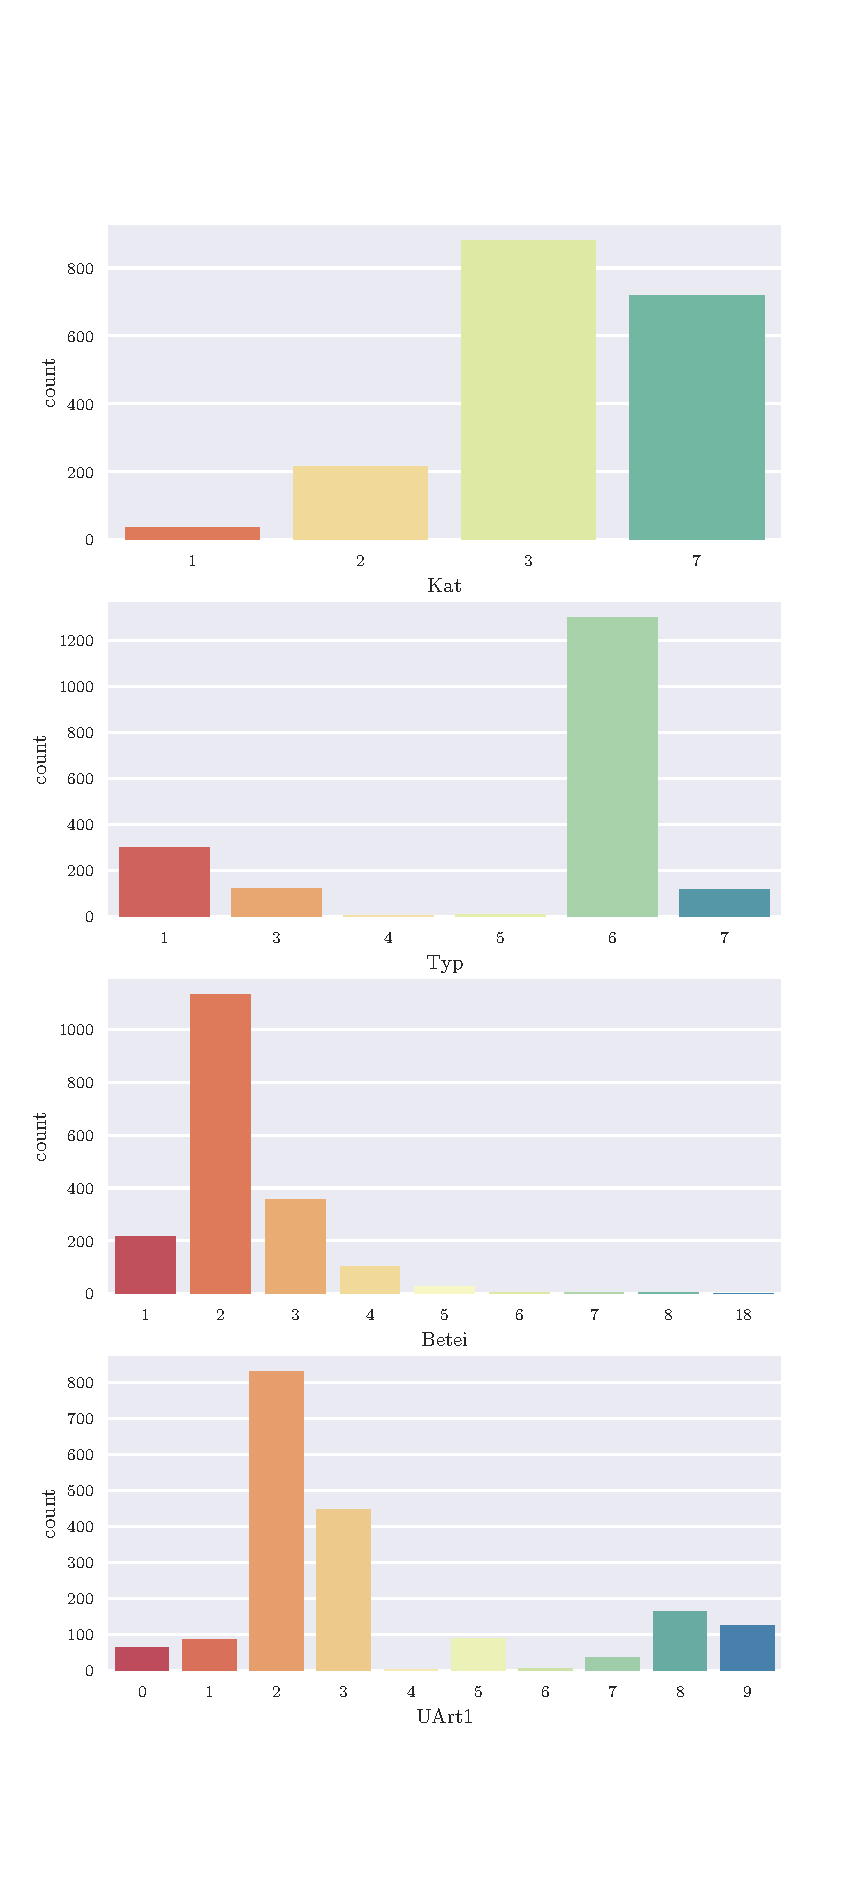
\includegraphics[scale=0.7]{CorrAnalysis/data/BAYSIS/02_matched/plots/baysis_matched_count_multiple01}
    %     \caption{Distribution of the accident category Kat, Typ, Betei and UArt}
    %     \label{img:baysis_matched_Kat}
    %     \label{img:baysis_matched_Typ}
    %     \label{img:baysis_matched_Betei}
    %     \label{img:baysis_matched_UArt}
    % \end{figure}

    % \begin{figure}[ht!]
    %     \centering
    %     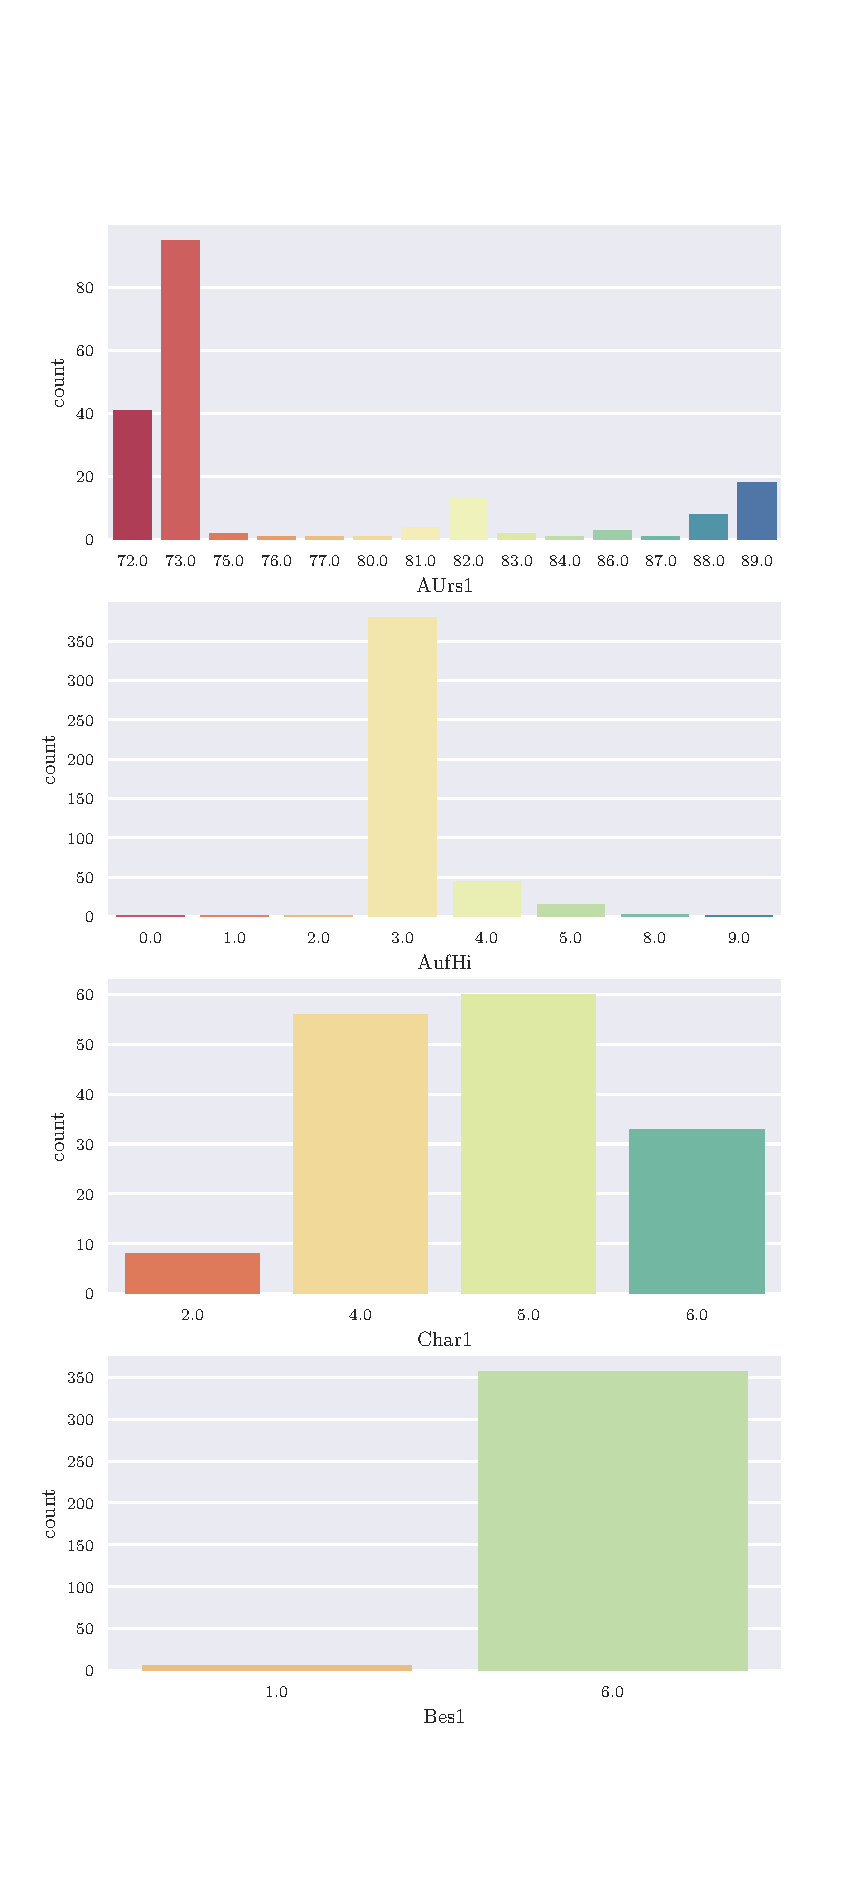
\includegraphics[scale=0.7]{CorrAnalysis/data/BAYSIS/02_matched/plots/baysis_matched_count_multiple02}
    %     \caption{Distribution of the accident category AUrs, AufHi, Char and Bes}
    %     \label{img:baysis_matched_AUrs}
    %     \label{img:baysis_matched_AufHi}
    %     \label{img:baysis_matched_Char}
    %     \label{img:baysis_matched_Bes}
    % \end{figure}

    % \begin{figure}[ht!]
    %     \centering
    %     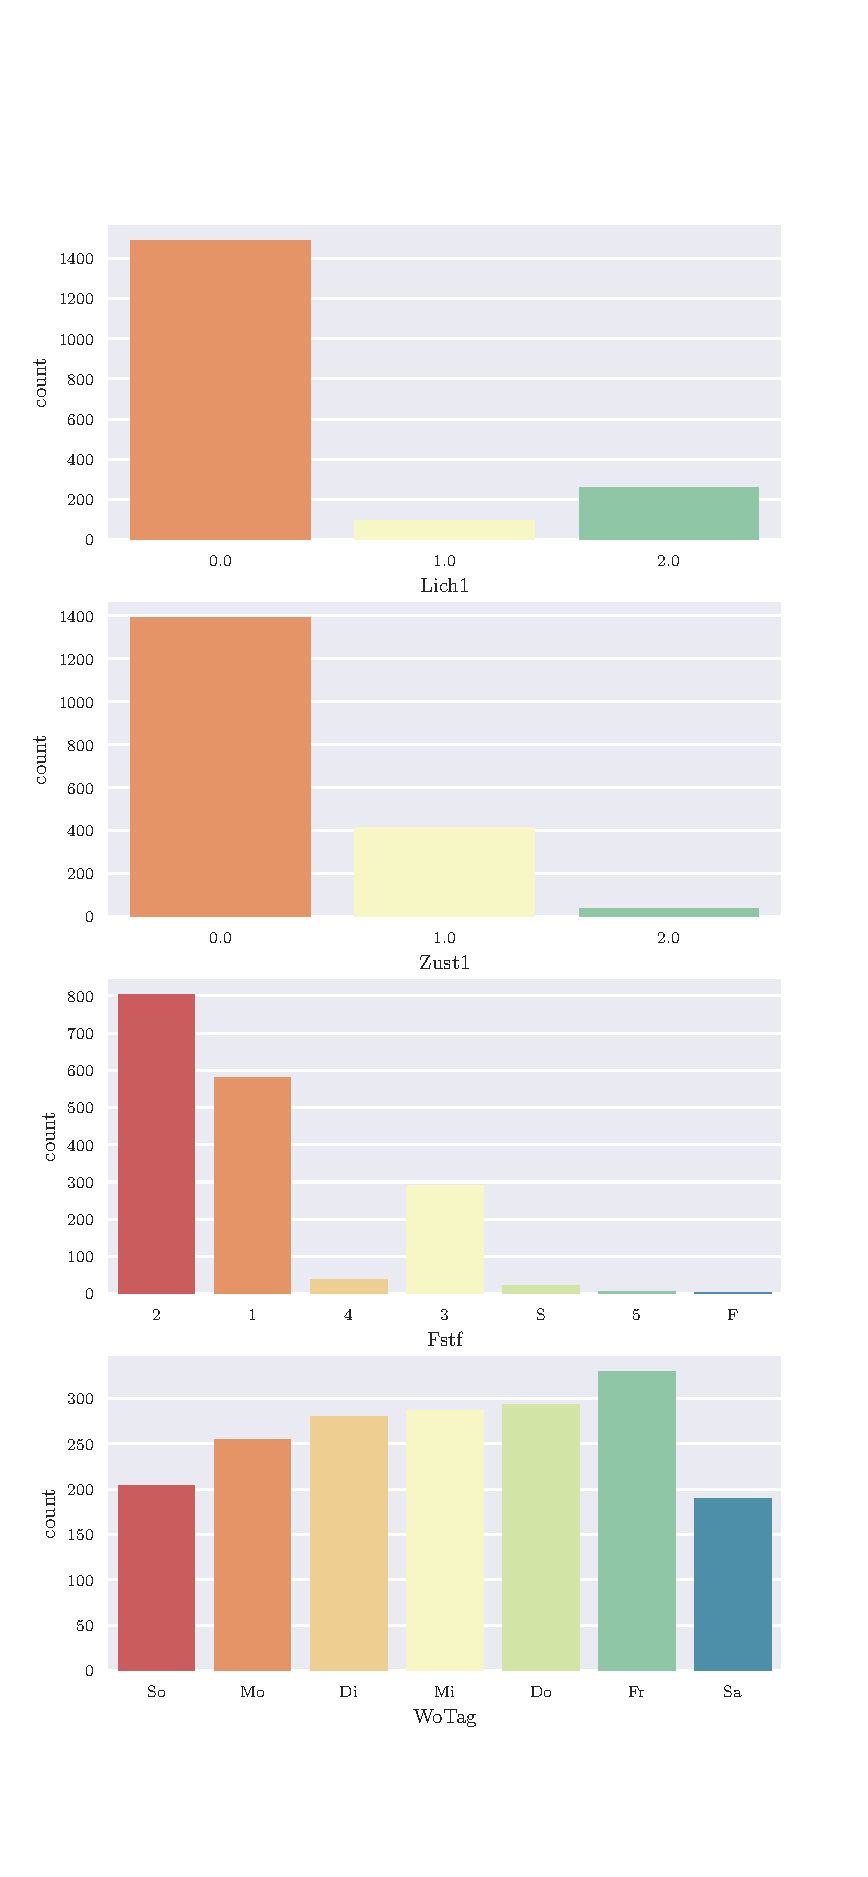
\includegraphics[scale=0.7]{CorrAnalysis/data/BAYSIS/02_matched/plots/baysis_matched_count_multiple03}
    %     \caption{Distribution of the accident category Lich, Zust, Fstf and WoTag}
    %     \label{img:baysis_matched_Lich}
    %     \label{img:baysis_matched_Zust}
    %     \label{img:baysis_matched_Fstf}
    %     \label{img:baysis_matched_WoTag}
    % \end{figure}

    \begin{table}[ht!]
        \tiny
        \centering
        \begin{tabular}{rrrrrr}
            \toprule
            & 1 & 3 & 4 & 5 & 6 \\ 
            \midrule
            3 & \red{0.05} &  &  &  &  \\ 
            4 & 1.00 & 0.38 &  &  &  \\ 
            5 & 0.96 & 1.00 & 0.96 &  &  \\ 
            6 & \red{0.00} & 0.96 & 0.51 & 1.00 &  \\ 
            7 & 1.00 & \red{0.04} & 1.00 & 0.96 & \red{0.01} \\ 
            \bottomrule
        \end{tabular}
        \caption{Pairwise Wilcoxon $T$-test for \textit{Typ} and \textit{Temporal Distance} (Jam Initiator) complete}
        \label{tbl:wilcoxon_baysis_initiator_Typ_TDist_complete}
    \end{table}
    
    % ------- BAYSIS Selected01 - Tables --------
    % \newgeometry{left=1cm,right=1cm,bottom=2cm}
    \begin{sidewaystable}
    	\tiny
    	\setlength{\tabcolsep}{2pt}
    	\centering
    	\begin{tabular}{lrrrrrrrrrrrrrrrrrrrrrrrrrrrrr}
\toprule
{} &  TMax &  TAvg &  SMax &  SAvg &  TDist &  SDist &   Cov &  TLCar &  TLHGV &  Str &  Kat &  Typ &  Betei &  UArt1 &  UArt2 &  AUrs1 &  AUrs2 &  AufHi &  Alkoh &  Char1 &  Char2 &  Lich1 &  Lich2 &  Zust1 &  Zust2 &  Fstf &  WoTag &  FeiTag &  Month \\
\midrule
TMax   &  1.00 &  0.89 &  0.60 &  0.53 &  -0.11 &  -0.03 & -0.21 &   0.02 &  -0.00 & 0.18 & 0.29 & 0.06 &   0.14 &   0.16 &   0.05 &   0.23 &   0.15 &   0.16 &   0.00 &   0.05 &   0.04 &   0.02 &   0.02 &   0.10 &   0.10 &  0.03 &   0.07 &   -0.02 &   0.12 \\
TAvg   &  0.89 &  1.00 &  0.39 &  0.55 &  -0.09 &  -0.03 &  0.08 &   0.01 &  -0.01 & 0.15 & 0.27 & 0.11 &   0.09 &   0.20 &   0.07 &   0.21 &   0.20 &   0.14 &   0.02 &   0.04 &   0.04 &   0.04 &   0.01 &   0.08 &   0.16 &  0.03 &   0.10 &   -0.01 &   0.11 \\
SMax   &  0.60 &  0.39 &  1.00 &  0.72 &  -0.09 &  -0.01 & -0.46 &   0.02 &  -0.00 & 0.26 & 0.20 & 0.08 &   0.11 &   0.20 &   0.07 &   0.22 &   0.11 &   0.13 &  -0.06 &   0.09 &   0.06 &   0.13 &   0.08 &   0.10 &   0.07 &  0.03 &   0.08 &   -0.02 &   0.14 \\
SAvg   &  0.53 &  0.55 &  0.72 &  1.00 &  -0.01 &  -0.04 &  0.10 &   0.05 &  -0.04 & 0.24 & 0.26 & 0.16 &   0.08 &   0.27 &   0.06 &   0.25 &   0.19 &   0.09 &  -0.03 &   0.07 &   0.02 &   0.03 &   0.02 &   0.09 &   0.16 &  0.04 &   0.12 &    0.00 &   0.13 \\
TDist  & -0.11 & -0.09 & -0.09 & -0.01 &   1.00 &   0.03 &  0.13 &  -0.01 &   0.06 & 0.10 & 0.10 & 0.21 &  -0.13 &   0.24 &   0.03 &   0.22 &   0.15 &   0.14 &   0.07 &   0.14 &   0.12 &   0.18 &   0.17 &   0.13 &   0.01 &  0.05 &   0.10 &    0.00 &   0.11 \\
SDist  & -0.03 & -0.03 & -0.01 & -0.04 &   0.03 &   1.00 & -0.07 &  -0.00 &  -0.00 & 0.06 & 0.07 & 0.03 &  -0.02 &   0.07 &   0.02 &   0.02 &   0.00 &   0.03 &  -0.00 &   0.01 &   0.01 &   0.02 &   0.02 &   0.02 &   0.00 &  0.07 &   0.09 &   -0.01 &   0.11 \\
Cov    & -0.21 &  0.08 & -0.46 &  0.10 &   0.13 &  -0.07 &  1.00 &   0.02 &  -0.04 & 0.22 & 0.04 & 0.18 &  -0.07 &   0.19 &   0.06 &   0.25 &   0.13 &   0.14 &   0.08 &   0.11 &   0.07 &   0.12 &   0.09 &   0.18 &   0.04 &  0.03 &   0.13 &    0.03 &   0.16 \\
TLCar  &  0.02 &  0.01 &  0.02 &  0.05 &  -0.01 &  -0.00 &  0.02 &   1.00 &   0.02 & 0.18 & 0.03 & 0.10 &   0.02 &   0.15 &   0.10 &   0.12 &   0.09 &   0.07 &   0.01 &   0.08 &   0.04 &   0.04 &   0.04 &   0.06 &   0.01 &  0.03 &   0.07 &    0.03 &   0.09 \\
TLHGV  & -0.00 & -0.01 & -0.00 & -0.04 &   0.06 &  -0.00 & -0.04 &   0.02 &   1.00 & 0.13 & 0.09 & 0.08 &  -0.03 &   0.09 &   0.07 &   0.18 &   0.11 &   0.08 &   0.07 &   0.10 &   0.03 &   0.06 &   0.06 &   0.03 &   0.05 &  0.02 &   0.13 &    0.01 &   0.16 \\
Str    &  0.18 &  0.15 &  0.26 &  0.24 &   0.10 &   0.06 &  0.22 &   0.18 &   0.13 & 1.00 & 0.16 & 0.16 &   0.13 &   0.13 &   0.16 &   0.13 &   0.08 &   0.13 &   0.07 &   0.14 &   0.12 &   0.12 &   0.16 &   0.11 &   0.15 &  0.19 &   0.15 &    0.07 &   0.15 \\
Kat    &  0.29 &  0.27 &  0.20 &  0.26 &   0.10 &   0.07 &  0.04 &   0.03 &   0.09 & 0.16 & 1.00 & 0.20 &   0.17 &   0.31 &   0.14 &   0.18 &   0.09 &   0.20 &   0.05 &   0.13 &   0.10 &   0.09 &   0.10 &   0.12 &   0.09 &  0.11 &   0.09 &    0.03 &   0.14 \\
Typ    &  0.06 &  0.11 &  0.08 &  0.16 &   0.21 &   0.03 &  0.18 &   0.10 &   0.08 & 0.16 & 0.20 & 1.00 &   0.30 &   0.63 &   0.09 &   0.25 &   0.10 &   0.24 &   0.16 &   0.15 &   0.20 &   0.08 &   0.08 &   0.19 &   0.08 &  0.13 &   0.11 &    0.04 &   0.13 \\
Betei  &  0.14 &  0.09 &  0.11 &  0.08 &  -0.13 &  -0.02 & -0.07 &   0.02 &  -0.03 & 0.13 & 0.17 & 0.30 &   1.00 &   0.29 &   0.10 &   0.21 &   0.42 &   0.19 &   0.05 &   0.11 &   0.18 &   0.10 &   0.09 &   0.12 &   0.42 &  0.10 &   0.11 &    0.04 &   0.13 \\
UArt1  &  0.16 &  0.20 &  0.20 &  0.27 &   0.24 &   0.07 &  0.19 &   0.15 &   0.09 & 0.13 & 0.31 & 0.63 &   0.29 &   1.00 &   0.16 &   0.21 &   0.11 &   0.29 &   0.16 &   0.22 &   0.19 &   0.11 &   0.12 &   0.19 &   0.09 &  0.15 &   0.14 &    0.08 &   0.12 \\
UArt2  &  0.05 &  0.07 &  0.07 &  0.06 &   0.03 &   0.02 &  0.06 &   0.10 &   0.07 & 0.16 & 0.14 & 0.09 &   0.10 &   0.16 &   1.00 &   0.14 &   0.07 &   0.26 &   0.03 &   0.11 &   0.13 &   0.09 &   0.11 &   0.08 &   0.03 &  0.12 &   0.10 &    0.07 &   0.14 \\
AUrs1  &  0.23 &  0.21 &  0.22 &  0.25 &   0.22 &   0.02 &  0.25 &   0.12 &   0.18 & 0.13 & 0.18 & 0.25 &   0.21 &   0.21 &   0.14 &   1.00 &   0.45 &   0.13 &   0.05 &   0.15 &   0.20 &   0.11 &   0.11 &   0.49 &   0.59 &  0.08 &   0.12 &    0.06 &   0.16 \\
AUrs2  &  0.15 &  0.20 &  0.11 &  0.19 &   0.15 &   0.00 &  0.13 &   0.09 &   0.11 & 0.08 & 0.09 & 0.10 &   0.42 &   0.11 &   0.07 &   0.45 &   1.00 &   0.05 &   0.01 &   0.06 &   0.13 &   0.04 &   0.04 &   0.18 &   0.65 &  0.05 &   0.10 &    0.02 &   0.12 \\
AufHi  &  0.16 &  0.14 &  0.13 &  0.09 &   0.14 &   0.03 &  0.14 &   0.07 &   0.08 & 0.13 & 0.20 & 0.24 &   0.19 &   0.29 &   0.26 &   0.13 &   0.05 &   1.00 &   0.03 &   0.12 &   0.18 &   0.08 &   0.09 &   0.15 &   0.03 &  0.12 &   0.11 &    0.05 &   0.12 \\
Alkoh  &  0.00 &  0.02 & -0.06 & -0.03 &   0.07 &  -0.00 &  0.08 &   0.01 &   0.07 & 0.07 & 0.05 & 0.16 &   0.05 &   0.16 &   0.03 &   0.05 &   0.01 &   0.03 &   1.00 &   0.08 &   0.01 &   0.17 &   0.14 &   0.02 &   0.05 &  0.10 &   0.04 &    0.01 &   0.10 \\
Char1  &  0.05 &  0.04 &  0.09 &  0.07 &   0.14 &   0.01 &  0.11 &   0.08 &   0.10 & 0.14 & 0.13 & 0.15 &   0.11 &   0.22 &   0.11 &   0.15 &   0.06 &   0.12 &   0.08 &   1.00 &   0.62 &   0.07 &   0.09 &   0.10 &   0.04 &  0.08 &   0.09 &    0.06 &   0.12 \\
Char2  &  0.04 &  0.04 &  0.06 &  0.02 &   0.12 &   0.01 &  0.07 &   0.04 &   0.03 & 0.12 & 0.10 & 0.20 &   0.18 &   0.19 &   0.13 &   0.20 &   0.13 &   0.18 &   0.01 &   0.62 &   1.00 &   0.08 &   0.08 &   0.16 &   0.02 &  0.13 &   0.15 &    0.06 &   0.07 \\
Lich1  &  0.02 &  0.04 &  0.13 &  0.03 &   0.18 &   0.02 &  0.12 &   0.04 &   0.06 & 0.12 & 0.09 & 0.08 &   0.10 &   0.11 &   0.09 &   0.11 &   0.04 &   0.08 &   0.17 &   0.07 &   0.08 &   1.00 &   0.71 &   0.43 &   0.05 &  0.08 &   0.11 &    0.06 &   0.20 \\
Lich2  &  0.02 &  0.01 &  0.08 &  0.02 &   0.17 &   0.02 &  0.09 &   0.04 &   0.06 & 0.16 & 0.10 & 0.08 &   0.09 &   0.12 &   0.11 &   0.11 &   0.04 &   0.09 &   0.14 &   0.09 &   0.08 &   0.71 &   1.00 &   0.15 &   0.02 &  0.06 &   0.14 &    0.07 &   0.23 \\
Zust1  &  0.10 &  0.08 &  0.10 &  0.09 &   0.13 &   0.02 &  0.18 &   0.06 &   0.03 & 0.11 & 0.12 & 0.19 &   0.12 &   0.19 &   0.08 &   0.49 &   0.18 &   0.15 &   0.02 &   0.10 &   0.16 &   0.43 &   0.15 &   1.00 &   0.16 &  0.09 &   0.09 &    0.05 &   0.27 \\
Zust2  &  0.10 &  0.16 &  0.07 &  0.16 &   0.01 &   0.00 &  0.04 &   0.01 &   0.05 & 0.15 & 0.09 & 0.08 &   0.42 &   0.09 &   0.03 &   0.59 &   0.65 &   0.03 &   0.05 &   0.04 &   0.02 &   0.05 &   0.02 &   0.16 &   1.00 &  0.04 &   0.10 &    0.02 &   0.20 \\
Fstf   &  0.03 &  0.03 &  0.03 &  0.04 &   0.05 &   0.07 &  0.03 &   0.03 &   0.02 & 0.19 & 0.11 & 0.13 &   0.10 &   0.15 &   0.12 &   0.08 &   0.05 &   0.12 &   0.10 &   0.08 &   0.13 &   0.08 &   0.06 &   0.09 &   0.04 &  1.00 &   0.10 &    0.06 &   0.13 \\
WoTag  &  0.07 &  0.10 &  0.08 &  0.12 &   0.10 &   0.09 &  0.13 &   0.07 &   0.13 & 0.15 & 0.09 & 0.11 &   0.11 &   0.14 &   0.10 &   0.12 &   0.10 &   0.11 &   0.04 &   0.09 &   0.15 &   0.11 &   0.14 &   0.09 &   0.10 &  0.10 &   1.00 &    0.18 &   0.15 \\
FeiTag & -0.02 & -0.01 & -0.02 &  0.00 &   0.00 &  -0.01 &  0.03 &   0.03 &   0.01 & 0.07 & 0.03 & 0.04 &   0.04 &   0.08 &   0.07 &   0.06 &   0.02 &   0.05 &   0.01 &   0.06 &   0.06 &   0.06 &   0.07 &   0.05 &   0.02 &  0.06 &   0.18 &    1.00 &   0.21 \\
Month  &  0.12 &  0.11 &  0.14 &  0.13 &   0.11 &   0.11 &  0.16 &   0.09 &   0.16 & 0.15 & 0.14 & 0.13 &   0.13 &   0.12 &   0.14 &   0.16 &   0.12 &   0.12 &   0.10 &   0.12 &   0.07 &   0.20 &   0.23 &   0.27 &   0.20 &  0.13 &   0.15 &    0.21 &   1.00 \\
\bottomrule
\end{tabular}

    	\caption{Correlation matrix for BAYSIS selected data (Jam Initiator), calculated with Cramer's $V$, $\eta$, $\tau$, $r_{pq}$, $r$}
    	\label{table:appendix_correlation_matrix_selected_startJam_cramers}
    \end{sidewaystable}
    \begin{sidewaystable}
    	\tiny
    	\setlength{\tabcolsep}{2pt}
    	\centering
    	\begin{tabular}{lrrrrrrrrrrrrrrrrrrrrrrrrrrrrr}
\toprule
{} &  TMax &  TAvg &  SMax &  SAvg &  TDist &  SDist &   Cov &  TLCar &  TLHGV &  Str &  Kat &  Typ &  Betei &  UArt1 &  UArt2 &  AUrs1 &  AUrs2 &  AufHi &  Alkoh &  Char1 &  Char2 &  Lich1 &  Lich2 &  Zust1 &  Zust2 &  Fstf &  WoTag &  FeiTag &  Month \\
\midrule
TMax   &  1.00 &  0.89 &  0.60 &  0.53 &  -0.11 &  -0.03 & -0.21 &   0.02 &  -0.00 & 0.18 & 0.29 & 0.06 &   0.14 &   0.16 &   0.05 &   0.23 &   0.15 &   0.16 &   0.00 &   0.05 &   0.04 &   0.02 &   0.02 &   0.10 &   0.10 &  0.03 &   0.07 &   -0.02 &   0.12 \\
TAvg   &  0.89 &  1.00 &  0.39 &  0.55 &  -0.09 &  -0.03 &  0.08 &   0.01 &  -0.01 & 0.15 & 0.27 & 0.11 &   0.09 &   0.20 &   0.07 &   0.21 &   0.20 &   0.14 &   0.02 &   0.04 &   0.04 &   0.04 &   0.01 &   0.08 &   0.16 &  0.03 &   0.10 &   -0.01 &   0.11 \\
SMax   &  0.60 &  0.39 &  1.00 &  0.72 &  -0.09 &  -0.01 & -0.46 &   0.02 &  -0.00 & 0.26 & 0.20 & 0.08 &   0.11 &   0.20 &   0.07 &   0.22 &   0.11 &   0.13 &  -0.06 &   0.09 &   0.06 &   0.13 &   0.08 &   0.10 &   0.07 &  0.03 &   0.08 &   -0.02 &   0.14 \\
SAvg   &  0.53 &  0.55 &  0.72 &  1.00 &  -0.01 &  -0.04 &  0.10 &   0.05 &  -0.04 & 0.24 & 0.26 & 0.16 &   0.08 &   0.27 &   0.06 &   0.25 &   0.19 &   0.09 &  -0.03 &   0.07 &   0.02 &   0.03 &   0.02 &   0.09 &   0.16 &  0.04 &   0.12 &    0.00 &   0.13 \\
TDist  & -0.11 & -0.09 & -0.09 & -0.01 &   1.00 &   0.03 &  0.13 &  -0.01 &   0.06 & 0.10 & 0.10 & 0.21 &  -0.13 &   0.24 &   0.03 &   0.22 &   0.15 &   0.14 &   0.07 &   0.14 &   0.12 &   0.18 &   0.17 &   0.13 &   0.01 &  0.05 &   0.10 &    0.00 &   0.11 \\
SDist  & -0.03 & -0.03 & -0.01 & -0.04 &   0.03 &   1.00 & -0.07 &  -0.00 &  -0.00 & 0.06 & 0.07 & 0.03 &  -0.02 &   0.07 &   0.02 &   0.02 &   0.00 &   0.03 &  -0.00 &   0.01 &   0.01 &   0.02 &   0.02 &   0.02 &   0.00 &  0.07 &   0.09 &   -0.01 &   0.11 \\
Cov    & -0.21 &  0.08 & -0.46 &  0.10 &   0.13 &  -0.07 &  1.00 &   0.02 &  -0.04 & 0.22 & 0.04 & 0.18 &  -0.07 &   0.19 &   0.06 &   0.25 &   0.13 &   0.14 &   0.08 &   0.11 &   0.07 &   0.12 &   0.09 &   0.18 &   0.04 &  0.03 &   0.13 &    0.03 &   0.16 \\
TLCar  &  0.02 &  0.01 &  0.02 &  0.05 &  -0.01 &  -0.00 &  0.02 &   1.00 &   0.02 & 0.18 & 0.03 & 0.10 &   0.02 &   0.15 &   0.10 &   0.12 &   0.09 &   0.07 &   0.01 &   0.08 &   0.04 &   0.04 &   0.04 &   0.06 &   0.01 &  0.03 &   0.07 &    0.03 &   0.09 \\
TLHGV  & -0.00 & -0.01 & -0.00 & -0.04 &   0.06 &  -0.00 & -0.04 &   0.02 &   1.00 & 0.13 & 0.09 & 0.08 &  -0.03 &   0.09 &   0.07 &   0.18 &   0.11 &   0.08 &   0.07 &   0.10 &   0.03 &   0.06 &   0.06 &   0.03 &   0.05 &  0.02 &   0.13 &    0.01 &   0.16 \\
Str    &  0.18 &  0.15 &  0.26 &  0.24 &   0.10 &   0.06 &  0.22 &   0.18 &   0.13 & 1.00 & 0.02 & 0.03 &   0.03 &   0.03 &   0.03 &   0.03 &   0.01 &   0.02 &   0.00 &   0.02 &   0.00 &   0.01 &   0.01 &   0.01 &   0.00 &  0.06 &   0.03 &    0.00 &   0.05 \\
Kat    &  0.29 &  0.27 &  0.20 &  0.26 &   0.10 &   0.07 &  0.04 &   0.03 &   0.09 & 0.04 & 1.00 & 0.05 &   0.04 &   0.10 &   0.02 &   0.04 &   0.01 &   0.04 &   0.00 &   0.02 &   0.00 &   0.01 &   0.01 &   0.02 &   0.00 &  0.02 &   0.01 &    0.00 &   0.03 \\
Typ    &  0.06 &  0.11 &  0.08 &  0.16 &   0.21 &   0.03 &  0.18 &   0.10 &   0.08 & 0.06 & 0.05 & 1.00 &   0.22 &   0.37 &   0.02 &   0.12 &   0.02 &   0.15 &   0.01 &   0.03 &   0.02 &   0.01 &   0.01 &   0.05 &   0.00 &  0.03 &   0.03 &    0.00 &   0.04 \\
Betei  &  0.14 &  0.09 &  0.11 &  0.08 &  -0.13 &  -0.02 & -0.07 &   0.02 &  -0.03 & 0.05 & 0.03 & 0.16 &   1.00 &   0.23 &   0.02 &   0.07 &   0.02 &   0.11 &   0.00 &   0.02 &   0.01 &   0.01 &   0.01 &   0.02 &   0.01 &  0.02 &   0.03 &    0.00 &   0.04 \\
UArt1  &  0.16 &  0.20 &  0.20 &  0.27 &   0.24 &   0.07 &  0.19 &   0.15 &   0.09 & 0.04 & 0.07 & 0.22 &   0.18 &   1.00 &   0.05 &   0.07 &   0.01 &   0.22 &   0.00 &   0.03 &   0.01 &   0.01 &   0.01 &   0.03 &   0.00 &  0.04 &   0.04 &    0.00 &   0.04 \\
UArt2  &  0.05 &  0.07 &  0.07 &  0.06 &   0.03 &   0.02 &  0.06 &   0.10 &   0.07 & 0.07 & 0.03 & 0.03 &   0.04 &   0.11 &   1.00 &   0.04 &   0.01 &   0.30 &   0.00 &   0.02 &   0.01 &   0.01 &   0.01 &   0.01 &   0.00 &  0.05 &   0.04 &    0.00 &   0.08 \\
AUrs1  &  0.23 &  0.21 &  0.22 &  0.25 &   0.22 &   0.02 &  0.25 &   0.12 &   0.18 & 0.11 & 0.07 & 0.18 &   0.14 &   0.17 &   0.04 &   1.00 &   0.06 &   0.11 &   0.00 &   0.04 &   0.02 &   0.03 &   0.02 &   0.31 &   0.05 &  0.04 &   0.07 &    0.00 &   0.16 \\
AUrs2  &  0.15 &  0.20 &  0.11 &  0.19 &   0.15 &   0.00 &  0.13 &   0.09 &   0.11 & 0.19 & 0.13 & 0.22 &   0.30 &   0.23 &   0.12 &   0.52 &   1.00 &   0.11 &   0.00 &   0.04 &   0.04 &   0.04 &   0.04 &   0.23 &   0.26 &  0.12 &   0.26 &    0.00 &   0.30 \\
AufHi  &  0.16 &  0.14 &  0.13 &  0.09 &   0.14 &   0.03 &  0.14 &   0.07 &   0.08 & 0.06 & 0.04 & 0.17 &   0.16 &   0.41 &   0.27 &   0.08 &   0.01 &   1.00 &   0.00 &   0.03 &   0.02 &   0.01 &   0.01 &   0.04 &   0.00 &  0.04 &   0.05 &    0.00 &   0.06 \\
Alkoh  &  0.00 &  0.02 & -0.06 & -0.03 &   0.07 &  -0.00 &  0.08 &   0.01 &   0.07 & 0.04 & 0.02 & 0.07 &   0.03 &   0.09 &   0.01 &   0.02 &   0.00 &   0.01 &   1.00 &   0.04 &   0.01 &   0.14 &   0.10 &   0.01 &   0.00 &  0.08 &   0.01 &    0.01 &   0.09 \\
Char1  &  0.05 &  0.04 &  0.09 &  0.07 &   0.14 &   0.01 &  0.11 &   0.08 &   0.10 & 0.08 & 0.05 & 0.06 &   0.04 &   0.08 &   0.03 &   0.05 &   0.01 &   0.04 &   0.01 &   1.00 &   0.19 &   0.01 &   0.01 &   0.03 &   0.00 &  0.03 &   0.03 &    0.00 &   0.05 \\
Char2  &  0.04 &  0.04 &  0.06 &  0.02 &   0.12 &   0.01 &  0.07 &   0.04 &   0.03 & 0.06 & 0.03 & 0.10 &   0.07 &   0.10 &   0.04 &   0.08 &   0.02 &   0.09 &   0.00 &   0.61 &   1.00 &   0.02 &   0.02 &   0.06 &   0.00 &  0.05 &   0.06 &    0.01 &   0.02 \\
Lich1  &  0.02 &  0.04 &  0.13 &  0.03 &   0.18 &   0.02 &  0.12 &   0.04 &   0.06 & 0.03 & 0.01 & 0.01 &   0.02 &   0.02 &   0.02 &   0.02 &   0.00 &   0.02 &   0.01 &   0.01 &   0.00 &   1.00 &   0.79 &   0.05 &   0.00 &  0.01 &   0.02 &    0.00 &   0.07 \\
Lich2  &  0.02 &  0.01 &  0.08 &  0.02 &   0.17 &   0.02 &  0.09 &   0.04 &   0.06 & 0.04 & 0.02 & 0.01 &   0.02 &   0.02 &   0.02 &   0.02 &   0.00 &   0.01 &   0.01 &   0.01 &   0.01 &   0.94 &   1.00 &   0.04 &   0.00 &  0.01 &   0.03 &    0.00 &   0.08 \\
Zust1  &  0.10 &  0.08 &  0.10 &  0.09 &   0.13 &   0.02 &  0.18 &   0.06 &   0.03 & 0.03 & 0.03 & 0.07 &   0.03 &   0.06 &   0.01 &   0.28 &   0.02 &   0.05 &   0.00 &   0.02 &   0.01 &   0.05 &   0.03 &   1.00 &   0.02 &  0.02 &   0.02 &    0.00 &   0.10 \\
Zust2  &  0.10 &  0.16 &  0.07 &  0.16 &   0.01 &   0.00 &  0.04 &   0.01 &   0.05 & 0.17 & 0.08 & 0.06 &   0.24 &   0.07 &   0.02 &   0.68 &   0.37 &   0.01 &   0.00 &   0.02 &   0.01 &   0.04 &   0.01 &   0.23 &   1.00 &  0.02 &   0.09 &    0.01 &   0.28 \\
Fstf   &  0.03 &  0.03 &  0.03 &  0.04 &   0.05 &   0.07 &  0.03 &   0.03 &   0.02 & 0.09 & 0.01 & 0.03 &   0.02 &   0.05 &   0.03 &   0.02 &   0.01 &   0.02 &   0.00 &   0.01 &   0.01 &   0.01 &   0.00 &   0.01 &   0.00 &  1.00 &   0.02 &    0.00 &   0.04 \\
WoTag  &  0.07 &  0.10 &  0.08 &  0.12 &   0.10 &   0.09 &  0.13 &   0.07 &   0.13 & 0.04 & 0.01 & 0.02 &   0.02 &   0.03 &   0.02 &   0.02 &   0.01 &   0.02 &   0.00 &   0.01 &   0.01 &   0.01 &   0.01 &   0.01 &   0.00 &  0.01 &   1.00 &    0.01 &   0.03 \\
FeiTag & -0.02 & -0.01 & -0.02 &  0.00 &   0.00 &  -0.01 &  0.03 &   0.03 &   0.01 & 0.03 & 0.00 & 0.01 &   0.01 &   0.04 &   0.02 &   0.02 &   0.00 &   0.01 &   0.00 &   0.01 &   0.02 &   0.01 &   0.01 &   0.01 &   0.00 &  0.02 &   0.12 &    1.00 &   0.17 \\
Month  &  0.12 &  0.11 &  0.14 &  0.13 &   0.11 &   0.11 &  0.16 &   0.09 &   0.16 & 0.04 & 0.01 & 0.02 &   0.02 &   0.03 &   0.03 &   0.04 &   0.01 &   0.02 &   0.00 &   0.01 &   0.00 &   0.02 &   0.02 &   0.03 &   0.01 &  0.02 &   0.03 &    0.01 &   1.00 \\
\bottomrule
\end{tabular}

    	\caption{Correlation matrix for BAYSIS selected data (Jam Initiator), calculated with Theil's $U$, $\eta$, $\tau$, $r_{pq}$, $r$}
    	\label{table:appendix_correlation_matrix_selected_startJam_theils}
    \end{sidewaystable}
    \begin{sidewaystable}
    	\tiny
    	\setlength{\tabcolsep}{2pt}
    	\centering
    	\begin{tabular}{lrrrrrrrrrrrrrrrrrrrrrrrrrrrrr}
\toprule
{} &  TMax &  TAvg &  SMax &  SAvg &  TDist &  SDist &   Cov &  TLCar &  TLHGV &   Str &   Kat &   Typ &  Betei &  UArt1 &  UArt2 &  AUrs1 &  AUrs2 &  AufHi &  Alkoh &  Char1 &  Char2 &  Lich1 &  Lich2 &  Zust1 &  Zust2 &  Fstf &  WoTag &  FeiTag &  Month \\
\midrule
TMax   &   nan & 0.000 & 0.000 & 0.000 &  0.002 &  0.361 & 0.000 &  0.671 &  0.921 & 0.000 & 0.000 & 0.000 &  0.000 &  0.000 &  0.000 &  0.000 &  0.000 &  0.000 &  0.965 &  0.000 &  0.000 &  0.000 &  0.000 &  0.000 &  0.000 & 0.325 &  0.000 &   0.576 &  0.000 \\
TAvg   & 0.000 &   nan & 0.000 & 0.000 &  0.011 &  0.335 & 0.021 &  0.680 &  0.724 & 0.000 & 0.000 & 0.000 &  0.001 &  0.000 &  0.000 &  0.000 &  0.000 &  0.000 &  0.527 &  0.000 &  0.000 &  0.000 &  0.000 &  0.000 &  0.000 & 0.206 &  0.000 &   0.716 &  0.000 \\
SMax   & 0.000 & 0.000 &   nan & 0.000 &  0.016 &  0.869 & 0.000 &  0.549 &  0.978 & 0.000 & 0.000 & 0.000 &  0.000 &  0.000 &  0.000 &  0.000 &  0.000 &  0.000 &  0.113 &  0.000 &  0.000 &  0.000 &  0.000 &  0.000 &  0.000 & 0.346 &  0.000 &   0.588 &  0.000 \\
SAvg   & 0.000 & 0.000 & 0.000 &   nan &  0.742 &  0.273 & 0.004 &  0.171 &  0.288 & 0.000 & 0.000 & 0.000 &  0.002 &  0.000 &  0.000 &  0.000 &  0.000 &  0.000 &  0.470 &  0.000 &  0.000 &  0.000 &  0.000 &  0.000 &  0.000 & 0.197 &  0.000 &   0.952 &  0.000 \\
TDist  & 0.002 & 0.011 & 0.016 & 0.742 &    nan &  0.449 & 0.000 &  0.827 &  0.110 & 0.000 & 0.000 & 0.000 &  0.000 &  0.000 &  0.000 &  0.000 &  0.000 &  0.000 &  0.043 &  0.000 &  0.000 &  0.000 &  0.000 &  0.000 &  0.000 & 0.094 &  0.000 &   0.970 &  0.000 \\
SDist  & 0.361 & 0.335 & 0.869 & 0.273 &  0.449 &    nan & 0.061 &  0.946 &  0.903 & 0.000 & 0.000 & 0.000 &  0.615 &  0.000 &  0.000 &  0.000 &  0.130 &  0.000 &  0.901 &  0.000 &  0.000 &  0.000 &  0.000 &  0.000 &  0.000 & 0.043 &  0.000 &   0.757 &  0.000 \\
Cov    & 0.000 & 0.021 & 0.000 & 0.004 &  0.000 &  0.061 &   nan &  0.494 &  0.245 & 0.000 & 0.000 & 0.000 &  0.009 &  0.000 &  0.000 &  0.000 &  0.000 &  0.000 &  0.024 &  0.000 &  0.000 &  0.000 &  0.000 &  0.000 &  0.000 & 0.222 &  0.000 &   0.336 &  0.000 \\
TLCar  & 0.671 & 0.680 & 0.549 & 0.171 &  0.827 &  0.946 & 0.494 &    nan &  0.595 & 0.000 & 0.000 & 0.000 &  0.400 &  0.000 &  0.000 &  0.000 &  0.000 &  0.000 &  0.808 &  0.000 &  0.000 &  0.000 &  0.000 &  0.000 &  0.000 & 0.307 &  0.000 &   0.360 &  0.000 \\
TLHGV  & 0.921 & 0.724 & 0.978 & 0.288 &  0.110 &  0.903 & 0.245 &  0.595 &    nan & 0.000 & 0.000 & 0.000 &  0.317 &  0.000 &  0.000 &  0.000 &  0.000 &  0.000 &  0.043 &  0.000 &  0.000 &  0.000 &  0.000 &  0.000 &  0.000 & 0.427 &  0.000 &   0.862 &  0.000 \\
Str    & 0.000 & 0.000 & 0.000 & 0.000 &  0.000 &  0.000 & 0.000 &  0.000 &  0.000 &   nan & 0.040 & 0.022 &  0.812 &  0.808 &  0.015 &  0.714 &  1.000 &  0.612 &  0.995 &  0.229 &  0.699 &  0.748 &  0.106 &  0.914 &  0.187 & 0.000 &  0.113 &   0.995 &  0.013 \\
Kat    & 0.000 & 0.000 & 0.000 & 0.000 &  0.000 &  0.000 & 0.000 &  0.000 &  0.000 & 0.040 &   nan & 0.000 &  0.000 &  0.000 &  0.004 &  0.000 &  0.534 &  0.000 &  0.516 &  0.000 &  0.037 &  0.049 &  0.028 &  0.000 &  0.124 & 0.157 &  0.705 &   0.842 &  0.039 \\
Typ    & 0.000 & 0.000 & 0.000 & 0.000 &  0.000 &  0.000 & 0.000 &  0.000 &  0.000 & 0.022 & 0.000 &   nan &  0.000 &  0.000 &  0.621 &  0.000 &  0.169 &  0.000 &  0.002 &  0.000 &  0.000 &  0.591 &  0.440 &  0.000 &  0.433 & 0.002 &  0.076 &   0.931 &  0.240 \\
Betei  & 0.000 & 0.001 & 0.000 & 0.002 &  0.000 &  0.615 & 0.009 &  0.400 &  0.317 & 0.812 & 0.000 & 0.000 &    nan &  0.000 &  0.543 &  0.000 &  0.000 &  0.000 &  0.980 &  0.319 &  0.002 &  0.494 &  0.601 &  0.055 &  0.000 & 0.598 &  0.146 &   0.992 &  0.184 \\
UArt1  & 0.000 & 0.000 & 0.000 & 0.000 &  0.000 &  0.000 & 0.000 &  0.000 &  0.000 & 0.808 & 0.000 & 0.000 &  0.000 &    nan &  0.000 &  0.000 &  0.282 &  0.000 &  0.018 &  0.000 &  0.001 &  0.288 &  0.206 &  0.000 &  0.756 & 0.000 &  0.002 &   0.819 &  0.379 \\
UArt2  & 0.000 & 0.000 & 0.000 & 0.000 &  0.000 &  0.000 & 0.000 &  0.000 &  0.000 & 0.015 & 0.004 & 0.621 &  0.543 &  0.000 &    nan &  0.021 &  0.997 &  0.000 &  0.999 &  0.115 &  0.079 &  0.583 &  0.159 &  0.839 &  0.996 & 0.011 &  0.442 &   0.779 &  0.008 \\
AUrs1  & 0.000 & 0.000 & 0.000 & 0.000 &  0.000 &  0.000 & 0.000 &  0.000 &  0.000 & 0.714 & 0.000 & 0.000 &  0.000 &  0.000 &  0.021 &    nan &  0.000 &  0.161 &  0.999 &  0.013 &  0.003 &  0.770 &  0.772 &  0.000 &  0.000 & 1.000 &  0.453 &   0.998 &  0.000 \\
AUrs2  & 0.000 & 0.000 & 0.000 & 0.000 &  0.000 &  0.130 & 0.000 &  0.000 &  0.000 & 1.000 & 0.534 & 0.169 &  0.000 &  0.282 &  0.997 &  0.000 &    nan &  1.000 &  1.000 &  0.996 &  0.059 &  1.000 &  0.997 &  0.000 &  0.000 & 1.000 &  0.302 &   1.000 &  0.379 \\
AufHi  & 0.000 & 0.000 & 0.000 & 0.000 &  0.000 &  0.000 & 0.000 &  0.000 &  0.000 & 0.612 & 0.000 & 0.000 &  0.000 &  0.000 &  0.000 &  0.161 &  1.000 &    nan &  0.999 &  0.036 &  0.002 &  0.910 &  0.772 &  0.002 &  0.999 & 0.020 &  0.111 &   0.976 &  0.514 \\
Alkoh  & 0.965 & 0.527 & 0.113 & 0.470 &  0.043 &  0.901 & 0.024 &  0.808 &  0.043 & 0.995 & 0.516 & 0.002 &  0.980 &  0.018 &  0.999 &  0.999 &  1.000 &  0.999 &    nan &  0.296 &  0.887 &  0.000 &  0.001 &  0.961 &  0.198 & 0.304 &  0.994 &   0.779 &  0.720 \\
Char1  & 0.000 & 0.000 & 0.000 & 0.000 &  0.000 &  0.000 & 0.000 &  0.000 &  0.000 & 0.229 & 0.000 & 0.000 &  0.319 &  0.000 &  0.115 &  0.013 &  0.996 &  0.036 &  0.296 &    nan &  0.000 &  0.384 &  0.141 &  0.026 &  0.908 & 0.907 &  0.543 &   0.654 &  0.512 \\
Char2  & 0.000 & 0.000 & 0.000 & 0.000 &  0.000 &  0.000 & 0.000 &  0.000 &  0.000 & 0.699 & 0.037 & 0.000 &  0.002 &  0.001 &  0.079 &  0.003 &  0.059 &  0.002 &  0.887 &  0.000 &    nan &  0.150 &  0.079 &  0.000 &  0.633 & 0.084 &  0.011 &   0.080 &  0.969 \\
Lich1  & 0.000 & 0.000 & 0.000 & 0.000 &  0.000 &  0.000 & 0.000 &  0.000 &  0.000 & 0.748 & 0.049 & 0.591 &  0.494 &  0.288 &  0.583 &  0.770 &  1.000 &  0.910 &  0.000 &  0.384 &  0.150 &    nan &  0.000 &  0.000 &  0.560 & 0.809 &  0.214 &   0.486 &  0.000 \\
Lich2  & 0.000 & 0.000 & 0.000 & 0.000 &  0.000 &  0.000 & 0.000 &  0.000 &  0.000 & 0.106 & 0.028 & 0.440 &  0.601 &  0.206 &  0.159 &  0.772 &  0.997 &  0.772 &  0.001 &  0.141 &  0.079 &  0.000 &    nan &  0.000 &  0.797 & 0.966 &  0.004 &   0.115 &  0.000 \\
Zust1  & 0.000 & 0.000 & 0.000 & 0.000 &  0.000 &  0.000 & 0.000 &  0.000 &  0.000 & 0.914 & 0.000 & 0.000 &  0.055 &  0.000 &  0.839 &  0.000 &  0.000 &  0.002 &  0.961 &  0.026 &  0.000 &  0.000 &  0.000 &    nan &  0.000 & 0.703 &  0.603 &   0.588 &  0.000 \\
Zust2  & 0.000 & 0.000 & 0.000 & 0.000 &  0.000 &  0.000 & 0.000 &  0.000 &  0.000 & 0.187 & 0.124 & 0.433 &  0.000 &  0.756 &  0.996 &  0.000 &  0.000 &  0.999 &  0.198 &  0.908 &  0.633 &  0.560 &  0.797 &  0.000 &    nan & 0.990 &  0.417 &   0.534 &  0.001 \\
Fstf   & 0.325 & 0.206 & 0.346 & 0.197 &  0.094 &  0.043 & 0.222 &  0.307 &  0.427 & 0.000 & 0.157 & 0.002 &  0.598 &  0.000 &  0.011 &  1.000 &  1.000 &  0.020 &  0.304 &  0.907 &  0.084 &  0.809 &  0.966 &  0.703 &  0.990 &   nan &  0.414 &   0.875 &  0.165 \\
WoTag  & 0.000 & 0.000 & 0.000 & 0.000 &  0.000 &  0.000 & 0.000 &  0.000 &  0.000 & 0.113 & 0.705 & 0.076 &  0.146 &  0.002 &  0.442 &  0.453 &  0.302 &  0.111 &  0.994 &  0.543 &  0.011 &  0.214 &  0.004 &  0.603 &  0.417 & 0.414 &    nan &   0.001 &  0.002 \\
FeiTag & 0.576 & 0.716 & 0.588 & 0.952 &  0.970 &  0.757 & 0.336 &  0.360 &  0.862 & 0.995 & 0.842 & 0.931 &  0.992 &  0.819 &  0.779 &  0.998 &  1.000 &  0.976 &  0.779 &  0.654 &  0.080 &  0.486 &  0.115 &  0.588 &  0.534 & 0.875 &  0.001 &     nan &  0.000 \\
Month  & 0.000 & 0.000 & 0.000 & 0.000 &  0.000 &  0.000 & 0.000 &  0.000 &  0.000 & 0.013 & 0.039 & 0.240 &  0.184 &  0.379 &  0.008 &  0.000 &  0.379 &  0.514 &  0.720 &  0.512 &  0.969 &  0.000 &  0.000 &  0.000 &  0.001 & 0.165 &  0.002 &   0.000 &    nan \\
\bottomrule
\end{tabular}

    	\caption{Significancy matrix for BAYSIS selected data (Jam Initiator)}
    	\label{table:appendix_significancy_matrix_selected_startJam}
    \end{sidewaystable}
    \begin{sidewaystable}
    	\tiny
    	\setlength{\tabcolsep}{2pt}
    	\centering
    	\begin{tabular}{llllllllllllllllllllllllllllll}
\toprule
{} &      TMax &      TAvg &      SMax &      SAvg &     TDist &     SDist &       Cov &     TLCar &     TLHGV &     Str &     Kat &     Typ &   Betei &   UArt1 &   UArt2 &   AUrs1 &   AUrs2 &   AufHi &     Alkoh &   Char1 &   Char2 &   Lich1 &   Lich2 &   Zust1 &   Zust2 &    Fstf &   WoTag &  FeiTag &   Month \\
\midrule
TMax   &       NaN &       $r$ &       $r$ &       $r$ &       $r$ &       $r$ &       $r$ &       $r$ &       $r$ &  $\eta$ &  $\eta$ &  $\eta$ &  $\tau$ &  $\eta$ &  $\eta$ &  $\eta$ &  $\eta$ &  $\eta$ &  $r_{pq}$ &  $\eta$ &  $\eta$ &  $\eta$ &  $\eta$ &  $\eta$ &  $\eta$ &  $\tau$ &  $\eta$ &  $\tau$ &  $\eta$ \\
TAvg   &       $r$ &       NaN &       $r$ &       $r$ &       $r$ &       $r$ &       $r$ &       $r$ &       $r$ &  $\eta$ &  $\eta$ &  $\eta$ &  $\tau$ &  $\eta$ &  $\eta$ &  $\eta$ &  $\eta$ &  $\eta$ &  $r_{pq}$ &  $\eta$ &  $\eta$ &  $\eta$ &  $\eta$ &  $\eta$ &  $\eta$ &  $\tau$ &  $\eta$ &  $\tau$ &  $\eta$ \\
SMax   &       $r$ &       $r$ &       NaN &       $r$ &       $r$ &       $r$ &       $r$ &       $r$ &       $r$ &  $\eta$ &  $\eta$ &  $\eta$ &  $\tau$ &  $\eta$ &  $\eta$ &  $\eta$ &  $\eta$ &  $\eta$ &  $r_{pq}$ &  $\eta$ &  $\eta$ &  $\eta$ &  $\eta$ &  $\eta$ &  $\eta$ &  $\tau$ &  $\eta$ &  $\tau$ &  $\eta$ \\
SAvg   &       $r$ &       $r$ &       $r$ &       NaN &       $r$ &       $r$ &       $r$ &       $r$ &       $r$ &  $\eta$ &  $\eta$ &  $\eta$ &  $\tau$ &  $\eta$ &  $\eta$ &  $\eta$ &  $\eta$ &  $\eta$ &  $r_{pq}$ &  $\eta$ &  $\eta$ &  $\eta$ &  $\eta$ &  $\eta$ &  $\eta$ &  $\tau$ &  $\eta$ &  $\tau$ &  $\eta$ \\
TDist  &       $r$ &       $r$ &       $r$ &       $r$ &       NaN &       $r$ &       $r$ &       $r$ &       $r$ &  $\eta$ &  $\eta$ &  $\eta$ &  $\tau$ &  $\eta$ &  $\eta$ &  $\eta$ &  $\eta$ &  $\eta$ &  $r_{pq}$ &  $\eta$ &  $\eta$ &  $\eta$ &  $\eta$ &  $\eta$ &  $\eta$ &  $\tau$ &  $\eta$ &  $\tau$ &  $\eta$ \\
SDist  &       $r$ &       $r$ &       $r$ &       $r$ &       $r$ &       NaN &       $r$ &       $r$ &       $r$ &  $\eta$ &  $\eta$ &  $\eta$ &  $\tau$ &  $\eta$ &  $\eta$ &  $\eta$ &  $\eta$ &  $\eta$ &  $r_{pq}$ &  $\eta$ &  $\eta$ &  $\eta$ &  $\eta$ &  $\eta$ &  $\eta$ &  $\tau$ &  $\eta$ &  $\tau$ &  $\eta$ \\
Cov    &       $r$ &       $r$ &       $r$ &       $r$ &       $r$ &       $r$ &       NaN &       $r$ &       $r$ &  $\eta$ &  $\eta$ &  $\eta$ &  $\tau$ &  $\eta$ &  $\eta$ &  $\eta$ &  $\eta$ &  $\eta$ &  $r_{pq}$ &  $\eta$ &  $\eta$ &  $\eta$ &  $\eta$ &  $\eta$ &  $\eta$ &  $\tau$ &  $\eta$ &  $\tau$ &  $\eta$ \\
TLCar  &       $r$ &       $r$ &       $r$ &       $r$ &       $r$ &       $r$ &       $r$ &       NaN &       $r$ &  $\eta$ &  $\eta$ &  $\eta$ &  $\tau$ &  $\eta$ &  $\eta$ &  $\eta$ &  $\eta$ &  $\eta$ &  $r_{pq}$ &  $\eta$ &  $\eta$ &  $\eta$ &  $\eta$ &  $\eta$ &  $\eta$ &  $\tau$ &  $\eta$ &  $\tau$ &  $\eta$ \\
TLHGV  &       $r$ &       $r$ &       $r$ &       $r$ &       $r$ &       $r$ &       $r$ &       $r$ &       NaN &  $\eta$ &  $\eta$ &  $\eta$ &  $\tau$ &  $\eta$ &  $\eta$ &  $\eta$ &  $\eta$ &  $\eta$ &  $r_{pq}$ &  $\eta$ &  $\eta$ &  $\eta$ &  $\eta$ &  $\eta$ &  $\eta$ &  $\tau$ &  $\eta$ &  $\tau$ &  $\eta$ \\
Str    &    $\eta$ &    $\eta$ &    $\eta$ &    $\eta$ &    $\eta$ &    $\eta$ &    $\eta$ &    $\eta$ &    $\eta$ &     NaN &     $V$ &     $V$ &     $V$ &     $V$ &     $V$ &     $V$ &     $V$ &     $V$ &       $V$ &     $V$ &     $V$ &     $V$ &     $V$ &     $V$ &     $V$ &     $V$ &     $V$ &     $V$ &     $V$ \\
Kat    &    $\eta$ &    $\eta$ &    $\eta$ &    $\eta$ &    $\eta$ &    $\eta$ &    $\eta$ &    $\eta$ &    $\eta$ &     $V$ &     NaN &     $V$ &     $V$ &     $V$ &     $V$ &     $V$ &     $V$ &     $V$ &       $V$ &     $V$ &     $V$ &     $V$ &     $V$ &     $V$ &     $V$ &     $V$ &     $V$ &     $V$ &     $V$ \\
Typ    &    $\eta$ &    $\eta$ &    $\eta$ &    $\eta$ &    $\eta$ &    $\eta$ &    $\eta$ &    $\eta$ &    $\eta$ &     $V$ &     $V$ &     NaN &     $V$ &     $V$ &     $V$ &     $V$ &     $V$ &     $V$ &       $V$ &     $V$ &     $V$ &     $V$ &     $V$ &     $V$ &     $V$ &     $V$ &     $V$ &     $V$ &     $V$ \\
Betei  &    $\tau$ &    $\tau$ &    $\tau$ &    $\tau$ &    $\tau$ &    $\tau$ &    $\tau$ &    $\tau$ &    $\tau$ &     $V$ &     $V$ &     $V$ &     NaN &     $V$ &     $V$ &     $V$ &     $V$ &     $V$ &       $V$ &     $V$ &     $V$ &     $V$ &     $V$ &     $V$ &     $V$ &     $V$ &     $V$ &     $V$ &     $V$ \\
UArt1  &    $\eta$ &    $\eta$ &    $\eta$ &    $\eta$ &    $\eta$ &    $\eta$ &    $\eta$ &    $\eta$ &    $\eta$ &     $V$ &     $V$ &     $V$ &     $V$ &     NaN &     $V$ &     $V$ &     $V$ &     $V$ &       $V$ &     $V$ &     $V$ &     $V$ &     $V$ &     $V$ &     $V$ &     $V$ &     $V$ &     $V$ &     $V$ \\
UArt2  &    $\eta$ &    $\eta$ &    $\eta$ &    $\eta$ &    $\eta$ &    $\eta$ &    $\eta$ &    $\eta$ &    $\eta$ &     $V$ &     $V$ &     $V$ &     $V$ &     $V$ &     NaN &     $V$ &     $V$ &     $V$ &       $V$ &     $V$ &     $V$ &     $V$ &     $V$ &     $V$ &     $V$ &     $V$ &     $V$ &     $V$ &     $V$ \\
AUrs1  &    $\eta$ &    $\eta$ &    $\eta$ &    $\eta$ &    $\eta$ &    $\eta$ &    $\eta$ &    $\eta$ &    $\eta$ &     $V$ &     $V$ &     $V$ &     $V$ &     $V$ &     $V$ &     NaN &     $V$ &     $V$ &       $V$ &     $V$ &     $V$ &     $V$ &     $V$ &     $V$ &     $V$ &     $V$ &     $V$ &     $V$ &     $V$ \\
AUrs2  &    $\eta$ &    $\eta$ &    $\eta$ &    $\eta$ &    $\eta$ &    $\eta$ &    $\eta$ &    $\eta$ &    $\eta$ &     $V$ &     $V$ &     $V$ &     $V$ &     $V$ &     $V$ &     $V$ &     NaN &     $V$ &       $V$ &     $V$ &     $V$ &     $V$ &     $V$ &     $V$ &     $V$ &     $V$ &     $V$ &     $V$ &     $V$ \\
AufHi  &    $\eta$ &    $\eta$ &    $\eta$ &    $\eta$ &    $\eta$ &    $\eta$ &    $\eta$ &    $\eta$ &    $\eta$ &     $V$ &     $V$ &     $V$ &     $V$ &     $V$ &     $V$ &     $V$ &     $V$ &     NaN &       $V$ &     $V$ &     $V$ &     $V$ &     $V$ &     $V$ &     $V$ &     $V$ &     $V$ &     $V$ &     $V$ \\
Alkoh  &  $r_{pq}$ &  $r_{pq}$ &  $r_{pq}$ &  $r_{pq}$ &  $r_{pq}$ &  $r_{pq}$ &  $r_{pq}$ &  $r_{pq}$ &  $r_{pq}$ &     $V$ &     $V$ &     $V$ &     $V$ &     $V$ &     $V$ &     $V$ &     $V$ &     $V$ &       NaN &     $V$ &     $V$ &     $V$ &     $V$ &     $V$ &     $V$ &     $V$ &     $V$ &     $V$ &     $V$ \\
Char1  &    $\eta$ &    $\eta$ &    $\eta$ &    $\eta$ &    $\eta$ &    $\eta$ &    $\eta$ &    $\eta$ &    $\eta$ &     $V$ &     $V$ &     $V$ &     $V$ &     $V$ &     $V$ &     $V$ &     $V$ &     $V$ &       $V$ &     NaN &     $V$ &     $V$ &     $V$ &     $V$ &     $V$ &     $V$ &     $V$ &     $V$ &     $V$ \\
Char2  &    $\eta$ &    $\eta$ &    $\eta$ &    $\eta$ &    $\eta$ &    $\eta$ &    $\eta$ &    $\eta$ &    $\eta$ &     $V$ &     $V$ &     $V$ &     $V$ &     $V$ &     $V$ &     $V$ &     $V$ &     $V$ &       $V$ &     $V$ &     NaN &     $V$ &     $V$ &     $V$ &     $V$ &     $V$ &     $V$ &     $V$ &     $V$ \\
Lich1  &    $\eta$ &    $\eta$ &    $\eta$ &    $\eta$ &    $\eta$ &    $\eta$ &    $\eta$ &    $\eta$ &    $\eta$ &     $V$ &     $V$ &     $V$ &     $V$ &     $V$ &     $V$ &     $V$ &     $V$ &     $V$ &       $V$ &     $V$ &     $V$ &     NaN &     $V$ &     $V$ &     $V$ &     $V$ &     $V$ &     $V$ &     $V$ \\
Lich2  &    $\eta$ &    $\eta$ &    $\eta$ &    $\eta$ &    $\eta$ &    $\eta$ &    $\eta$ &    $\eta$ &    $\eta$ &     $V$ &     $V$ &     $V$ &     $V$ &     $V$ &     $V$ &     $V$ &     $V$ &     $V$ &       $V$ &     $V$ &     $V$ &     $V$ &     NaN &     $V$ &     $V$ &     $V$ &     $V$ &     $V$ &     $V$ \\
Zust1  &    $\eta$ &    $\eta$ &    $\eta$ &    $\eta$ &    $\eta$ &    $\eta$ &    $\eta$ &    $\eta$ &    $\eta$ &     $V$ &     $V$ &     $V$ &     $V$ &     $V$ &     $V$ &     $V$ &     $V$ &     $V$ &       $V$ &     $V$ &     $V$ &     $V$ &     $V$ &     NaN &     $V$ &     $V$ &     $V$ &     $V$ &     $V$ \\
Zust2  &    $\eta$ &    $\eta$ &    $\eta$ &    $\eta$ &    $\eta$ &    $\eta$ &    $\eta$ &    $\eta$ &    $\eta$ &     $V$ &     $V$ &     $V$ &     $V$ &     $V$ &     $V$ &     $V$ &     $V$ &     $V$ &       $V$ &     $V$ &     $V$ &     $V$ &     $V$ &     $V$ &     NaN &     $V$ &     $V$ &     $V$ &     $V$ \\
Fstf   &    $\tau$ &    $\tau$ &    $\tau$ &    $\tau$ &    $\tau$ &    $\tau$ &    $\tau$ &    $\tau$ &    $\tau$ &     $V$ &     $V$ &     $V$ &     $V$ &     $V$ &     $V$ &     $V$ &     $V$ &     $V$ &       $V$ &     $V$ &     $V$ &     $V$ &     $V$ &     $V$ &     $V$ &     NaN &     $V$ &     $V$ &     $V$ \\
WoTag  &    $\eta$ &    $\eta$ &    $\eta$ &    $\eta$ &    $\eta$ &    $\eta$ &    $\eta$ &    $\eta$ &    $\eta$ &     $V$ &     $V$ &     $V$ &     $V$ &     $V$ &     $V$ &     $V$ &     $V$ &     $V$ &       $V$ &     $V$ &     $V$ &     $V$ &     $V$ &     $V$ &     $V$ &     $V$ &     NaN &     $V$ &     $V$ \\
FeiTag &    $\tau$ &    $\tau$ &    $\tau$ &    $\tau$ &    $\tau$ &    $\tau$ &    $\tau$ &    $\tau$ &    $\tau$ &     $V$ &     $V$ &     $V$ &     $V$ &     $V$ &     $V$ &     $V$ &     $V$ &     $V$ &       $V$ &     $V$ &     $V$ &     $V$ &     $V$ &     $V$ &     $V$ &     $V$ &     $V$ &     NaN &     $V$ \\
Month  &    $\eta$ &    $\eta$ &    $\eta$ &    $\eta$ &    $\eta$ &    $\eta$ &    $\eta$ &    $\eta$ &    $\eta$ &     $V$ &     $V$ &     $V$ &     $V$ &     $V$ &     $V$ &     $V$ &     $V$ &     $V$ &       $V$ &     $V$ &     $V$ &     $V$ &     $V$ &     $V$ &     $V$ &     $V$ &     $V$ &     $V$ &     NaN \\
\bottomrule
\end{tabular}

    	\caption{Coefficient matrix for BAYSIS selected data (Jam Initiator)}
    		\label{table:appendix_coefficient_matrix_selected_startJam}
    \end{sidewaystable}
    % \restoregeometry
    
    % -----------------------------------------------
    % ------- BAYSIS Selected02 - Jam Effector --------
    % -----------------------------------------------
    % \tocless\section{BAYSIS Selected Data - Jam Effector}
    % \label{appendix_baysis_selected_duringJam}
    
    % ------- BAYSIS Selected02 - Figures --------
    % \begin{figure}[ht!]
    %     \centering
    %     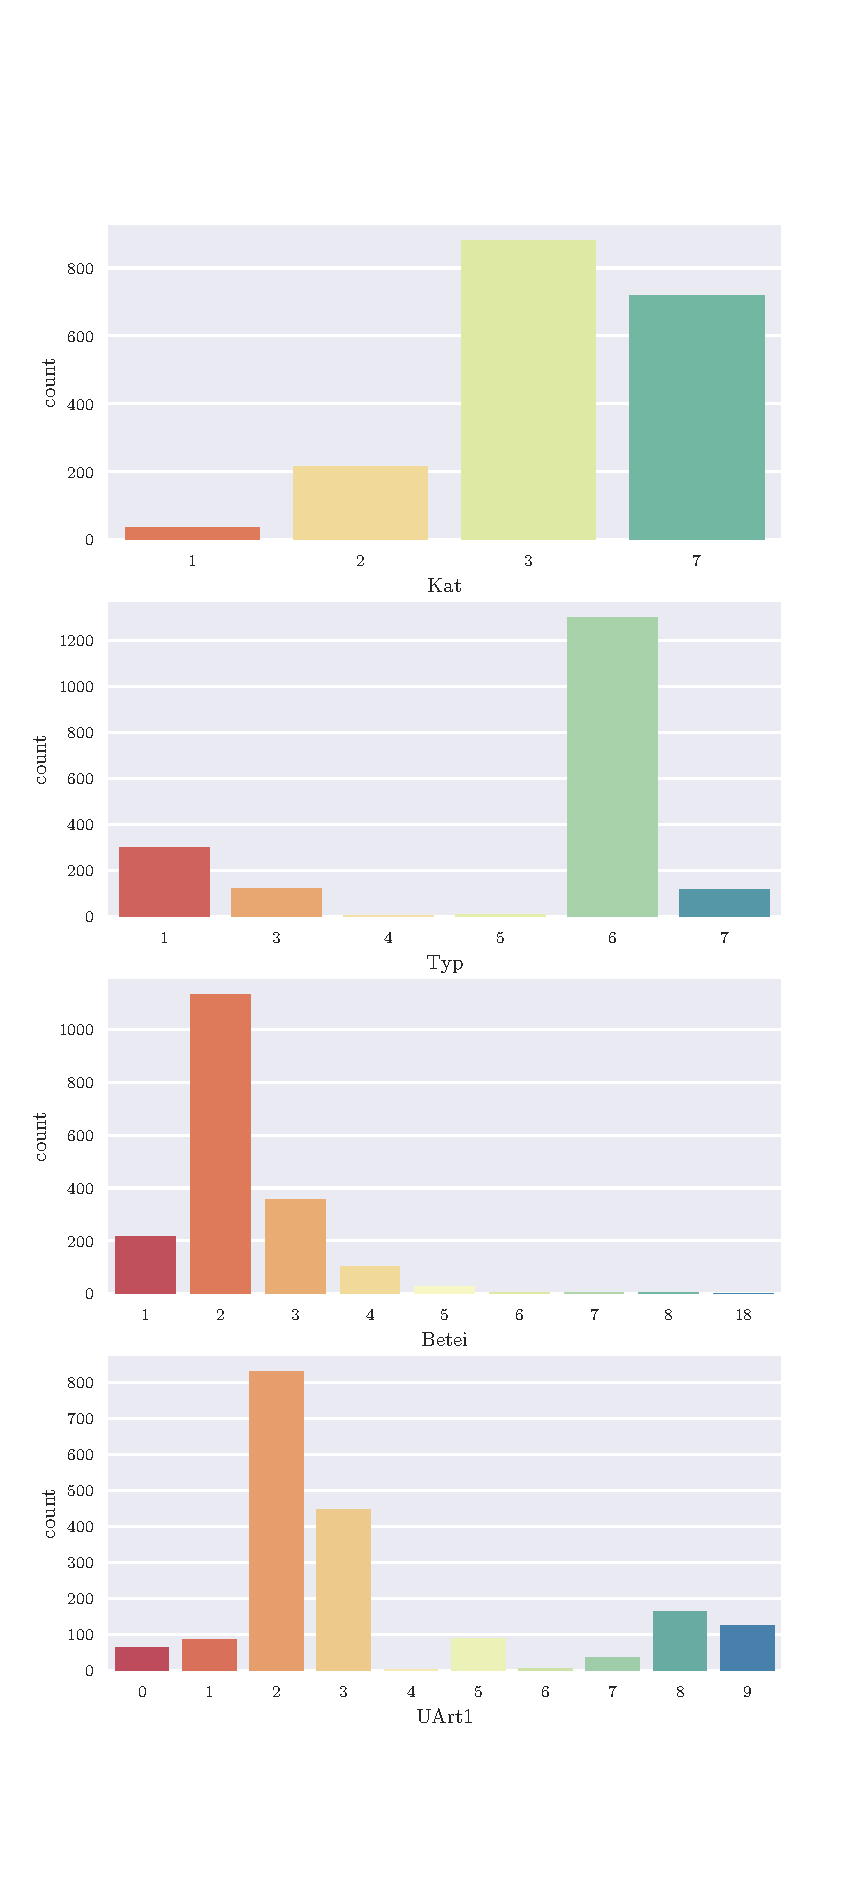
\includegraphics[scale=0.7]{CorrAnalysis/data/BAYSIS/02_matched/plots/baysis_matched_count_multiple01}
    %     \caption{Distribution of the accident category Kat, Typ, Betei and UArt}
    %     \label{img:baysis_matched_Kat}
    %     \label{img:baysis_matched_Typ}
    %     \label{img:baysis_matched_Betei}
    %     \label{img:baysis_matched_UArt}
    % \end{figure}

    % \begin{figure}[ht!]
    %     \centering
    %     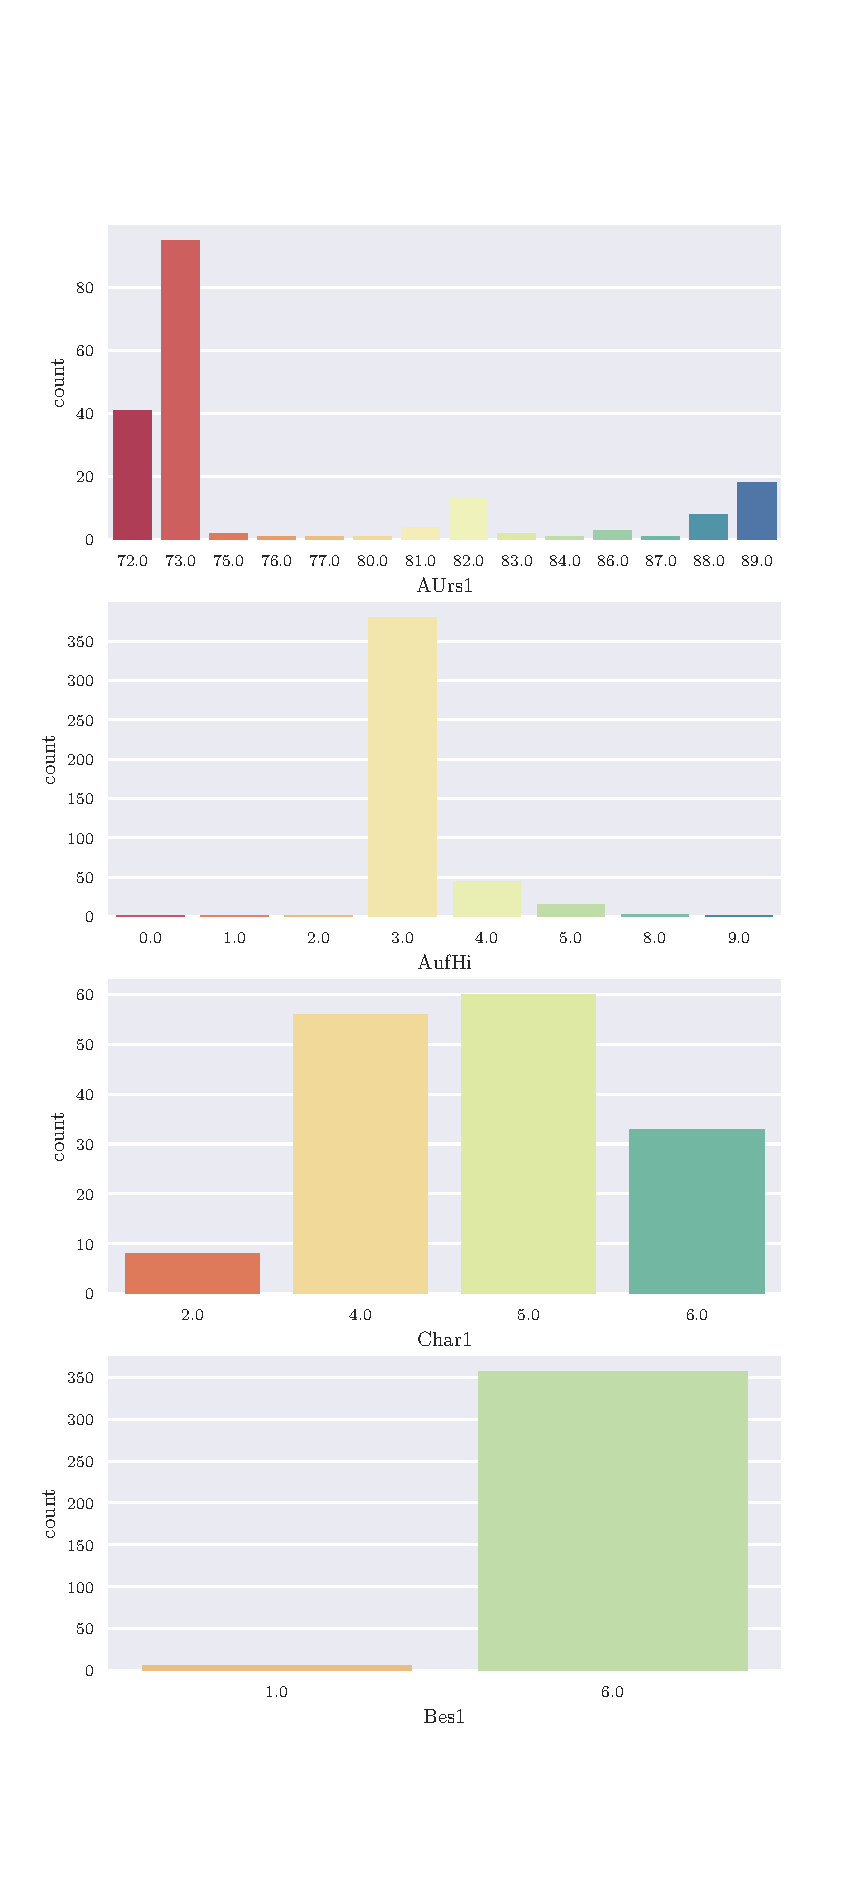
\includegraphics[scale=0.7]{CorrAnalysis/data/BAYSIS/02_matched/plots/baysis_matched_count_multiple02}
    %     \caption{Distribution of the accident category AUrs, AufHi, Char and Bes}
    %     \label{img:baysis_matched_AUrs}
    %     \label{img:baysis_matched_AufHi}
    %     \label{img:baysis_matched_Char}
    %     \label{img:baysis_matched_Bes}
    % \end{figure}

    % \begin{figure}[ht!]
    %     \centering
    %     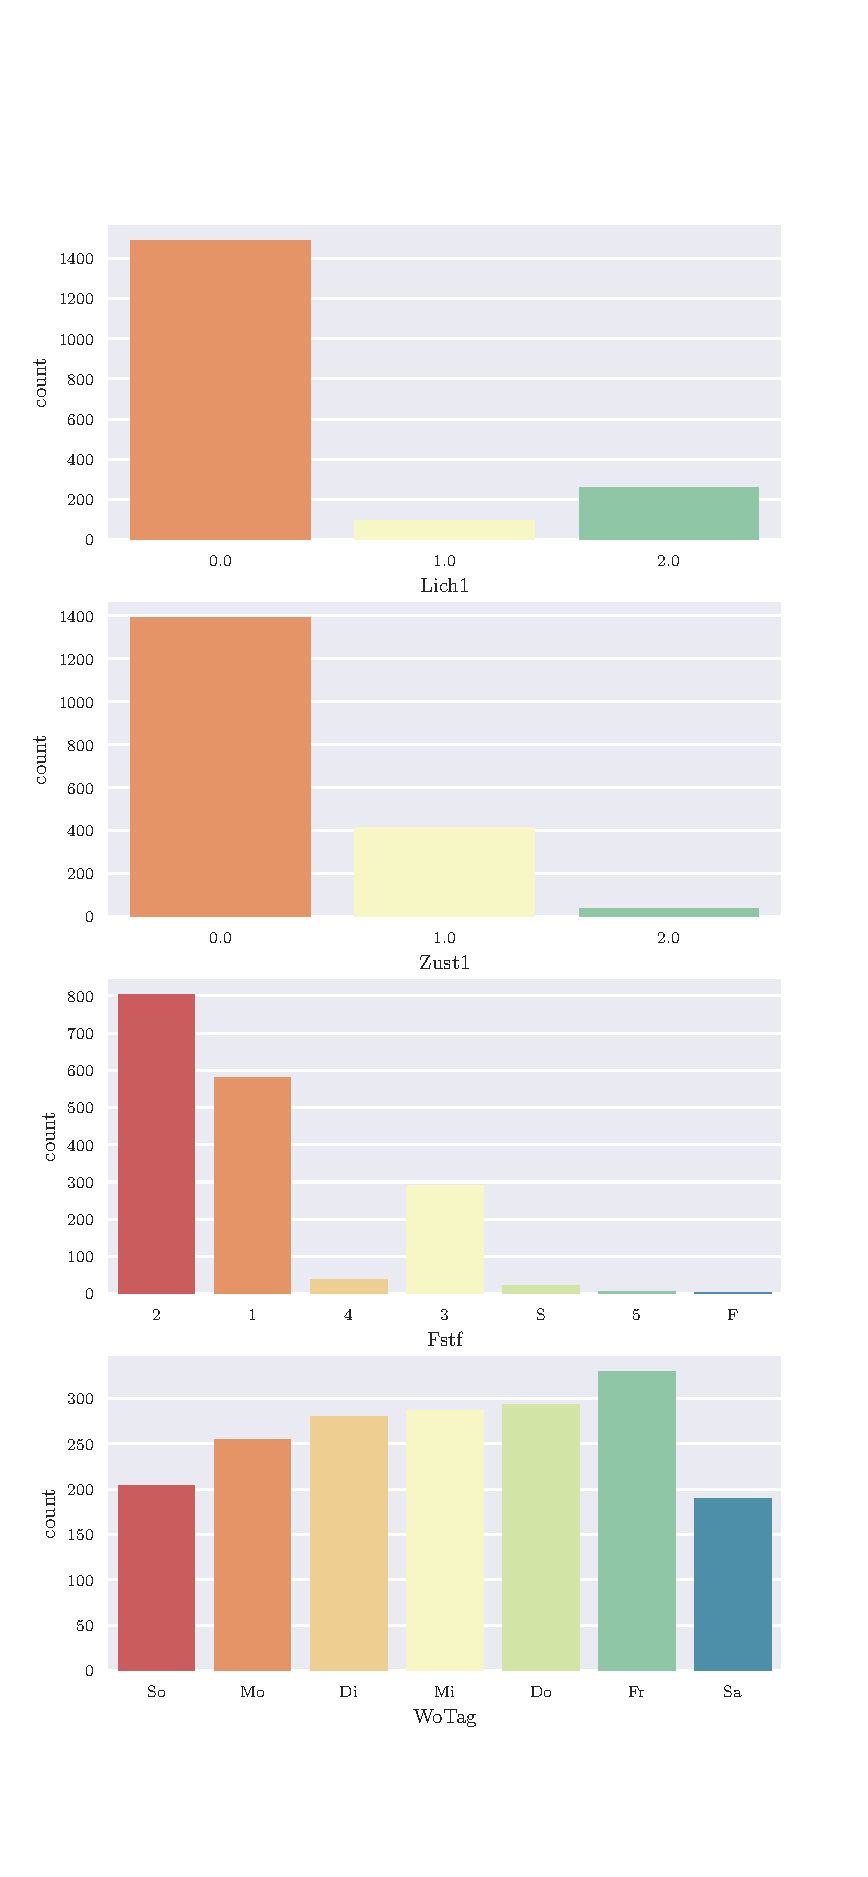
\includegraphics[scale=0.7]{CorrAnalysis/data/BAYSIS/02_matched/plots/baysis_matched_count_multiple03}
    %     \caption{Distribution of the accident category Lich, Zust, Fstf and WoTag}
    %     \label{img:baysis_matched_Lich}
    %     \label{img:baysis_matched_Zust}
    %     \label{img:baysis_matched_Fstf}
    %     \label{img:baysis_matched_WoTag}
    % \end{figure}
    
    % ------- BAYSIS Selected02 - Tables --------
    % \newgeometry{left=1cm,right=1cm,top=1cm}
    \begin{sidewaystable}
    	\tiny
    	\setlength{\tabcolsep}{2pt}
    	\centering
    	\begin{tabular}{lrrrrrrrrrrrrrrrrrrrrrrrrrrrrr}
\toprule
{} &  TMax &  TAvg &  SMax &  SAvg &  TDist &  SDist &   Cov &  TLCar &  TLHGV &  Str &  Kat &  Typ &  Betei &  UArt1 &  UArt2 &  AUrs1 &  AUrs2 &  AufHi &  Alkoh &  Char1 &  Char2 &  Lich1 &  Lich2 &  Zust1 &  Zust2 &  Fstf &  WoTag &  FeiTag &  Month \\
\midrule
TMax   &  1.00 &  0.80 &  0.50 &  0.43 &   0.00 &   0.00 & -0.19 &   0.03 &  -0.03 & 0.28 & 0.15 & 0.05 &   0.07 &   0.06 &   0.09 &   0.12 &   0.02 &   0.16 &  -0.02 &   0.09 &   0.05 &   0.05 &   0.05 &   0.11 &   0.03 &  0.00 &   0.12 &    0.03 &   0.19 \\
TAvg   &  0.80 &  1.00 &  0.22 &  0.46 &   0.00 &   0.00 &  0.18 &   0.03 &  -0.02 & 0.24 & 0.16 & 0.08 &   0.09 &   0.08 &   0.08 &   0.09 &   0.01 &   0.24 &   0.02 &   0.03 &   0.04 &   0.05 &   0.02 &   0.08 &   0.00 &  0.02 &   0.15 &    0.02 &   0.18 \\
SMax   &  0.50 &  0.22 &  1.00 &  0.62 &   0.00 &   0.00 & -0.48 &   0.00 &  -0.09 & 0.36 & 0.16 & 0.05 &   0.05 &   0.12 &   0.08 &   0.08 &   0.02 &   0.09 &  -0.05 &   0.10 &   0.02 &   0.06 &   0.05 &   0.08 &   0.05 &  0.06 &   0.11 &    0.07 &   0.19 \\
SAvg   &  0.43 &  0.46 &  0.62 &  1.00 &   0.00 &   0.00 &  0.18 &  -0.03 &  -0.10 & 0.31 & 0.24 & 0.04 &   0.10 &   0.17 &   0.10 &   0.13 &   0.03 &   0.04 &  -0.03 &   0.06 &   0.00 &   0.01 &   0.02 &   0.08 &   0.11 &  0.10 &   0.11 &    0.07 &   0.17 \\
TDist  &  0.00 &  0.00 &  0.00 &  0.00 &   0.00 &   0.00 &  0.00 &   0.00 &   0.00 & 0.00 & 0.00 & 0.00 &   0.00 &   0.00 &   0.00 &   0.00 &   0.00 &   0.00 &   0.00 &   0.00 &   0.00 &   0.00 &   0.00 &   0.00 &   0.00 &  0.00 &   0.00 &    0.00 &   0.00 \\
SDist  &  0.00 &  0.00 &  0.00 &  0.00 &   0.00 &   0.00 &  0.00 &   0.00 &   0.00 & 0.00 & 0.00 & 0.00 &   0.00 &   0.00 &   0.00 &   0.00 &   0.00 &   0.00 &   0.00 &   0.00 &   0.00 &   0.00 &   0.00 &   0.00 &   0.00 &  0.00 &   0.00 &    0.00 &   0.00 \\
Cov    & -0.19 &  0.18 & -0.48 &  0.18 &   0.00 &   0.00 &  1.00 &  -0.05 &   0.04 & 0.31 & 0.07 & 0.11 &   0.05 &   0.11 &   0.14 &   0.12 &   0.06 &   0.11 &   0.05 &   0.12 &   0.03 &   0.13 &   0.10 &   0.11 &   0.00 &  0.06 &   0.20 &   -0.01 &   0.19 \\
TLCar  &  0.03 &  0.03 &  0.00 & -0.03 &   0.00 &   0.00 & -0.05 &   1.00 &   0.00 & 0.12 & 0.01 & 0.11 &   0.00 &   0.11 &   0.10 &   0.12 &   0.03 &   0.05 &  -0.08 &   0.09 &   0.01 &   0.02 &   0.02 &   0.07 &   0.03 & -0.05 &   0.08 &   -0.04 &   0.10 \\
TLHGV  & -0.03 & -0.02 & -0.09 & -0.10 &   0.00 &   0.00 &  0.04 &   0.00 &   1.00 & 0.21 & 0.13 & 0.10 &   0.01 &   0.08 &   0.08 &   0.14 &   0.07 &   0.05 &  -0.05 &   0.12 &   0.01 &   0.03 &   0.03 &   0.11 &   0.05 & -0.01 &   0.14 &    0.05 &   0.21 \\
Str    &  0.28 &  0.24 &  0.36 &  0.31 &   0.00 &   0.00 &  0.31 &   0.12 &   0.21 & 1.00 & 0.14 & 0.15 &   0.12 &   0.20 &   0.15 &   0.14 &   0.11 &   0.12 &   0.08 &   0.22 &   0.15 &   0.18 &   0.16 &   0.22 &   0.14 &  0.18 &   0.16 &    0.12 &   0.15 \\
Kat    &  0.15 &  0.16 &  0.16 &  0.24 &   0.00 &   0.00 &  0.07 &   0.01 &   0.13 & 0.14 & 1.00 & 0.22 &   0.27 &   0.38 &   0.11 &   0.07 &   0.04 &   0.06 &   0.12 &   0.08 &   0.05 &   0.07 &   0.06 &   0.05 &   0.07 &  0.10 &   0.13 &    0.08 &   0.12 \\
Typ    &  0.05 &  0.08 &  0.05 &  0.04 &   0.00 &   0.00 &  0.11 &   0.11 &   0.10 & 0.15 & 0.22 & 1.00 &   0.32 &   0.51 &   0.10 &   0.27 &   0.08 &   0.25 &   0.07 &   0.14 &   0.13 &   0.12 &   0.13 &   0.16 &   0.26 &  0.14 &   0.13 &    0.08 &   0.15 \\
Betei  &  0.07 &  0.09 &  0.05 &  0.10 &   0.00 &   0.00 &  0.05 &   0.00 &   0.01 & 0.12 & 0.27 & 0.32 &   1.00 &   0.34 &   0.10 &   0.15 &   0.02 &   0.29 &   0.10 &   0.09 &   0.10 &   0.10 &   0.06 &   0.09 &   0.22 &  0.12 &   0.12 &    0.12 &   0.15 \\
UArt1  &  0.06 &  0.08 &  0.12 &  0.17 &   0.00 &   0.00 &  0.11 &   0.11 &   0.08 & 0.20 & 0.38 & 0.51 &   0.34 &   1.00 &   0.17 &   0.24 &   0.11 &   0.39 &   0.09 &   0.16 &   0.15 &   0.08 &   0.07 &   0.15 &   0.22 &  0.16 &   0.13 &    0.09 &   0.13 \\
UArt2  &  0.09 &  0.08 &  0.08 &  0.10 &   0.00 &   0.00 &  0.14 &   0.10 &   0.08 & 0.15 & 0.11 & 0.10 &   0.10 &   0.17 &   1.00 &   0.10 &   0.01 &   0.39 &   0.03 &   0.09 &   0.12 &   0.09 &   0.07 &   0.10 &   0.10 &  0.10 &   0.10 &    0.03 &   0.11 \\
AUrs1  &  0.12 &  0.09 &  0.08 &  0.13 &   0.00 &   0.00 &  0.12 &   0.12 &   0.14 & 0.14 & 0.07 & 0.27 &   0.15 &   0.24 &   0.10 &   1.00 &   0.28 &   0.30 &   0.03 &   0.07 &   0.02 &   0.10 &   0.08 &   0.42 &   0.52 &  0.05 &   0.10 &    0.06 &   0.18 \\
AUrs2  &  0.02 &  0.01 &  0.02 &  0.03 &   0.00 &   0.00 &  0.06 &   0.03 &   0.07 & 0.11 & 0.04 & 0.08 &   0.02 &   0.11 &   0.01 &   0.28 &   1.00 &   0.01 &   0.01 &   0.01 &   0.01 &   0.12 &   0.06 &   0.29 &   0.01 &  0.05 &   0.10 &    0.01 &   0.15 \\
AufHi  &  0.16 &  0.24 &  0.09 &  0.04 &   0.00 &   0.00 &  0.11 &   0.05 &   0.05 & 0.12 & 0.06 & 0.25 &   0.29 &   0.39 &   0.39 &   0.30 &   0.01 &   1.00 &   0.02 &   0.05 &   0.15 &   0.05 &   0.06 &   0.12 &   0.15 &  0.11 &   0.11 &    0.02 &   0.13 \\
Alkoh  & -0.02 &  0.02 & -0.05 & -0.03 &   0.00 &   0.00 &  0.05 &  -0.08 &  -0.05 & 0.08 & 0.12 & 0.07 &   0.10 &   0.09 &   0.03 &   0.03 &   0.01 &   0.02 &   1.00 &   0.09 &   0.05 &   0.14 &   0.14 &   0.08 &   0.05 &  0.04 &   0.08 &    0.02 &   0.09 \\
Char1  &  0.09 &  0.03 &  0.10 &  0.06 &   0.00 &   0.00 &  0.12 &   0.09 &   0.12 & 0.22 & 0.08 & 0.14 &   0.09 &   0.16 &   0.09 &   0.07 &   0.01 &   0.05 &   0.09 &   1.00 &   0.48 &   0.07 &   0.04 &   0.05 &   0.08 &  0.10 &   0.10 &    0.04 &   0.12 \\
Char2  &  0.05 &  0.04 &  0.02 &  0.00 &   0.00 &   0.00 &  0.03 &   0.01 &   0.01 & 0.15 & 0.05 & 0.13 &   0.10 &   0.15 &   0.12 &   0.02 &   0.01 &   0.15 &   0.05 &   0.48 &   1.00 &   0.06 &   0.04 &   0.03 &   0.06 &  0.08 &   0.10 &    0.04 &   0.12 \\
Lich1  &  0.05 &  0.05 &  0.06 &  0.01 &   0.00 &   0.00 &  0.13 &   0.02 &   0.03 & 0.18 & 0.07 & 0.12 &   0.10 &   0.08 &   0.09 &   0.10 &   0.12 &   0.05 &   0.14 &   0.07 &   0.06 &   1.00 &   0.71 &   0.13 &   0.05 &  0.09 &   0.12 &    0.03 &   0.32 \\
Lich2  &  0.05 &  0.02 &  0.05 &  0.02 &   0.00 &   0.00 &  0.10 &   0.02 &   0.03 & 0.16 & 0.06 & 0.13 &   0.06 &   0.07 &   0.07 &   0.08 &   0.06 &   0.06 &   0.14 &   0.04 &   0.04 &   0.71 &   1.00 &   0.13 &   0.04 &  0.09 &   0.11 &    0.01 &   0.32 \\
Zust1  &  0.11 &  0.08 &  0.08 &  0.08 &   0.00 &   0.00 &  0.11 &   0.07 &   0.11 & 0.22 & 0.05 & 0.16 &   0.09 &   0.15 &   0.10 &   0.42 &   0.29 &   0.12 &   0.08 &   0.05 &   0.03 &   0.13 &   0.13 &   1.00 &   0.22 &  0.07 &   0.11 &    0.05 &   0.27 \\
Zust2  &  0.03 &  0.00 &  0.05 &  0.11 &   0.00 &   0.00 &  0.00 &   0.03 &   0.05 & 0.14 & 0.07 & 0.26 &   0.22 &   0.22 &   0.10 &   0.52 &   0.01 &   0.15 &   0.05 &   0.08 &   0.06 &   0.05 &   0.04 &   0.22 &   1.00 &  0.08 &   0.10 &    0.04 &   0.25 \\
Fstf   &  0.00 &  0.02 &  0.06 &  0.10 &   0.00 &   0.00 &  0.06 &  -0.05 &  -0.01 & 0.18 & 0.10 & 0.14 &   0.12 &   0.16 &   0.10 &   0.05 &   0.05 &   0.11 &   0.04 &   0.10 &   0.08 &   0.09 &   0.09 &   0.07 &   0.08 &  1.00 &   0.10 &    0.13 &   0.13 \\
WoTag  &  0.12 &  0.15 &  0.11 &  0.11 &   0.00 &   0.00 &  0.20 &   0.08 &   0.14 & 0.16 & 0.13 & 0.13 &   0.12 &   0.13 &   0.10 &   0.10 &   0.10 &   0.11 &   0.08 &   0.10 &   0.10 &   0.12 &   0.11 &   0.11 &   0.10 &  0.10 &   1.00 &    0.14 &   0.16 \\
FeiTag &  0.03 &  0.02 &  0.07 &  0.07 &   0.00 &   0.00 & -0.01 &  -0.04 &   0.05 & 0.12 & 0.08 & 0.08 &   0.12 &   0.09 &   0.03 &   0.06 &   0.01 &   0.02 &   0.02 &   0.04 &   0.04 &   0.03 &   0.01 &   0.05 &   0.04 &  0.13 &   0.14 &    1.00 &   0.16 \\
Month  &  0.19 &  0.18 &  0.19 &  0.17 &   0.00 &   0.00 &  0.19 &   0.10 &   0.21 & 0.15 & 0.12 & 0.15 &   0.15 &   0.13 &   0.11 &   0.18 &   0.15 &   0.13 &   0.09 &   0.12 &   0.12 &   0.32 &   0.32 &   0.27 &   0.25 &  0.13 &   0.16 &    0.16 &   1.00 \\
\bottomrule
\end{tabular}

    	\caption{Correlation matrix for BAYSIS selected data (Jam Effector), calculated with Cramer's $V$, $\eta$, $\tau$, $r_{pq}$, $r$}
    	\label{table:appendix_correlation_matrix_selected_duringJam_cramers}
    \end{sidewaystable}  
    \begin{sidewaystable}
    	\tiny
    	\setlength{\tabcolsep}{2pt}
    	\centering
    	\begin{tabular}{lrrrrrrrrrrrrrrrrrrrrrrrrrrrrr}
\toprule
{} &  TMax &  TAvg &  SMax &  SAvg &  TDist &  SDist &   Cov &  TLCar &  TLHGV &  Str &  Kat &  Typ &  Betei &  UArt1 &  UArt2 &  AUrs1 &  AUrs2 &  AufHi &  Alkoh &  Char1 &  Char2 &  Lich1 &  Lich2 &  Zust1 &  Zust2 &  Fstf &  WoTag &  FeiTag &  Month \\
\midrule
TMax   &  1.00 &  0.80 &  0.50 &  0.43 &   0.00 &   0.00 & -0.19 &   0.03 &  -0.03 & 0.28 & 0.15 & 0.05 &   0.07 &   0.06 &   0.09 &   0.12 &   0.02 &   0.16 &  -0.02 &   0.09 &   0.05 &   0.05 &   0.05 &   0.11 &   0.03 &  0.00 &   0.12 &    0.03 &   0.19 \\
TAvg   &  0.80 &  1.00 &  0.22 &  0.46 &   0.00 &   0.00 &  0.18 &   0.03 &  -0.02 & 0.24 & 0.16 & 0.08 &   0.09 &   0.08 &   0.08 &   0.09 &   0.01 &   0.24 &   0.02 &   0.03 &   0.04 &   0.05 &   0.02 &   0.08 &   0.00 &  0.02 &   0.15 &    0.02 &   0.18 \\
SMax   &  0.50 &  0.22 &  1.00 &  0.62 &   0.00 &   0.00 & -0.48 &   0.00 &  -0.09 & 0.36 & 0.16 & 0.05 &   0.05 &   0.12 &   0.08 &   0.08 &   0.02 &   0.09 &  -0.05 &   0.10 &   0.02 &   0.06 &   0.05 &   0.08 &   0.05 &  0.06 &   0.11 &    0.07 &   0.19 \\
SAvg   &  0.43 &  0.46 &  0.62 &  1.00 &   0.00 &   0.00 &  0.18 &  -0.03 &  -0.10 & 0.31 & 0.24 & 0.04 &   0.10 &   0.17 &   0.10 &   0.13 &   0.03 &   0.04 &  -0.03 &   0.06 &   0.00 &   0.01 &   0.02 &   0.08 &   0.11 &  0.10 &   0.11 &    0.07 &   0.17 \\
TDist  &  0.00 &  0.00 &  0.00 &  0.00 &   0.00 &   0.00 &  0.00 &   0.00 &   0.00 & 0.00 & 0.00 & 0.00 &   0.00 &   0.00 &   0.00 &   0.00 &   0.00 &   0.00 &   0.00 &   0.00 &   0.00 &   0.00 &   0.00 &   0.00 &   0.00 &  0.00 &   0.00 &    0.00 &   0.00 \\
SDist  &  0.00 &  0.00 &  0.00 &  0.00 &   0.00 &   0.00 &  0.00 &   0.00 &   0.00 & 0.00 & 0.00 & 0.00 &   0.00 &   0.00 &   0.00 &   0.00 &   0.00 &   0.00 &   0.00 &   0.00 &   0.00 &   0.00 &   0.00 &   0.00 &   0.00 &  0.00 &   0.00 &    0.00 &   0.00 \\
Cov    & -0.19 &  0.18 & -0.48 &  0.18 &   0.00 &   0.00 &  1.00 &  -0.05 &   0.04 & 0.31 & 0.07 & 0.11 &   0.05 &   0.11 &   0.14 &   0.12 &   0.06 &   0.11 &   0.05 &   0.12 &   0.03 &   0.13 &   0.10 &   0.11 &   0.00 &  0.06 &   0.20 &   -0.01 &   0.19 \\
TLCar  &  0.03 &  0.03 &  0.00 & -0.03 &   0.00 &   0.00 & -0.05 &   1.00 &   0.00 & 0.12 & 0.01 & 0.11 &   0.00 &   0.11 &   0.10 &   0.12 &   0.03 &   0.05 &  -0.08 &   0.09 &   0.01 &   0.02 &   0.02 &   0.07 &   0.03 & -0.05 &   0.08 &   -0.04 &   0.10 \\
TLHGV  & -0.03 & -0.02 & -0.09 & -0.10 &   0.00 &   0.00 &  0.04 &   0.00 &   1.00 & 0.21 & 0.13 & 0.10 &   0.01 &   0.08 &   0.08 &   0.14 &   0.07 &   0.05 &  -0.05 &   0.12 &   0.01 &   0.03 &   0.03 &   0.11 &   0.05 & -0.01 &   0.14 &    0.05 &   0.21 \\
Str    &  0.28 &  0.24 &  0.36 &  0.31 &   0.00 &   0.00 &  0.31 &   0.12 &   0.21 & 1.00 & 0.02 & 0.02 &   0.02 &   0.04 &   0.02 &   0.02 &   0.00 &   0.01 &   0.00 &   0.02 &   0.00 &   0.01 &   0.01 &   0.01 &   0.00 &  0.05 &   0.05 &    0.00 &   0.06 \\
Kat    &  0.15 &  0.16 &  0.16 &  0.24 &   0.00 &   0.00 &  0.07 &   0.01 &   0.13 & 0.03 & 1.00 & 0.09 &   0.13 &   0.27 &   0.02 &   0.01 &   0.00 &   0.01 &   0.00 &   0.01 &   0.00 &   0.01 &   0.01 &   0.01 &   0.00 &  0.02 &   0.03 &    0.00 &   0.02 \\
Typ    &  0.05 &  0.08 &  0.05 &  0.04 &   0.00 &   0.00 &  0.11 &   0.11 &   0.10 & 0.05 & 0.11 & 1.00 &   0.18 &   0.39 &   0.03 &   0.08 &   0.00 &   0.10 &   0.00 &   0.03 &   0.01 &   0.01 &   0.01 &   0.04 &   0.02 &  0.05 &   0.04 &    0.00 &   0.05 \\
Betei  &  0.07 &  0.09 &  0.05 &  0.10 &   0.00 &   0.00 &  0.05 &   0.00 &   0.01 & 0.04 & 0.14 & 0.16 &   1.00 &   0.25 &   0.02 &   0.04 &   0.00 &   0.09 &   0.01 &   0.01 &   0.00 &   0.01 &   0.01 &   0.01 &   0.01 &  0.04 &   0.04 &    0.01 &   0.06 \\
UArt1  &  0.06 &  0.08 &  0.12 &  0.17 &   0.00 &   0.00 &  0.11 &   0.11 &   0.08 & 0.05 & 0.17 & 0.22 &   0.15 &   1.00 &   0.03 &   0.05 &   0.00 &   0.12 &   0.00 &   0.02 &   0.01 &   0.01 &   0.00 &   0.02 &   0.01 &  0.05 &   0.04 &    0.00 &   0.04 \\
UArt2  &  0.09 &  0.08 &  0.08 &  0.10 &   0.00 &   0.00 &  0.14 &   0.10 &   0.08 & 0.10 & 0.05 & 0.05 &   0.05 &   0.13 &   1.00 &   0.04 &   0.00 &   0.45 &   0.00 &   0.03 &   0.01 &   0.02 &   0.01 &   0.03 &   0.01 &  0.06 &   0.07 &    0.00 &   0.09 \\
AUrs1  &  0.12 &  0.09 &  0.08 &  0.13 &   0.00 &   0.00 &  0.12 &   0.12 &   0.14 & 0.11 & 0.03 & 0.24 &   0.12 &   0.24 &   0.05 &   1.00 &   0.04 &   0.17 &   0.00 &   0.02 &   0.00 &   0.03 &   0.02 &   0.31 &   0.08 &  0.04 &   0.12 &    0.01 &   0.25 \\
AUrs2  &  0.02 &  0.01 &  0.02 &  0.03 &   0.00 &   0.00 &  0.06 &   0.03 &   0.07 & 0.26 & 0.11 & 0.18 &   0.04 &   0.24 &   0.01 &   0.54 &   1.00 &   0.02 &   0.00 &   0.01 &   0.00 &   0.21 &   0.14 &   0.55 &   0.00 &  0.13 &   0.28 &    0.00 &   0.37 \\
AufHi  &  0.16 &  0.24 &  0.09 &  0.04 &   0.00 &   0.00 &  0.11 &   0.05 &   0.05 & 0.06 & 0.01 & 0.20 &   0.20 &   0.42 &   0.43 &   0.12 &   0.00 &   1.00 &   0.00 &   0.01 &   0.01 &   0.00 &   0.01 &   0.04 &   0.01 &  0.05 &   0.05 &    0.00 &   0.07 \\
Alkoh  & -0.02 &  0.02 & -0.05 & -0.03 &   0.00 &   0.00 &  0.05 &  -0.08 &  -0.05 & 0.04 & 0.05 & 0.05 &   0.06 &   0.08 &   0.01 &   0.01 &   0.00 &   0.00 &   1.00 &   0.03 &   0.03 &   0.08 &   0.09 &   0.02 &   0.00 &  0.01 &   0.05 &    0.00 &   0.08 \\
Char1  &  0.09 &  0.03 &  0.10 &  0.06 &   0.00 &   0.00 &  0.12 &   0.09 &   0.12 & 0.14 & 0.03 & 0.08 &   0.04 &   0.09 &   0.03 &   0.02 &   0.00 &   0.02 &   0.01 &   1.00 &   0.10 &   0.01 &   0.01 &   0.01 &   0.01 &  0.06 &   0.06 &    0.00 &   0.10 \\
Char2  &  0.05 &  0.04 &  0.02 &  0.00 &   0.00 &   0.00 &  0.03 &   0.01 &   0.01 & 0.12 & 0.03 & 0.11 &   0.06 &   0.16 &   0.06 &   0.01 &   0.00 &   0.12 &   0.04 &   0.58 &   1.00 &   0.03 &   0.01 &   0.01 &   0.00 &  0.07 &   0.11 &    0.00 &   0.15 \\
Lich1  &  0.05 &  0.05 &  0.06 &  0.01 &   0.00 &   0.00 &  0.13 &   0.02 &   0.03 & 0.05 & 0.01 & 0.02 &   0.02 &   0.02 &   0.02 &   0.02 &   0.01 &   0.00 &   0.01 &   0.01 &   0.00 &   1.00 &   0.82 &   0.03 &   0.00 &  0.01 &   0.03 &    0.00 &   0.19 \\
Lich2  &  0.05 &  0.02 &  0.05 &  0.02 &   0.00 &   0.00 &  0.10 &   0.02 &   0.03 & 0.05 & 0.01 & 0.02 &   0.01 &   0.01 &   0.01 &   0.01 &   0.01 &   0.01 &   0.01 &   0.00 &   0.00 &   0.92 &   1.00 &   0.03 &   0.00 &  0.01 &   0.02 &    0.00 &   0.21 \\
Zust1  &  0.11 &  0.08 &  0.08 &  0.08 &   0.00 &   0.00 &  0.11 &   0.07 &   0.11 & 0.05 & 0.01 & 0.06 &   0.02 &   0.05 &   0.02 &   0.17 &   0.02 &   0.03 &   0.00 &   0.01 &   0.00 &   0.03 &   0.03 &   1.00 &   0.03 &  0.02 &   0.03 &    0.00 &   0.17 \\
Zust2  &  0.03 &  0.00 &  0.05 &  0.11 &   0.00 &   0.00 &  0.00 &   0.03 &   0.05 & 0.16 & 0.06 & 0.31 &   0.19 &   0.20 &   0.06 &   0.43 &   0.00 &   0.12 &   0.00 &   0.03 &   0.00 &   0.01 &   0.01 &   0.32 &   1.00 &  0.06 &   0.11 &    0.00 &   0.34 \\
Fstf   &  0.00 &  0.02 &  0.06 &  0.10 &   0.00 &   0.00 &  0.06 &  -0.05 &  -0.01 & 0.08 & 0.01 & 0.03 &   0.03 &   0.06 &   0.02 &   0.01 &   0.00 &   0.02 &   0.00 &   0.01 &   0.00 &   0.00 &   0.00 &   0.01 &   0.00 &  1.00 &   0.03 &    0.00 &   0.04 \\
WoTag  &  0.12 &  0.15 &  0.11 &  0.11 &   0.00 &   0.00 &  0.20 &   0.08 &   0.14 & 0.05 & 0.01 & 0.02 &   0.02 &   0.03 &   0.01 &   0.02 &   0.00 &   0.01 &   0.00 &   0.01 &   0.00 &   0.01 &   0.01 &   0.01 &   0.00 &  0.02 &   1.00 &    0.01 &   0.04 \\
FeiTag &  0.03 &  0.02 &  0.07 &  0.07 &   0.00 &   0.00 & -0.01 &  -0.04 &   0.05 & 0.09 & 0.04 & 0.04 &   0.07 &   0.07 &   0.01 &   0.02 &   0.00 &   0.00 &   0.00 &   0.01 &   0.00 &   0.01 &   0.00 &   0.01 &   0.00 &  0.03 &   0.11 &    1.00 &   0.15 \\
Month  &  0.19 &  0.18 &  0.19 &  0.17 &   0.00 &   0.00 &  0.19 &   0.10 &   0.21 & 0.05 & 0.01 & 0.02 &   0.02 &   0.03 &   0.01 &   0.03 &   0.00 &   0.01 &   0.00 &   0.01 &   0.00 &   0.04 &   0.04 &   0.04 &   0.01 &  0.02 &   0.03 &    0.01 &   1.00 \\
\bottomrule
\end{tabular}

    	\caption{Correlation matrix for BAYSIS selected data (Jam Effector), calculated with Theil's $U$, $\eta$, $\tau$, $r_{pq}$, $r$}
    	\label{table:appendix_correlation_matrix_selected_duringJam_theils}
    \end{sidewaystable}
    \begin{sidewaystable}
    	\tiny
    	\setlength{\tabcolsep}{2pt}
    	\centering
    	\begin{tabular}{lrrrrrrrrrrrrrrrrrrrrrrrrrrrrr}
\toprule
{} &  TMax &  TAvg &  SMax &  SAvg &  TDist &  SDist &   Cov &  TLCar &  TLHGV &   Str &   Kat &   Typ &  Betei &  UArt1 &  UArt2 &  AUrs1 &  AUrs2 &  AufHi &  Alkoh &  Char1 &  Char2 &  Lich1 &  Lich2 &  Zust1 &  Zust2 &  Fstf &  WoTag &  FeiTag &  Month \\
\midrule
TMax   &   nan & 0.000 & 0.000 & 0.000 &    nan &    nan & 0.000 &  0.363 &  0.495 & 0.000 & 0.000 & 0.000 &  0.011 &  0.000 &  0.000 &  0.000 &  0.000 &  0.000 &  0.577 &  0.000 &  0.000 &  0.000 &  0.000 &  0.000 &  0.000 & 0.979 &  0.000 &   0.345 &  0.000 \\
TAvg   & 0.000 &   nan & 0.000 & 0.000 &    nan &    nan & 0.000 &  0.494 &  0.560 & 0.000 & 0.000 & 0.000 &  0.003 &  0.000 &  0.000 &  0.000 &  0.000 &  0.000 &  0.595 &  0.000 &  0.000 &  0.000 &  0.000 &  0.000 &  0.000 & 0.489 &  0.000 &   0.577 &  0.000 \\
SMax   & 0.000 & 0.000 &   nan & 0.000 &    nan &    nan & 0.000 &  0.960 &  0.014 & 0.000 & 0.000 & 0.000 &  0.077 &  0.000 &  0.000 &  0.000 &  0.000 &  0.000 &  0.170 &  0.000 &  0.000 &  0.000 &  0.000 &  0.000 &  0.000 & 0.021 &  0.000 &   0.030 &  0.000 \\
SAvg   & 0.000 & 0.000 & 0.000 &   nan &    nan &    nan & 0.000 &  0.436 &  0.005 & 0.000 & 0.000 & 0.000 &  0.000 &  0.000 &  0.000 &  0.000 &  0.000 &  0.000 &  0.423 &  0.000 &  0.000 &  0.000 &  0.000 &  0.000 &  0.000 & 0.001 &  0.000 &   0.023 &  0.000 \\
TDist  &   nan &   nan &   nan &   nan &    nan &    nan &   nan &    nan &    nan &   nan &   nan &   nan &    nan &    nan &    nan &    nan &    nan &    nan &    nan &    nan &    nan &    nan &    nan &    nan &    nan &   nan &    nan &     nan &    nan \\
SDist  &   nan &   nan &   nan &   nan &    nan &    nan &   nan &    nan &    nan &   nan &   nan &   nan &    nan &    nan &    nan &    nan &    nan &    nan &    nan &    nan &    nan &    nan &    nan &    nan &    nan &   nan &    nan &     nan &    nan \\
Cov    & 0.000 & 0.000 & 0.000 & 0.000 &    nan &    nan &   nan &  0.194 &  0.263 & 0.000 & 0.000 & 0.000 &  0.062 &  0.000 &  0.000 &  0.000 &  0.000 &  0.000 &  0.135 &  0.000 &  0.000 &  0.000 &  0.000 &  0.000 &  0.000 & 0.038 &  0.000 &   0.777 &  0.000 \\
TLCar  & 0.363 & 0.494 & 0.960 & 0.436 &    nan &    nan & 0.194 &    nan &  1.000 & 0.000 & 0.000 & 0.000 &  0.875 &  0.000 &  0.000 &  0.000 &  0.000 &  0.000 &  0.028 &  0.000 &  0.000 &  0.000 &  0.000 &  0.000 &  0.000 & 0.078 &  0.000 &   0.242 &  0.000 \\
TLHGV  & 0.495 & 0.560 & 0.014 & 0.005 &    nan &    nan & 0.263 &  1.000 &    nan & 0.000 & 0.000 & 0.000 &  0.690 &  0.000 &  0.000 &  0.000 &  0.000 &  0.000 &  0.201 &  0.000 &  0.000 &  0.000 &  0.000 &  0.000 &  0.000 & 0.700 &  0.000 &   0.119 &  0.000 \\
Str    & 0.000 & 0.000 & 0.000 & 0.000 &    nan &    nan & 0.000 &  0.000 &  0.000 &   nan & 0.265 & 0.102 &  0.790 &  0.000 &  0.067 &  0.163 &  0.840 &  0.838 &  0.989 &  0.000 &  0.203 &  0.005 &  0.041 &  0.000 &  0.378 & 0.000 &  0.001 &   0.660 &  0.024 \\
Kat    & 0.000 & 0.000 & 0.000 & 0.000 &    nan &    nan & 0.000 &  0.000 &  0.000 & 0.265 &   nan & 0.000 &  0.000 &  0.000 &  0.064 &  0.934 &  0.847 &  0.808 &  0.012 &  0.232 &  0.670 &  0.321 &  0.467 &  0.828 &  0.291 & 0.306 &  0.013 &   0.161 &  0.537 \\
Typ    & 0.000 & 0.000 & 0.000 & 0.000 &    nan &    nan & 0.000 &  0.000 &  0.000 & 0.102 & 0.000 &   nan &  0.000 &  0.000 &  0.196 &  0.000 &  0.227 &  0.000 &  0.478 &  0.000 &  0.012 &  0.008 &  0.003 &  0.000 &  0.000 & 0.001 &  0.008 &   0.323 &  0.031 \\
Betei  & 0.011 & 0.003 & 0.077 & 0.000 &    nan &    nan & 0.062 &  0.875 &  0.690 & 0.790 & 0.000 & 0.000 &    nan &  0.000 &  0.178 &  0.000 &  1.000 &  0.000 &  0.268 &  0.531 &  0.303 &  0.339 &  0.915 &  0.477 &  0.000 & 0.024 &  0.033 &   0.081 &  0.005 \\
UArt1  & 0.000 & 0.000 & 0.000 & 0.000 &    nan &    nan & 0.000 &  0.000 &  0.000 & 0.000 & 0.000 & 0.000 &  0.000 &    nan &  0.000 &  0.000 &  0.361 &  0.000 &  0.589 &  0.000 &  0.031 &  0.832 &  0.956 &  0.002 &  0.000 & 0.000 &  0.003 &   0.576 &  0.276 \\
UArt2  & 0.000 & 0.000 & 0.000 & 0.000 &    nan &    nan & 0.000 &  0.000 &  0.000 & 0.067 & 0.064 & 0.196 &  0.178 &  0.000 &    nan &  0.223 &  1.000 &  0.000 &  0.994 &  0.433 &  0.109 &  0.442 &  0.879 &  0.164 &  0.228 & 0.541 &  0.234 &   0.996 &  0.900 \\
AUrs1  & 0.000 & 0.000 & 0.000 & 0.000 &    nan &    nan & 0.000 &  0.000 &  0.000 & 0.163 & 0.934 & 0.000 &  0.000 &  0.000 &  0.223 &    nan &  0.000 &  0.000 &  0.999 &  0.964 &  1.000 &  0.374 &  0.830 &  0.000 &  0.000 & 1.000 &  0.210 &   0.895 &  0.000 \\
AUrs2  & 0.000 & 0.000 & 0.000 & 0.000 &    nan &    nan & 0.000 &  0.000 &  0.000 & 0.840 & 0.847 & 0.227 &  1.000 &  0.361 &  1.000 &  0.000 &    nan &  1.000 &  0.985 &  1.000 &  0.991 &  0.000 &  0.199 &  0.000 &  0.991 & 0.997 &  0.398 &   0.981 &  0.075 \\
AufHi  & 0.000 & 0.000 & 0.000 & 0.000 &    nan &    nan & 0.000 &  0.000 &  0.000 & 0.838 & 0.808 & 0.000 &  0.000 &  0.000 &  0.000 &  0.000 &  1.000 &    nan &  0.995 &  0.930 &  0.003 &  0.934 &  0.782 &  0.002 &  0.003 & 0.219 &  0.077 &   0.980 &  0.148 \\
Alkoh  & 0.577 & 0.595 & 0.170 & 0.423 &    nan &    nan & 0.135 &  0.028 &  0.201 & 0.989 & 0.012 & 0.478 &  0.268 &  0.589 &  0.994 &  0.999 &  0.985 &  0.995 &    nan &  0.240 &  0.213 &  0.001 &  0.001 &  0.236 &  0.213 & 0.989 &  0.738 &   0.514 &  0.835 \\
Char1  & 0.000 & 0.000 & 0.000 & 0.000 &    nan &    nan & 0.000 &  0.000 &  0.000 & 0.000 & 0.232 & 0.000 &  0.531 &  0.000 &  0.433 &  0.964 &  1.000 &  0.930 &  0.240 &    nan &  0.000 &  0.488 &  0.946 &  0.921 &  0.353 & 0.476 &  0.259 &   0.918 &  0.502 \\
Char2  & 0.000 & 0.000 & 0.000 & 0.000 &    nan &    nan & 0.000 &  0.000 &  0.000 & 0.203 & 0.670 & 0.012 &  0.303 &  0.031 &  0.109 &  1.000 &  0.991 &  0.003 &  0.213 &  0.000 &    nan &  0.306 &  0.565 &  0.843 &  0.088 & 0.648 &  0.423 &   0.304 &  0.482 \\
Lich1  & 0.000 & 0.000 & 0.000 & 0.000 &    nan &    nan & 0.000 &  0.000 &  0.000 & 0.005 & 0.321 & 0.008 &  0.339 &  0.832 &  0.442 &  0.374 &  0.000 &  0.934 &  0.001 &  0.488 &  0.306 &    nan &  0.000 &  0.000 &  0.438 & 0.544 &  0.065 &   0.677 &  0.000 \\
Lich2  & 0.000 & 0.000 & 0.000 & 0.000 &    nan &    nan & 0.000 &  0.000 &  0.000 & 0.041 & 0.467 & 0.003 &  0.915 &  0.956 &  0.879 &  0.830 &  0.199 &  0.782 &  0.001 &  0.946 &  0.565 &  0.000 &    nan &  0.000 &  0.565 & 0.669 &  0.175 &   0.923 &  0.000 \\
Zust1  & 0.000 & 0.000 & 0.000 & 0.000 &    nan &    nan & 0.000 &  0.000 &  0.000 & 0.000 & 0.828 & 0.000 &  0.477 &  0.002 &  0.164 &  0.000 &  0.000 &  0.002 &  0.236 &  0.921 &  0.843 &  0.000 &  0.000 &    nan &  0.000 & 0.956 &  0.139 &   0.643 &  0.000 \\
Zust2  & 0.000 & 0.000 & 0.000 & 0.000 &    nan &    nan & 0.000 &  0.000 &  0.000 & 0.378 & 0.291 & 0.000 &  0.000 &  0.000 &  0.228 &  0.000 &  0.991 &  0.003 &  0.213 &  0.353 &  0.088 &  0.438 &  0.565 &  0.000 &    nan & 0.752 &  0.410 &   0.304 &  0.000 \\
Fstf   & 0.979 & 0.489 & 0.021 & 0.001 &    nan &    nan & 0.038 &  0.078 &  0.700 & 0.000 & 0.306 & 0.001 &  0.024 &  0.000 &  0.541 &  1.000 &  0.997 &  0.219 &  0.989 &  0.476 &  0.648 &  0.544 &  0.669 &  0.956 &  0.752 &   nan &  0.241 &   0.098 &  0.277 \\
WoTag  & 0.000 & 0.000 & 0.000 & 0.000 &    nan &    nan & 0.000 &  0.000 &  0.000 & 0.001 & 0.013 & 0.008 &  0.033 &  0.003 &  0.234 &  0.210 &  0.398 &  0.077 &  0.738 &  0.259 &  0.423 &  0.065 &  0.175 &  0.139 &  0.410 & 0.241 &    nan &   0.044 &  0.000 \\
FeiTag & 0.345 & 0.577 & 0.030 & 0.023 &    nan &    nan & 0.777 &  0.242 &  0.119 & 0.660 & 0.161 & 0.323 &  0.081 &  0.576 &  0.996 &  0.895 &  0.981 &  0.980 &  0.514 &  0.918 &  0.304 &  0.677 &  0.923 &  0.643 &  0.304 & 0.098 &  0.044 &     nan &  0.071 \\
Month  & 0.000 & 0.000 & 0.000 & 0.000 &    nan &    nan & 0.000 &  0.000 &  0.000 & 0.024 & 0.537 & 0.031 &  0.005 &  0.276 &  0.900 &  0.000 &  0.075 &  0.148 &  0.835 &  0.502 &  0.482 &  0.000 &  0.000 &  0.000 &  0.000 & 0.277 &  0.000 &   0.071 &    nan \\
\bottomrule
\end{tabular}

    	\caption{Significancy matrix for BAYSIS selected data (Jam Effector)}
    	\label{table:appendix_significancy_matrix_selected_duringJam}
    \end{sidewaystable}
    \begin{sidewaystable}
    	\tiny
    	\setlength{\tabcolsep}{2pt}
    	\centering
    	\begin{tabular}{llllllllllllllllllllllllllllll}
\toprule
{} &      TMax &      TAvg &      SMax &      SAvg &     TDist &     SDist &       Cov &     TLCar &     TLHGV &     Str &     Kat &     Typ &   Betei &   UArt1 &   UArt2 &   AUrs1 &   AUrs2 &   AufHi &     Alkoh &   Char1 &   Char2 &   Lich1 &   Lich2 &   Zust1 &   Zust2 &    Fstf &   WoTag &  FeiTag &   Month \\
\midrule
TMax   &       NaN &       $r$ &       $r$ &       $r$ &       $r$ &       $r$ &       $r$ &       $r$ &       $r$ &  $\eta$ &  $\eta$ &  $\eta$ &  $\tau$ &  $\eta$ &  $\eta$ &  $\eta$ &  $\eta$ &  $\eta$ &  $r_{pq}$ &  $\eta$ &  $\eta$ &  $\eta$ &  $\eta$ &  $\eta$ &  $\eta$ &  $\tau$ &  $\eta$ &  $\tau$ &  $\eta$ \\
TAvg   &       $r$ &       NaN &       $r$ &       $r$ &       $r$ &       $r$ &       $r$ &       $r$ &       $r$ &  $\eta$ &  $\eta$ &  $\eta$ &  $\tau$ &  $\eta$ &  $\eta$ &  $\eta$ &  $\eta$ &  $\eta$ &  $r_{pq}$ &  $\eta$ &  $\eta$ &  $\eta$ &  $\eta$ &  $\eta$ &  $\eta$ &  $\tau$ &  $\eta$ &  $\tau$ &  $\eta$ \\
SMax   &       $r$ &       $r$ &       NaN &       $r$ &       $r$ &       $r$ &       $r$ &       $r$ &       $r$ &  $\eta$ &  $\eta$ &  $\eta$ &  $\tau$ &  $\eta$ &  $\eta$ &  $\eta$ &  $\eta$ &  $\eta$ &  $r_{pq}$ &  $\eta$ &  $\eta$ &  $\eta$ &  $\eta$ &  $\eta$ &  $\eta$ &  $\tau$ &  $\eta$ &  $\tau$ &  $\eta$ \\
SAvg   &       $r$ &       $r$ &       $r$ &       NaN &       $r$ &       $r$ &       $r$ &       $r$ &       $r$ &  $\eta$ &  $\eta$ &  $\eta$ &  $\tau$ &  $\eta$ &  $\eta$ &  $\eta$ &  $\eta$ &  $\eta$ &  $r_{pq}$ &  $\eta$ &  $\eta$ &  $\eta$ &  $\eta$ &  $\eta$ &  $\eta$ &  $\tau$ &  $\eta$ &  $\tau$ &  $\eta$ \\
TDist  &       $r$ &       $r$ &       $r$ &       $r$ &       NaN &       $r$ &       $r$ &       $r$ &       $r$ &  $\eta$ &  $\eta$ &  $\eta$ &  $\tau$ &  $\eta$ &  $\eta$ &  $\eta$ &  $\eta$ &  $\eta$ &  $r_{pq}$ &  $\eta$ &  $\eta$ &  $\eta$ &  $\eta$ &  $\eta$ &  $\eta$ &  $\tau$ &  $\eta$ &  $\tau$ &  $\eta$ \\
SDist  &       $r$ &       $r$ &       $r$ &       $r$ &       $r$ &       NaN &       $r$ &       $r$ &       $r$ &  $\eta$ &  $\eta$ &  $\eta$ &  $\tau$ &  $\eta$ &  $\eta$ &  $\eta$ &  $\eta$ &  $\eta$ &  $r_{pq}$ &  $\eta$ &  $\eta$ &  $\eta$ &  $\eta$ &  $\eta$ &  $\eta$ &  $\tau$ &  $\eta$ &  $\tau$ &  $\eta$ \\
Cov    &       $r$ &       $r$ &       $r$ &       $r$ &       $r$ &       $r$ &       NaN &       $r$ &       $r$ &  $\eta$ &  $\eta$ &  $\eta$ &  $\tau$ &  $\eta$ &  $\eta$ &  $\eta$ &  $\eta$ &  $\eta$ &  $r_{pq}$ &  $\eta$ &  $\eta$ &  $\eta$ &  $\eta$ &  $\eta$ &  $\eta$ &  $\tau$ &  $\eta$ &  $\tau$ &  $\eta$ \\
TLCar  &       $r$ &       $r$ &       $r$ &       $r$ &       $r$ &       $r$ &       $r$ &       NaN &       $r$ &  $\eta$ &  $\eta$ &  $\eta$ &  $\tau$ &  $\eta$ &  $\eta$ &  $\eta$ &  $\eta$ &  $\eta$ &  $r_{pq}$ &  $\eta$ &  $\eta$ &  $\eta$ &  $\eta$ &  $\eta$ &  $\eta$ &  $\tau$ &  $\eta$ &  $\tau$ &  $\eta$ \\
TLHGV  &       $r$ &       $r$ &       $r$ &       $r$ &       $r$ &       $r$ &       $r$ &       $r$ &       NaN &  $\eta$ &  $\eta$ &  $\eta$ &  $\tau$ &  $\eta$ &  $\eta$ &  $\eta$ &  $\eta$ &  $\eta$ &  $r_{pq}$ &  $\eta$ &  $\eta$ &  $\eta$ &  $\eta$ &  $\eta$ &  $\eta$ &  $\tau$ &  $\eta$ &  $\tau$ &  $\eta$ \\
Str    &    $\eta$ &    $\eta$ &    $\eta$ &    $\eta$ &    $\eta$ &    $\eta$ &    $\eta$ &    $\eta$ &    $\eta$ &     NaN &     $V$ &     $V$ &     $V$ &     $V$ &     $V$ &     $V$ &     $V$ &     $V$ &       $V$ &     $V$ &     $V$ &     $V$ &     $V$ &     $V$ &     $V$ &     $V$ &     $V$ &     $V$ &     $V$ \\
Kat    &    $\eta$ &    $\eta$ &    $\eta$ &    $\eta$ &    $\eta$ &    $\eta$ &    $\eta$ &    $\eta$ &    $\eta$ &     $V$ &     NaN &     $V$ &     $V$ &     $V$ &     $V$ &     $V$ &     $V$ &     $V$ &       $V$ &     $V$ &     $V$ &     $V$ &     $V$ &     $V$ &     $V$ &     $V$ &     $V$ &     $V$ &     $V$ \\
Typ    &    $\eta$ &    $\eta$ &    $\eta$ &    $\eta$ &    $\eta$ &    $\eta$ &    $\eta$ &    $\eta$ &    $\eta$ &     $V$ &     $V$ &     NaN &     $V$ &     $V$ &     $V$ &     $V$ &     $V$ &     $V$ &       $V$ &     $V$ &     $V$ &     $V$ &     $V$ &     $V$ &     $V$ &     $V$ &     $V$ &     $V$ &     $V$ \\
Betei  &    $\tau$ &    $\tau$ &    $\tau$ &    $\tau$ &    $\tau$ &    $\tau$ &    $\tau$ &    $\tau$ &    $\tau$ &     $V$ &     $V$ &     $V$ &     NaN &     $V$ &     $V$ &     $V$ &     $V$ &     $V$ &       $V$ &     $V$ &     $V$ &     $V$ &     $V$ &     $V$ &     $V$ &     $V$ &     $V$ &     $V$ &     $V$ \\
UArt1  &    $\eta$ &    $\eta$ &    $\eta$ &    $\eta$ &    $\eta$ &    $\eta$ &    $\eta$ &    $\eta$ &    $\eta$ &     $V$ &     $V$ &     $V$ &     $V$ &     NaN &     $V$ &     $V$ &     $V$ &     $V$ &       $V$ &     $V$ &     $V$ &     $V$ &     $V$ &     $V$ &     $V$ &     $V$ &     $V$ &     $V$ &     $V$ \\
UArt2  &    $\eta$ &    $\eta$ &    $\eta$ &    $\eta$ &    $\eta$ &    $\eta$ &    $\eta$ &    $\eta$ &    $\eta$ &     $V$ &     $V$ &     $V$ &     $V$ &     $V$ &     NaN &     $V$ &     $V$ &     $V$ &       $V$ &     $V$ &     $V$ &     $V$ &     $V$ &     $V$ &     $V$ &     $V$ &     $V$ &     $V$ &     $V$ \\
AUrs1  &    $\eta$ &    $\eta$ &    $\eta$ &    $\eta$ &    $\eta$ &    $\eta$ &    $\eta$ &    $\eta$ &    $\eta$ &     $V$ &     $V$ &     $V$ &     $V$ &     $V$ &     $V$ &     NaN &     $V$ &     $V$ &       $V$ &     $V$ &     $V$ &     $V$ &     $V$ &     $V$ &     $V$ &     $V$ &     $V$ &     $V$ &     $V$ \\
AUrs2  &    $\eta$ &    $\eta$ &    $\eta$ &    $\eta$ &    $\eta$ &    $\eta$ &    $\eta$ &    $\eta$ &    $\eta$ &     $V$ &     $V$ &     $V$ &     $V$ &     $V$ &     $V$ &     $V$ &     NaN &     $V$ &       $V$ &     $V$ &     $V$ &     $V$ &     $V$ &     $V$ &     $V$ &     $V$ &     $V$ &     $V$ &     $V$ \\
AufHi  &    $\eta$ &    $\eta$ &    $\eta$ &    $\eta$ &    $\eta$ &    $\eta$ &    $\eta$ &    $\eta$ &    $\eta$ &     $V$ &     $V$ &     $V$ &     $V$ &     $V$ &     $V$ &     $V$ &     $V$ &     NaN &       $V$ &     $V$ &     $V$ &     $V$ &     $V$ &     $V$ &     $V$ &     $V$ &     $V$ &     $V$ &     $V$ \\
Alkoh  &  $r_{pq}$ &  $r_{pq}$ &  $r_{pq}$ &  $r_{pq}$ &  $r_{pq}$ &  $r_{pq}$ &  $r_{pq}$ &  $r_{pq}$ &  $r_{pq}$ &     $V$ &     $V$ &     $V$ &     $V$ &     $V$ &     $V$ &     $V$ &     $V$ &     $V$ &       NaN &     $V$ &     $V$ &     $V$ &     $V$ &     $V$ &     $V$ &     $V$ &     $V$ &     $V$ &     $V$ \\
Char1  &    $\eta$ &    $\eta$ &    $\eta$ &    $\eta$ &    $\eta$ &    $\eta$ &    $\eta$ &    $\eta$ &    $\eta$ &     $V$ &     $V$ &     $V$ &     $V$ &     $V$ &     $V$ &     $V$ &     $V$ &     $V$ &       $V$ &     NaN &     $V$ &     $V$ &     $V$ &     $V$ &     $V$ &     $V$ &     $V$ &     $V$ &     $V$ \\
Char2  &    $\eta$ &    $\eta$ &    $\eta$ &    $\eta$ &    $\eta$ &    $\eta$ &    $\eta$ &    $\eta$ &    $\eta$ &     $V$ &     $V$ &     $V$ &     $V$ &     $V$ &     $V$ &     $V$ &     $V$ &     $V$ &       $V$ &     $V$ &     NaN &     $V$ &     $V$ &     $V$ &     $V$ &     $V$ &     $V$ &     $V$ &     $V$ \\
Lich1  &    $\eta$ &    $\eta$ &    $\eta$ &    $\eta$ &    $\eta$ &    $\eta$ &    $\eta$ &    $\eta$ &    $\eta$ &     $V$ &     $V$ &     $V$ &     $V$ &     $V$ &     $V$ &     $V$ &     $V$ &     $V$ &       $V$ &     $V$ &     $V$ &     NaN &     $V$ &     $V$ &     $V$ &     $V$ &     $V$ &     $V$ &     $V$ \\
Lich2  &    $\eta$ &    $\eta$ &    $\eta$ &    $\eta$ &    $\eta$ &    $\eta$ &    $\eta$ &    $\eta$ &    $\eta$ &     $V$ &     $V$ &     $V$ &     $V$ &     $V$ &     $V$ &     $V$ &     $V$ &     $V$ &       $V$ &     $V$ &     $V$ &     $V$ &     NaN &     $V$ &     $V$ &     $V$ &     $V$ &     $V$ &     $V$ \\
Zust1  &    $\eta$ &    $\eta$ &    $\eta$ &    $\eta$ &    $\eta$ &    $\eta$ &    $\eta$ &    $\eta$ &    $\eta$ &     $V$ &     $V$ &     $V$ &     $V$ &     $V$ &     $V$ &     $V$ &     $V$ &     $V$ &       $V$ &     $V$ &     $V$ &     $V$ &     $V$ &     NaN &     $V$ &     $V$ &     $V$ &     $V$ &     $V$ \\
Zust2  &    $\eta$ &    $\eta$ &    $\eta$ &    $\eta$ &    $\eta$ &    $\eta$ &    $\eta$ &    $\eta$ &    $\eta$ &     $V$ &     $V$ &     $V$ &     $V$ &     $V$ &     $V$ &     $V$ &     $V$ &     $V$ &       $V$ &     $V$ &     $V$ &     $V$ &     $V$ &     $V$ &     NaN &     $V$ &     $V$ &     $V$ &     $V$ \\
Fstf   &    $\tau$ &    $\tau$ &    $\tau$ &    $\tau$ &    $\tau$ &    $\tau$ &    $\tau$ &    $\tau$ &    $\tau$ &     $V$ &     $V$ &     $V$ &     $V$ &     $V$ &     $V$ &     $V$ &     $V$ &     $V$ &       $V$ &     $V$ &     $V$ &     $V$ &     $V$ &     $V$ &     $V$ &     NaN &     $V$ &     $V$ &     $V$ \\
WoTag  &    $\eta$ &    $\eta$ &    $\eta$ &    $\eta$ &    $\eta$ &    $\eta$ &    $\eta$ &    $\eta$ &    $\eta$ &     $V$ &     $V$ &     $V$ &     $V$ &     $V$ &     $V$ &     $V$ &     $V$ &     $V$ &       $V$ &     $V$ &     $V$ &     $V$ &     $V$ &     $V$ &     $V$ &     $V$ &     NaN &     $V$ &     $V$ \\
FeiTag &    $\tau$ &    $\tau$ &    $\tau$ &    $\tau$ &    $\tau$ &    $\tau$ &    $\tau$ &    $\tau$ &    $\tau$ &     $V$ &     $V$ &     $V$ &     $V$ &     $V$ &     $V$ &     $V$ &     $V$ &     $V$ &       $V$ &     $V$ &     $V$ &     $V$ &     $V$ &     $V$ &     $V$ &     $V$ &     $V$ &     NaN &     $V$ \\
Month  &    $\eta$ &    $\eta$ &    $\eta$ &    $\eta$ &    $\eta$ &    $\eta$ &    $\eta$ &    $\eta$ &    $\eta$ &     $V$ &     $V$ &     $V$ &     $V$ &     $V$ &     $V$ &     $V$ &     $V$ &     $V$ &       $V$ &     $V$ &     $V$ &     $V$ &     $V$ &     $V$ &     $V$ &     $V$ &     $V$ &     $V$ &     NaN \\
\bottomrule
\end{tabular}

    	\caption{Coefficient matrix for BAYSIS selected data (Jam Effector)}
    	\label{table:appendix_coefficient_matrix_selected_duringJam}
    \end{sidewaystable}
    % \restoregeometry

    % -------- WoTag ---------
    \begin{table}[ht!]
        \tiny
        \centering
        \begin{tabular}{rrrrrrr}
            \toprule
               & Di & Do & Fr & Mi & Mo & Sa \\ 
            \midrule
            Do & 1.00 &  &  &  &  &  \\ 
            Fr & 1.00 & 1.00 &  &  &  &  \\ 
            Mi & 1.00 & 1.00 & 1.00 &  &  &  \\ 
            Mo & 1.00 & 1.00 & 1.00 & 1.00 &  &  \\ 
            Sa & 1.00 & 1.00 & 1.00 & 1.00 & 1.00 &  \\ 
            So & 1.00 & 1.00 & 1.00 & 1.00 & 1.00 & 1.00 \\ 
            \bottomrule
          \end{tabular}
        \caption{Pairwise Wilcoxon $T$-test for \textit{WoTag} and \textit{Maximal Spatial Extent} (Jam Effector)}
        \label{tbl:wilcoxon_baysis_effector_WoTag_TMax}
    \end{table}

    % -------- Month ---------
    \begin{table}[ht!]
        \tiny
        \centering
        \begin{tabular}{rrrrrrrrrrrr}
            \toprule
                & Jan & Feb & Mar & Apr & May & Jun & Jul & Aug & Sep & Oct & Nov \\ 
            \midrule
            Feb & 1.00 &  &  &  &  &  &  &  &  &  &  \\ 
            Mar & 1.00 & 1.00 &  &  &  &  &  &  &  &  &  \\ 
            Apr & 1.00 & 1.00 & 1.00 &  &  &  &  &  &  &  &  \\ 
            May & 1.00 & 1.00 & 1.00 & 1.00 &  &  &  &  &  &  &  \\ 
            Jun & 1.00 & 1.00 & 1.00 & 1.00 & 1.00 &  &  &  &  &  &  \\ 
            Jul & 1.00 & 1.00 & 0.53 & 1.00 & 1.00 & 1.00 &  &  &  &  &  \\ 
            Aug & 1.00 & 1.00 & 1.00 & 1.00 & 1.00 & 1.00 & 1.00 &  &  &  &  \\ 
            Sep & 1.00 & 1.00 & 0.82 & 1.00 & 1.00 & 1.00 & 1.00 & 1.00 &  &  &  \\ 
            Oct & 1.00 & 1.00 & 1.00 & 1.00 & 1.00 & 1.00 & 0.17 & 1.00 & 0.31 &  &  \\ 
            Nov & 1.00 & 1.00 & 1.00 & 1.00 & 1.00 & 1.00 & 0.00 & 0.15 & \red{0.01} & 1.00 &  \\ 
            Dec & 1.00 & 1.00 & 1.00 & 1.00 & 1.00 & 1.00 & 1.00 & 1.00 & 1.00 & 1.00 & 0.93 \\ 
            \bottomrule
        \end{tabular}
        \caption{Pairwise Wilcoxon $T$-test for \textit{Month} and \textit{Maximal Spatial Extent}}
        \label{tbl:wilcoxon_baysis_effector_Month_SMax_complete}
    \end{table}

    \begin{table}[ht!]
        \tiny
        \centering
        \begin{tabular}{rrrrrrrrrrrr}
            \toprule
                & Jan & Feb & Mar & Apr & May & Jun & Jul & Aug & Sep & Oct & Nov \\ 
            \midrule
            Feb & 1.00 &  &  &  &  &  &  &  &  &  &  \\ 
            Mar & 1.00 & 1.00 &  &  &  &  &  &  &  &  &  \\ 
            Apr & 1.00 & 1.00 & 1.00 &  &  &  &  &  &  &  &  \\ 
            May & 1.00 & 1.00 & 1.00 & 1.00 &  &  &  &  &  &  &  \\ 
            Jun & 1.00 & 1.00 & 1.00 & 1.00 & 1.00 &  &  &  &  &  &  \\ 
            Jul & 1.00 & 1.00 & 1.00 & 1.00 & 1.00 & 1.00 &  &  &  &  &  \\ 
            Aug & 1.00 & 1.00 & 1.00 & 1.00 & 1.00 & 1.00 & 1.00 &  &  &  &  \\ 
            Sep & 1.00 & 1.00 & 0.79 & 1.00 & 1.00 & 1.00 & 1.00 & 1.00 &  &  &  \\ 
            Oct & 1.00 & 1.00 & 1.00 & 1.00 & 1.00 & 1.00 & 1.00 & 1.00 & 1.00 &  &  \\ 
            Nov & 1.00 & 1.00 & 1.00 & 1.00 & 1.00 & 1.00 & 0.83 & 1.00 & 0.08 & 1.00 &  \\ 
            Dec & 1.00 & 1.00 & 0.33 & 1.00 & 1.00 & 1.00 & 1.00 & 1.00 & 1.00 & 1.00 & 0.07 \\ 
            \bottomrule
          \end{tabular}
        \caption{Pairwise Wilcoxon $T$-test for \textit{Month} and \textit{Average Spatial Extent} (Jam Effector)}
        \label{tbl:wilcoxon_baysis_effector_Month_SAvg}
    \end{table}

    % -----------------------------------------------
    % ------- BAYSIS Selected - Jam Follower --------
    % -----------------------------------------------
    \tocless\section{BAYSIS Selected Data - Jam Follower}
    \label{appendix_baysis_selected_endJam}
    
    % ------- BAYSIS Selected03 - Figures --------
    % \begin{figure}[ht!]
    %     \centering
    %     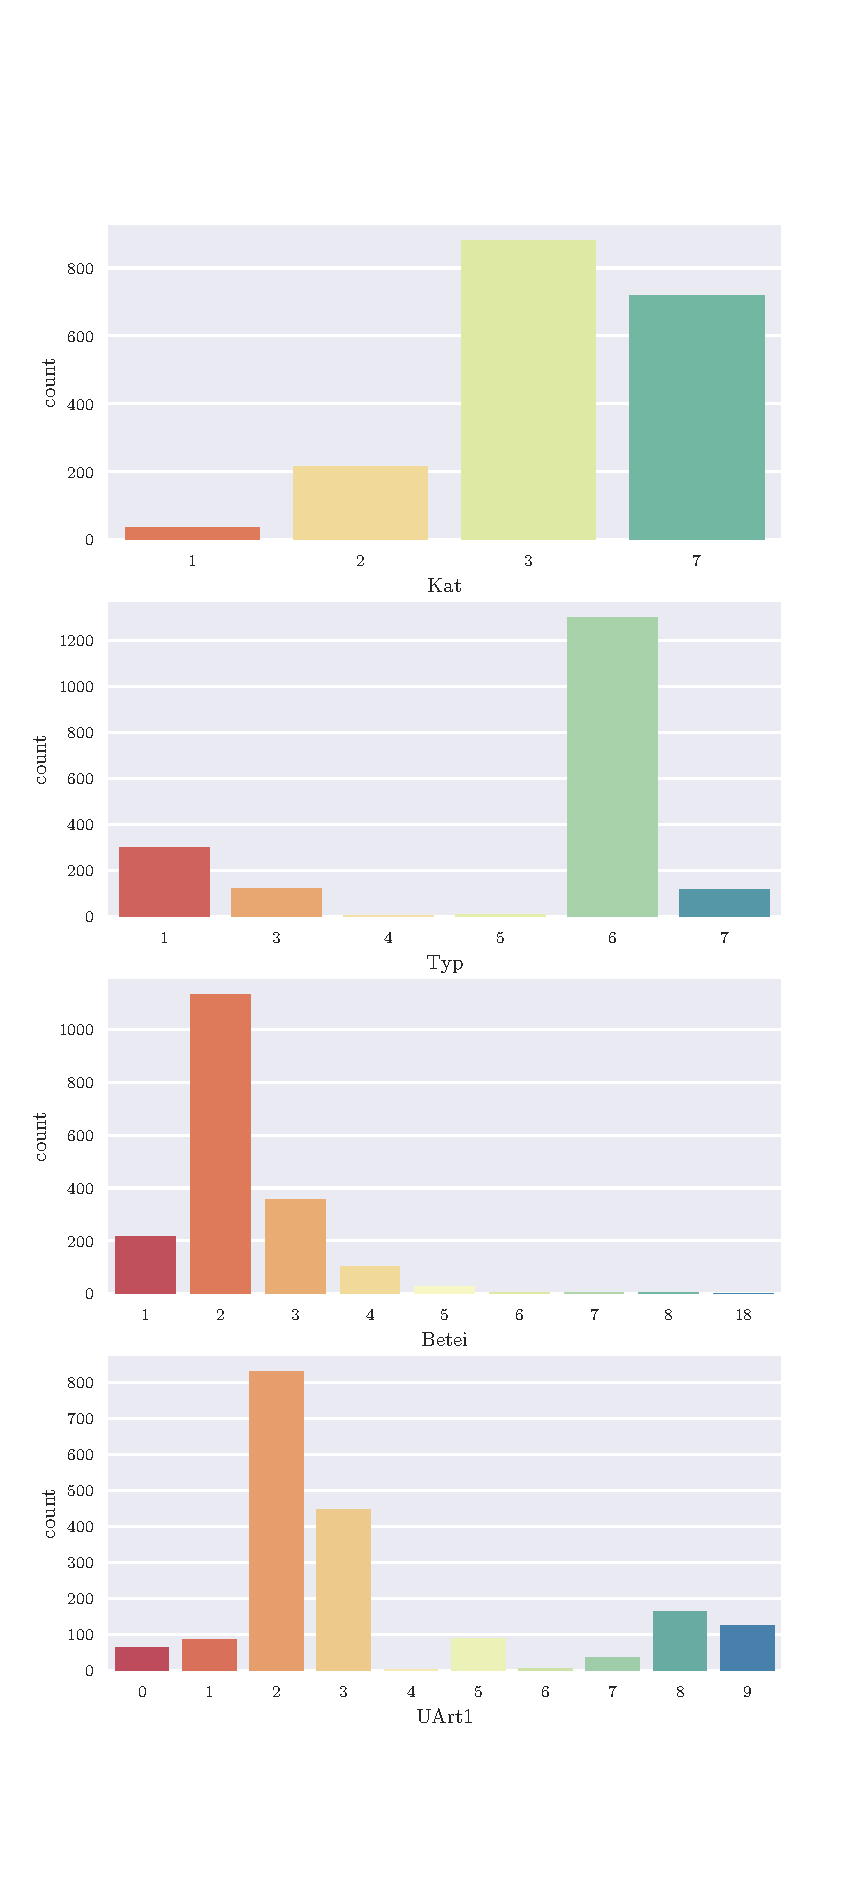
\includegraphics[scale=0.7]{CorrAnalysis/data/BAYSIS/02_matched/plots/baysis_matched_count_multiple01}
    %     \caption{Distribution of the accident category Kat, Typ, Betei and UArt}
    %     \label{img:baysis_matched_Kat}
    %     \label{img:baysis_matched_Typ}
    %     \label{img:baysis_matched_Betei}
    %     \label{img:baysis_matched_UArt}
    % \end{figure}

    % \begin{figure}[ht!]
    %     \centering
    %     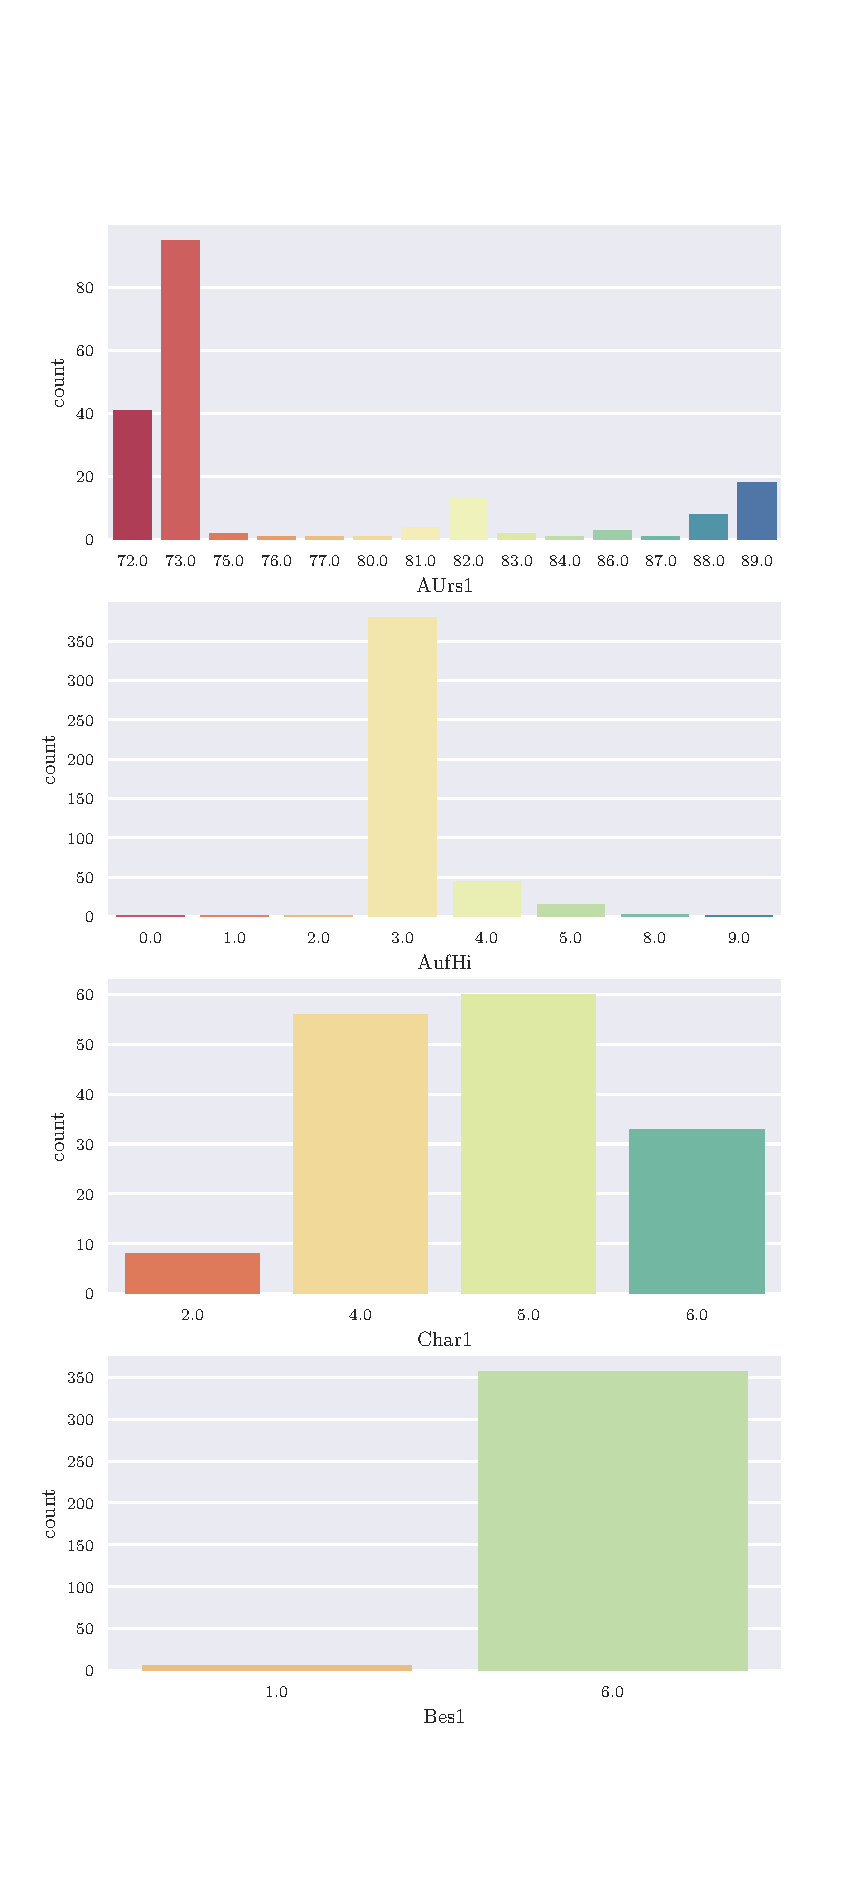
\includegraphics[scale=0.7]{CorrAnalysis/data/BAYSIS/02_matched/plots/baysis_matched_count_multiple02}
    %     \caption{Distribution of the accident category AUrs, AufHi, Char and Bes}
    %     \label{img:baysis_matched_AUrs}
    %     \label{img:baysis_matched_AufHi}
    %     \label{img:baysis_matched_Char}
    %     \label{img:baysis_matched_Bes}
    % \end{figure}

    % \begin{figure}[ht!]
    %     \centering
    %     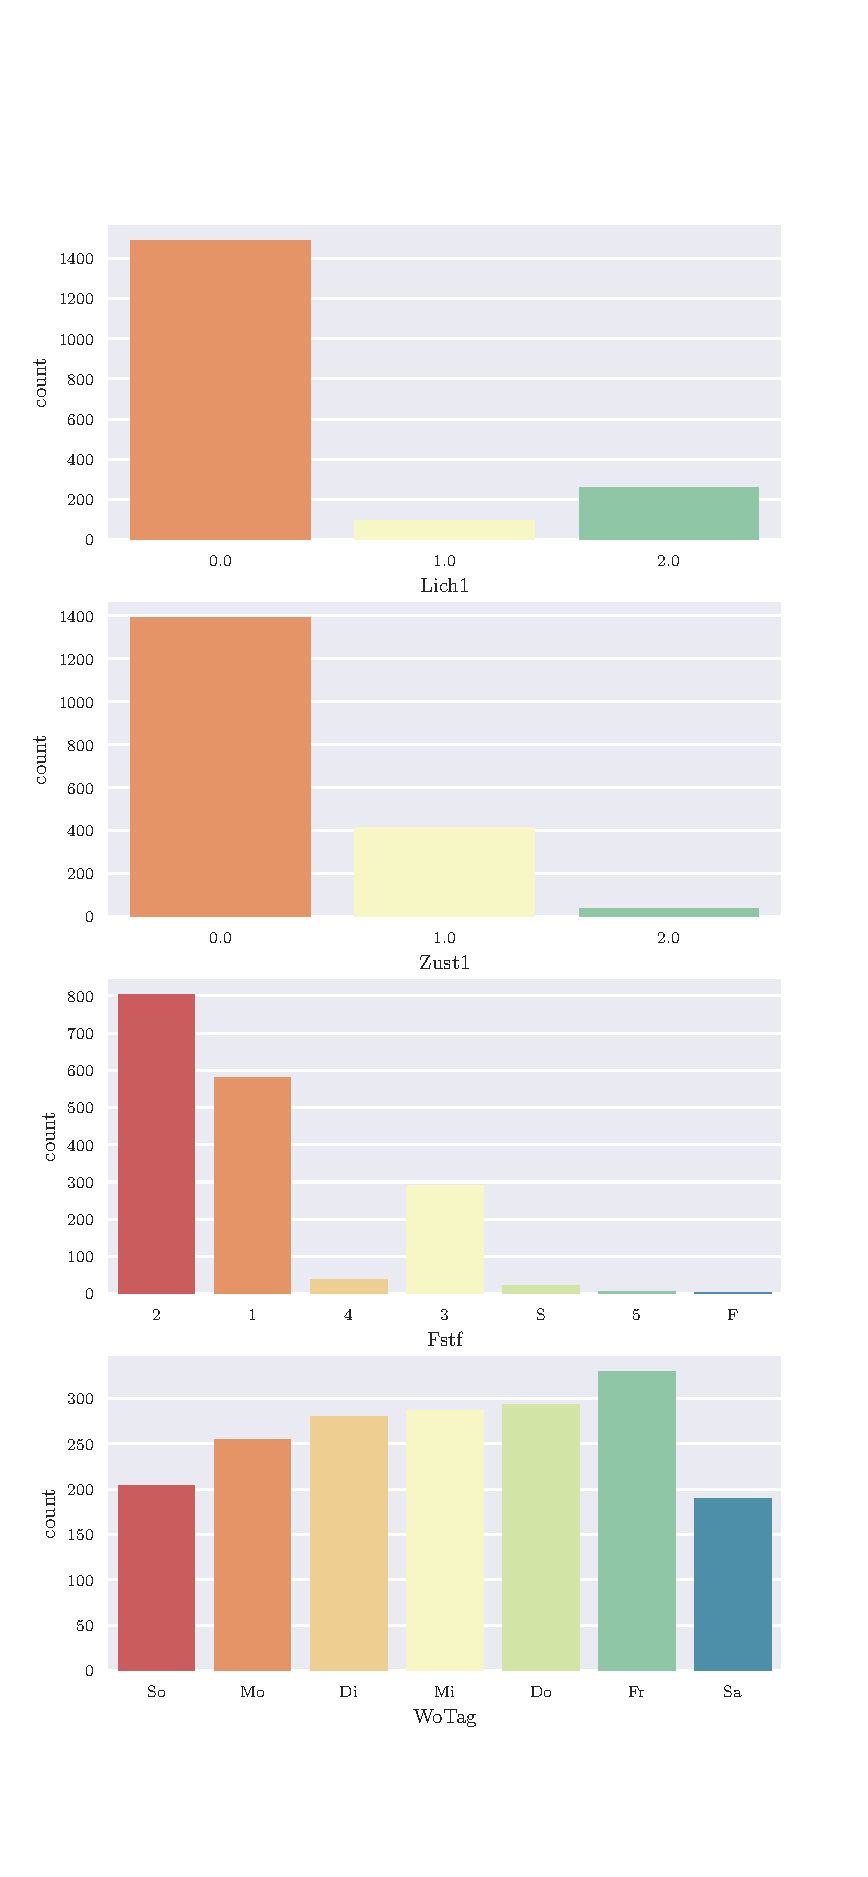
\includegraphics[scale=0.7]{CorrAnalysis/data/BAYSIS/02_matched/plots/baysis_matched_count_multiple03}
    %     \caption{Distribution of the accident category Lich, Zust, Fstf and WoTag}
    %     \label{img:baysis_matched_Lich}
    %     \label{img:baysis_matched_Zust}
    %     \label{img:baysis_matched_Fstf}
    %     \label{img:baysis_matched_WoTag}
    % \end{figure}
    
    % ------- BAYSIS Selected03 - Tables --------
    % \newgeometry{left=1cm,right=1cm,top=1cm}
    \begin{sidewaystable}
    	\tiny
    	\setlength{\tabcolsep}{2pt}
    	\centering
    	\begin{tabular}{lrrrrrrrrrrrrrrrrrrrrrrrrrrrrr}
\toprule
{} &  TMax &  TAvg &  SMax &  SAvg &  TDist &  SDist &   Cov &  TLCar &  TLHGV &  Str &  Kat &  Typ &  Betei &  UArt1 &  UArt2 &  AUrs1 &  AUrs2 &  AufHi &  Alkoh &  Char1 &  Char2 &  Lich1 &  Lich2 &  Zust1 &  Zust2 &  Fstf &  WoTag &  FeiTag &  Month \\
\midrule
TMax   &  1.00 &  0.81 &  0.49 &  0.50 &  -0.24 &  -0.05 & -0.12 &   0.05 &  -0.02 & 0.29 & 0.15 & 0.07 &   0.07 &   0.10 &   0.12 &   0.12 &   0.02 &   0.22 &   0.04 &   0.09 &   0.04 &   0.02 &   0.02 &   0.13 &   0.05 & -0.02 &   0.11 &   -0.00 &   0.19 \\
TAvg   &  0.81 &  1.00 &  0.19 &  0.45 &  -0.17 &  -0.03 &  0.24 &   0.01 &   0.01 & 0.22 & 0.13 & 0.12 &   0.08 &   0.16 &   0.07 &   0.07 &   0.01 &   0.33 &   0.04 &   0.05 &   0.03 &   0.10 &   0.08 &   0.09 &   0.04 & -0.02 &   0.15 &    0.00 &   0.15 \\
SMax   &  0.49 &  0.19 &  1.00 &  0.66 &  -0.21 &  -0.04 & -0.50 &   0.05 &  -0.10 & 0.35 & 0.18 & 0.10 &   0.07 &   0.17 &   0.09 &   0.10 &   0.02 &   0.11 &   0.03 &   0.07 &   0.04 &   0.08 &   0.06 &   0.09 &   0.04 &  0.05 &   0.15 &    0.05 &   0.21 \\
SAvg   &  0.50 &  0.45 &  0.66 &  1.00 &  -0.24 &  -0.11 &  0.09 &   0.01 &  -0.09 & 0.32 & 0.26 & 0.06 &   0.10 &   0.19 &   0.12 &   0.10 &   0.05 &   0.08 &   0.05 &   0.10 &   0.09 &   0.02 &   0.03 &   0.09 &   0.02 &  0.03 &   0.16 &    0.06 &   0.15 \\
TDist  & -0.24 & -0.17 & -0.21 & -0.24 &   1.00 &   0.08 &  0.03 &  -0.04 &   0.04 & 0.19 & 0.12 & 0.13 &  -0.09 &   0.24 &   0.15 &   0.20 &   0.02 &   0.07 &   0.02 &   0.09 &   0.08 &   0.01 &   0.03 &   0.10 &   0.05 &  0.01 &   0.15 &   -0.02 &   0.09 \\
SDist  & -0.05 & -0.03 & -0.04 & -0.11 &   0.08 &   1.00 &  0.00 &  -0.01 &   0.09 & 0.23 & 0.04 & 0.12 &  -0.03 &   0.12 &   0.10 &   0.17 &   0.02 &   0.07 &  -0.04 &   0.05 &   0.00 &   0.01 &   0.02 &   0.05 &   0.02 &  0.05 &   0.13 &    0.06 &   0.13 \\
Cov    & -0.12 &  0.24 & -0.50 &  0.09 &   0.03 &   0.00 &  1.00 &  -0.04 &   0.12 & 0.35 & 0.06 & 0.15 &   0.03 &   0.22 &   0.14 &   0.22 &   0.06 &   0.17 &  -0.01 &   0.08 &   0.05 &   0.15 &   0.14 &   0.14 &   0.02 & -0.01 &   0.18 &    0.01 &   0.23 \\
TLCar  &  0.05 &  0.01 &  0.05 &  0.01 &  -0.04 &  -0.01 & -0.04 &   1.00 &  -0.01 & 0.09 & 0.07 & 0.03 &   0.02 &   0.13 &   0.11 &   0.07 &   0.04 &   0.09 &  -0.02 &   0.12 &   0.01 &   0.09 &   0.09 &   0.07 &   0.04 & -0.01 &   0.14 &    0.03 &   0.11 \\
TLHGV  & -0.02 &  0.01 & -0.10 & -0.09 &   0.04 &   0.09 &  0.12 &  -0.01 &   1.00 & 0.24 & 0.06 & 0.11 &  -0.09 &   0.17 &   0.12 &   0.23 &   0.10 &   0.09 &  -0.05 &   0.11 &   0.05 &   0.06 &   0.05 &   0.12 &   0.00 & -0.01 &   0.20 &    0.03 &   0.18 \\
Str    &  0.29 &  0.22 &  0.35 &  0.32 &   0.19 &   0.23 &  0.35 &   0.09 &   0.24 & 1.00 & 0.15 & 0.23 &   0.15 &   0.20 &   0.14 &   0.24 &   0.14 &   0.17 &   0.12 &   0.23 &   0.41 &   0.23 &   0.17 &   0.25 &   0.16 &  0.20 &   0.18 &    0.13 &   0.19 \\
Kat    &  0.15 &  0.13 &  0.18 &  0.26 &   0.12 &   0.04 &  0.06 &   0.07 &   0.06 & 0.15 & 1.00 & 0.19 &   0.27 &   0.41 &   0.17 &   0.10 &   0.05 &   0.11 &   0.23 &   0.11 &   0.11 &   0.09 &   0.09 &   0.04 &   0.05 &  0.13 &   0.11 &    0.05 &   0.15 \\
Typ    &  0.07 &  0.12 &  0.10 &  0.06 &   0.13 &   0.12 &  0.15 &   0.03 &   0.11 & 0.23 & 0.19 & 1.00 &   0.36 &   0.52 &   0.13 &   0.30 &   0.09 &   0.32 &   0.07 &   0.10 &   0.25 &   0.13 &   0.24 &   0.20 &   0.13 &  0.24 &   0.14 &    0.10 &   0.18 \\
Betei  &  0.07 &  0.08 &  0.07 &  0.10 &  -0.09 &  -0.03 &  0.03 &   0.02 &  -0.09 & 0.15 & 0.27 & 0.36 &   1.00 &   0.33 &   0.20 &   0.20 &   0.03 &   0.37 &   0.06 &   0.11 &   0.26 &   0.13 &   0.11 &   0.17 &   0.07 &  0.17 &   0.12 &    0.07 &   0.17 \\
UArt1  &  0.10 &  0.16 &  0.17 &  0.19 &   0.24 &   0.12 &  0.22 &   0.13 &   0.17 & 0.20 & 0.41 & 0.52 &   0.33 &   1.00 &   0.33 &   0.32 &   0.15 &   0.51 &   0.13 &   0.13 &   0.23 &   0.14 &   0.15 &   0.19 &   0.12 &  0.21 &   0.14 &    0.11 &   0.17 \\
UArt2  &  0.12 &  0.07 &  0.09 &  0.12 &   0.15 &   0.10 &  0.14 &   0.11 &   0.12 & 0.14 & 0.17 & 0.13 &   0.20 &   0.33 &   1.00 &   0.12 &   0.01 &   0.42 &   0.03 &   0.08 &   0.13 &   0.09 &   0.07 &   0.11 &   0.03 &  0.12 &   0.13 &    0.06 &   0.16 \\
AUrs1  &  0.12 &  0.07 &  0.10 &  0.10 &   0.20 &   0.17 &  0.22 &   0.07 &   0.23 & 0.24 & 0.10 & 0.30 &   0.20 &   0.32 &   0.12 &   1.00 &   0.33 &   0.35 &   0.03 &   0.11 &   0.15 &   0.21 &   0.19 &   0.57 &   0.16 &  0.08 &   0.13 &    0.16 &   0.21 \\
AUrs2  &  0.02 &  0.01 &  0.02 &  0.05 &   0.02 &   0.02 &  0.06 &   0.04 &   0.10 & 0.14 & 0.05 & 0.09 &   0.03 &   0.15 &   0.01 &   0.33 &   1.00 &   0.02 &   0.01 &   0.01 &   0.01 &   0.16 &   0.08 &   0.33 &   0.01 &  0.06 &   0.11 &    0.01 &   0.18 \\
AufHi  &  0.22 &  0.33 &  0.11 &  0.08 &   0.07 &   0.07 &  0.17 &   0.09 &   0.09 & 0.17 & 0.11 & 0.32 &   0.37 &   0.51 &   0.42 &   0.35 &   0.02 &   1.00 &   0.05 &   0.12 &   0.30 &   0.07 &   0.08 &   0.16 &   0.04 &  0.18 &   0.14 &    0.18 &   0.16 \\
Alkoh  &  0.04 &  0.04 &  0.03 &  0.05 &   0.02 &  -0.04 & -0.01 &  -0.02 &  -0.05 & 0.12 & 0.23 & 0.07 &   0.06 &   0.13 &   0.03 &   0.03 &   0.01 &   0.05 &   1.00 &   0.03 &   0.07 &   0.08 &   0.01 &   0.06 &   0.09 &  0.09 &   0.07 &    0.05 &   0.13 \\
Char1  &  0.09 &  0.05 &  0.07 &  0.10 &   0.09 &   0.05 &  0.08 &   0.12 &   0.11 & 0.23 & 0.11 & 0.10 &   0.11 &   0.13 &   0.08 &   0.11 &   0.01 &   0.12 &   0.03 &   1.00 &   0.53 &   0.10 &   0.04 &   0.08 &   0.14 &  0.12 &   0.12 &    0.03 &   0.15 \\
Char2  &  0.04 &  0.03 &  0.04 &  0.09 &   0.08 &   0.00 &  0.05 &   0.01 &   0.05 & 0.41 & 0.11 & 0.25 &   0.26 &   0.23 &   0.13 &   0.15 &   0.01 &   0.30 &   0.07 &   0.53 &   1.00 &   0.08 &   0.06 &   0.13 &   0.09 &  0.21 &   0.07 &    0.05 &   0.15 \\
Lich1  &  0.02 &  0.10 &  0.08 &  0.02 &   0.01 &   0.01 &  0.15 &   0.09 &   0.06 & 0.23 & 0.09 & 0.13 &   0.13 &   0.14 &   0.09 &   0.21 &   0.16 &   0.07 &   0.08 &   0.10 &   0.08 &   1.00 &   0.71 &   0.19 &   0.10 &  0.11 &   0.22 &    0.05 &   0.34 \\
Lich2  &  0.02 &  0.08 &  0.06 &  0.03 &   0.03 &   0.02 &  0.14 &   0.09 &   0.05 & 0.17 & 0.09 & 0.24 &   0.11 &   0.15 &   0.07 &   0.19 &   0.08 &   0.08 &   0.01 &   0.04 &   0.06 &   0.71 &   1.00 &   0.19 &   0.03 &  0.12 &   0.19 &    0.03 &   0.33 \\
Zust1  &  0.13 &  0.09 &  0.09 &  0.09 &   0.10 &   0.05 &  0.14 &   0.07 &   0.12 & 0.25 & 0.04 & 0.20 &   0.17 &   0.19 &   0.11 &   0.57 &   0.33 &   0.16 &   0.06 &   0.08 &   0.13 &   0.19 &   0.19 &   1.00 &   0.19 &  0.08 &   0.17 &    0.10 &   0.30 \\
Zust2  &  0.05 &  0.04 &  0.04 &  0.02 &   0.05 &   0.02 &  0.02 &   0.04 &   0.00 & 0.16 & 0.05 & 0.13 &   0.07 &   0.12 &   0.03 &   0.16 &   0.01 &   0.04 &   0.09 &   0.14 &   0.09 &   0.10 &   0.03 &   0.19 &   1.00 &  0.10 &   0.08 &    0.07 &   0.25 \\
Fstf   & -0.02 & -0.02 &  0.05 &  0.03 &   0.01 &   0.05 & -0.01 &  -0.01 &  -0.01 & 0.20 & 0.13 & 0.24 &   0.17 &   0.21 &   0.12 &   0.08 &   0.06 &   0.18 &   0.09 &   0.12 &   0.21 &   0.11 &   0.12 &   0.08 &   0.10 &  1.00 &   0.11 &    0.13 &   0.14 \\
WoTag  &  0.11 &  0.15 &  0.15 &  0.16 &   0.15 &   0.13 &  0.18 &   0.14 &   0.20 & 0.18 & 0.11 & 0.14 &   0.12 &   0.14 &   0.13 &   0.13 &   0.11 &   0.14 &   0.07 &   0.12 &   0.07 &   0.22 &   0.19 &   0.17 &   0.08 &  0.11 &   1.00 &    0.16 &   0.18 \\
FeiTag & -0.00 &  0.00 &  0.05 &  0.06 &  -0.02 &   0.06 &  0.01 &   0.03 &   0.03 & 0.13 & 0.05 & 0.10 &   0.07 &   0.11 &   0.06 &   0.16 &   0.01 &   0.18 &   0.05 &   0.03 &   0.05 &   0.05 &   0.03 &   0.10 &   0.07 &  0.13 &   0.16 &    1.00 &   0.19 \\
Month  &  0.19 &  0.15 &  0.21 &  0.15 &   0.09 &   0.13 &  0.23 &   0.11 &   0.18 & 0.19 & 0.15 & 0.18 &   0.17 &   0.17 &   0.16 &   0.21 &   0.18 &   0.16 &   0.13 &   0.15 &   0.15 &   0.34 &   0.33 &   0.30 &   0.25 &  0.14 &   0.18 &    0.19 &   1.00 \\
\bottomrule
\end{tabular}

    	\caption{Correlation matrix for BAYSIS selected data (Jam Follower), calculated with Cramer's $V$, $\eta$, $\tau$, $r_{pq}$, $r$}
    	\label{table:appendix_correlation_matrix_selected_endJam_cramers}
    \end{sidewaystable}  
    \begin{sidewaystable}
    	\tiny
    	\setlength{\tabcolsep}{2pt}
    	\centering
    	\begin{tabular}{lrrrrrrrrrrrrrrrrrrrrrrrrrrrrr}
\toprule
{} &  TMax &  TAvg &  SMax &  SAvg &  TDist &  SDist &   Cov &  TLCar &  TLHGV &  Str &  Kat &  Typ &  Betei &  UArt1 &  UArt2 &  AUrs1 &  AUrs2 &  AufHi &  Alkoh &  Char1 &  Char2 &  Lich1 &  Lich2 &  Zust1 &  Zust2 &  Fstf &  WoTag &  FeiTag &  Month \\
\midrule
TMax   &  1.00 &  0.81 &  0.49 &  0.50 &  -0.24 &  -0.05 & -0.12 &   0.05 &  -0.02 & 0.29 & 0.15 & 0.07 &   0.07 &   0.10 &   0.12 &   0.12 &   0.02 &   0.22 &   0.04 &   0.09 &   0.04 &   0.02 &   0.02 &   0.13 &   0.05 & -0.02 &   0.11 &   -0.00 &   0.19 \\
TAvg   &  0.81 &  1.00 &  0.19 &  0.45 &  -0.17 &  -0.03 &  0.24 &   0.01 &   0.01 & 0.22 & 0.13 & 0.12 &   0.08 &   0.16 &   0.07 &   0.07 &   0.01 &   0.33 &   0.04 &   0.05 &   0.03 &   0.10 &   0.08 &   0.09 &   0.04 & -0.02 &   0.15 &    0.00 &   0.15 \\
SMax   &  0.49 &  0.19 &  1.00 &  0.66 &  -0.21 &  -0.04 & -0.50 &   0.05 &  -0.10 & 0.35 & 0.18 & 0.10 &   0.07 &   0.17 &   0.09 &   0.10 &   0.02 &   0.11 &   0.03 &   0.07 &   0.04 &   0.08 &   0.06 &   0.09 &   0.04 &  0.05 &   0.15 &    0.05 &   0.21 \\
SAvg   &  0.50 &  0.45 &  0.66 &  1.00 &  -0.24 &  -0.11 &  0.09 &   0.01 &  -0.09 & 0.32 & 0.26 & 0.06 &   0.10 &   0.19 &   0.12 &   0.10 &   0.05 &   0.08 &   0.05 &   0.10 &   0.09 &   0.02 &   0.03 &   0.09 &   0.02 &  0.03 &   0.16 &    0.06 &   0.15 \\
TDist  & -0.24 & -0.17 & -0.21 & -0.24 &   1.00 &   0.08 &  0.03 &  -0.04 &   0.04 & 0.19 & 0.12 & 0.13 &  -0.09 &   0.24 &   0.15 &   0.20 &   0.02 &   0.07 &   0.02 &   0.09 &   0.08 &   0.01 &   0.03 &   0.10 &   0.05 &  0.01 &   0.15 &   -0.02 &   0.09 \\
SDist  & -0.05 & -0.03 & -0.04 & -0.11 &   0.08 &   1.00 &  0.00 &  -0.01 &   0.09 & 0.23 & 0.04 & 0.12 &  -0.03 &   0.12 &   0.10 &   0.17 &   0.02 &   0.07 &  -0.04 &   0.05 &   0.00 &   0.01 &   0.02 &   0.05 &   0.02 &  0.05 &   0.13 &    0.06 &   0.13 \\
Cov    & -0.12 &  0.24 & -0.50 &  0.09 &   0.03 &   0.00 &  1.00 &  -0.04 &   0.12 & 0.35 & 0.06 & 0.15 &   0.03 &   0.22 &   0.14 &   0.22 &   0.06 &   0.17 &  -0.01 &   0.08 &   0.05 &   0.15 &   0.14 &   0.14 &   0.02 & -0.01 &   0.18 &    0.01 &   0.23 \\
TLCar  &  0.05 &  0.01 &  0.05 &  0.01 &  -0.04 &  -0.01 & -0.04 &   1.00 &  -0.01 & 0.09 & 0.07 & 0.03 &   0.02 &   0.13 &   0.11 &   0.07 &   0.04 &   0.09 &  -0.02 &   0.12 &   0.01 &   0.09 &   0.09 &   0.07 &   0.04 & -0.01 &   0.14 &    0.03 &   0.11 \\
TLHGV  & -0.02 &  0.01 & -0.10 & -0.09 &   0.04 &   0.09 &  0.12 &  -0.01 &   1.00 & 0.24 & 0.06 & 0.11 &  -0.09 &   0.17 &   0.12 &   0.23 &   0.10 &   0.09 &  -0.05 &   0.11 &   0.05 &   0.06 &   0.05 &   0.12 &   0.00 & -0.01 &   0.20 &    0.03 &   0.18 \\
Str    &  0.29 &  0.22 &  0.35 &  0.32 &   0.19 &   0.23 &  0.35 &   0.09 &   0.24 & 1.00 & 0.02 & 0.05 &   0.04 &   0.07 &   0.02 &   0.04 &   0.00 &   0.02 &   0.00 &   0.02 &   0.01 &   0.02 &   0.01 &   0.02 &   0.01 &  0.06 &   0.06 &    0.01 &   0.10 \\
Kat    &  0.15 &  0.13 &  0.18 &  0.26 &   0.12 &   0.04 &  0.06 &   0.07 &   0.06 & 0.05 & 1.00 & 0.08 &   0.14 &   0.31 &   0.04 &   0.02 &   0.00 &   0.02 &   0.01 &   0.02 &   0.01 &   0.01 &   0.01 &   0.00 &   0.00 &  0.03 &   0.02 &    0.00 &   0.04 \\
Typ    &  0.07 &  0.12 &  0.10 &  0.06 &   0.13 &   0.12 &  0.15 &   0.03 &   0.11 & 0.11 & 0.08 & 1.00 &   0.24 &   0.41 &   0.03 &   0.13 &   0.01 &   0.14 &   0.00 &   0.02 &   0.02 &   0.02 &   0.02 &   0.06 &   0.01 &  0.07 &   0.05 &    0.01 &   0.07 \\
Betei  &  0.07 &  0.08 &  0.07 &  0.10 &  -0.09 &  -0.03 &  0.03 &   0.02 &  -0.09 & 0.07 & 0.13 & 0.21 &   1.00 &   0.29 &   0.04 &   0.07 &   0.00 &   0.13 &   0.00 &   0.02 &   0.02 &   0.01 &   0.01 &   0.04 &   0.00 &  0.05 &   0.05 &    0.00 &   0.08 \\
UArt1  &  0.10 &  0.16 &  0.17 &  0.19 &   0.24 &   0.12 &  0.22 &   0.13 &   0.17 & 0.08 & 0.18 & 0.23 &   0.18 &   1.00 &   0.04 &   0.07 &   0.01 &   0.17 &   0.01 &   0.01 &   0.01 &   0.02 &   0.01 &   0.03 &   0.00 &  0.07 &   0.04 &    0.00 &   0.08 \\
UArt2  &  0.12 &  0.07 &  0.09 &  0.12 &   0.15 &   0.10 &  0.14 &   0.11 &   0.12 & 0.10 & 0.08 & 0.06 &   0.10 &   0.15 &   1.00 &   0.04 &   0.00 &   0.38 &   0.00 &   0.02 &   0.01 &   0.02 &   0.02 &   0.03 &   0.00 &  0.09 &   0.10 &    0.00 &   0.14 \\
AUrs1  &  0.12 &  0.07 &  0.10 &  0.10 &   0.20 &   0.17 &  0.22 &   0.07 &   0.23 & 0.18 & 0.04 & 0.30 &   0.19 &   0.29 &   0.05 &   1.00 &   0.05 &   0.24 &   0.00 &   0.03 &   0.01 &   0.07 &   0.07 &   0.41 &   0.01 &  0.07 &   0.12 &    0.02 &   0.24 \\
AUrs2  &  0.02 &  0.01 &  0.02 &  0.05 &   0.02 &   0.02 &  0.06 &   0.04 &   0.10 & 0.28 & 0.11 & 0.17 &   0.05 &   0.27 &   0.01 &   0.57 &   1.00 &   0.02 &   0.00 &   0.01 &   0.00 &   0.24 &   0.15 &   0.57 &   0.00 &  0.14 &   0.28 &    0.00 &   0.39 \\
AufHi  &  0.22 &  0.33 &  0.11 &  0.08 &   0.07 &   0.07 &  0.17 &   0.09 &   0.09 & 0.07 & 0.04 & 0.23 &   0.24 &   0.50 &   0.29 &   0.17 &   0.00 &   1.00 &   0.00 &   0.02 &   0.04 &   0.01 &   0.01 &   0.06 &   0.00 &  0.08 &   0.06 &    0.01 &   0.07 \\
Alkoh  &  0.04 &  0.04 &  0.03 &  0.05 &   0.02 &  -0.04 & -0.01 &  -0.02 &  -0.05 & 0.09 & 0.09 & 0.05 &   0.04 &   0.15 &   0.02 &   0.01 &   0.00 &   0.03 &   1.00 &   0.01 &   0.00 &   0.04 &   0.00 &   0.04 &   0.00 &  0.06 &   0.06 &    0.00 &   0.14 \\
Char1  &  0.09 &  0.05 &  0.07 &  0.10 &   0.09 &   0.05 &  0.08 &   0.12 &   0.11 & 0.16 & 0.05 & 0.05 &   0.06 &   0.07 &   0.03 &   0.04 &   0.00 &   0.04 &   0.00 &   1.00 &   0.17 &   0.03 &   0.01 &   0.03 &   0.01 &  0.07 &   0.09 &    0.00 &   0.14 \\
Char2  &  0.04 &  0.03 &  0.04 &  0.09 &   0.08 &   0.00 &  0.05 &   0.01 &   0.05 & 0.22 & 0.12 & 0.26 &   0.31 &   0.20 &   0.06 &   0.08 &   0.00 &   0.27 &   0.00 &   0.61 &   1.00 &   0.03 &   0.02 &   0.06 &   0.00 &  0.21 &   0.06 &    0.00 &   0.18 \\
Lich1  &  0.02 &  0.10 &  0.08 &  0.02 &   0.01 &   0.01 &  0.15 &   0.09 &   0.06 & 0.07 & 0.02 & 0.03 &   0.03 &   0.05 &   0.02 &   0.05 &   0.01 &   0.01 &   0.01 &   0.02 &   0.00 &   1.00 &   0.83 &   0.05 &   0.01 &  0.03 &   0.08 &    0.00 &   0.22 \\
Lich2  &  0.02 &  0.08 &  0.06 &  0.03 &   0.03 &   0.02 &  0.14 &   0.09 &   0.05 & 0.06 & 0.02 & 0.04 &   0.03 &   0.04 &   0.01 &   0.06 &   0.01 &   0.01 &   0.00 &   0.00 &   0.00 &   0.96 &   1.00 &   0.06 &   0.00 &  0.02 &   0.08 &    0.00 &   0.22 \\
Zust1  &  0.13 &  0.09 &  0.09 &  0.09 &   0.10 &   0.05 &  0.14 &   0.07 &   0.12 & 0.07 & 0.01 & 0.08 &   0.06 &   0.06 &   0.02 &   0.26 &   0.03 &   0.05 &   0.01 &   0.01 &   0.01 &   0.04 &   0.05 &   1.00 &   0.02 &  0.02 &   0.06 &    0.01 &   0.16 \\
Zust2  &  0.05 &  0.04 &  0.04 &  0.02 &   0.05 &   0.02 &  0.02 &   0.04 &   0.00 & 0.20 & 0.03 & 0.13 &   0.06 &   0.10 &   0.02 &   0.09 &   0.00 &   0.02 &   0.00 &   0.07 &   0.00 &   0.06 &   0.01 &   0.29 &   1.00 &  0.09 &   0.10 &    0.00 &   0.34 \\
Fstf   & -0.02 & -0.02 &  0.05 &  0.03 &   0.01 &   0.05 & -0.01 &  -0.01 &  -0.01 & 0.09 & 0.02 & 0.04 &   0.04 &   0.08 &   0.03 &   0.02 &   0.00 &   0.03 &   0.00 &   0.01 &   0.01 &   0.01 &   0.01 &   0.01 &   0.00 &  1.00 &   0.03 &    0.00 &   0.05 \\
WoTag  &  0.11 &  0.15 &  0.15 &  0.16 &   0.15 &   0.13 &  0.18 &   0.14 &   0.20 & 0.06 & 0.01 & 0.02 &   0.02 &   0.03 &   0.02 &   0.02 &   0.00 &   0.01 &   0.00 &   0.01 &   0.00 &   0.02 &   0.02 &   0.02 &   0.00 &  0.02 &   1.00 &    0.01 &   0.06 \\
FeiTag & -0.00 &  0.00 &  0.05 &  0.06 &  -0.02 &   0.06 &  0.01 &   0.03 &   0.03 & 0.10 & 0.02 & 0.05 &   0.03 &   0.06 &   0.02 &   0.07 &   0.00 &   0.05 &   0.00 &   0.01 &   0.00 &   0.02 &   0.00 &   0.03 &   0.00 &  0.04 &   0.14 &    1.00 &   0.19 \\
Month  &  0.19 &  0.15 &  0.21 &  0.15 &   0.09 &   0.13 &  0.23 &   0.11 &   0.18 & 0.08 & 0.02 & 0.03 &   0.03 &   0.05 &   0.02 &   0.04 &   0.00 &   0.02 &   0.00 &   0.02 &   0.01 &   0.05 &   0.04 &   0.04 &   0.01 &  0.02 &   0.05 &    0.01 &   1.00 \\
\bottomrule
\end{tabular}

    	\caption{Correlation matrix for BAYSIS selected data (Jam Follower), calculated with Theil's $U$, $\eta$, $\tau$, $r_{pq}$, $r$}
    	\label{table:appendix_correlation_matrix_selected_endJam_theils}
    \end{sidewaystable}
    \begin{sidewaystable}
    	\tiny
    	\setlength{\tabcolsep}{2pt}
    	\centering
    	\begin{tabular}{lrrrrrrrrrrrrrrrrrrrrrrrrrrrrr}
\toprule
{} &  TMax &  TAvg &  SMax &  SAvg &  TDist &  SDist &   Cov &  TLCar &  TLHGV &   Str &   Kat &   Typ &  Betei &  UArt1 &  UArt2 &  AUrs1 &  AUrs2 &  AufHi &  Alkoh &  Char1 &  Char2 &  Lich1 &  Lich2 &  Zust1 &  Zust2 &  Fstf &  WoTag &  FeiTag &  Month \\
\midrule
TMax   &   nan & 0.000 & 0.000 & 0.000 &  0.000 &  0.277 & 0.010 &  0.320 &  0.738 & 0.000 & 0.000 & 0.000 &  0.049 &  0.000 &  0.000 &  0.000 &  0.000 &  0.000 &  0.416 &  0.000 &  0.000 &  0.000 &  0.000 &  0.000 &  0.000 & 0.502 &  0.000 &   0.930 &  0.000 \\
TAvg   & 0.000 &   nan & 0.000 & 0.000 &  0.000 &  0.566 & 0.000 &  0.798 &  0.789 & 0.000 & 0.000 & 0.000 &  0.033 &  0.000 &  0.000 &  0.000 &  0.000 &  0.000 &  0.340 &  0.000 &  0.000 &  0.000 &  0.000 &  0.000 &  0.000 & 0.499 &  0.000 &   0.904 &  0.000 \\
SMax   & 0.000 & 0.000 &   nan & 0.000 &  0.000 &  0.378 & 0.000 &  0.314 &  0.038 & 0.000 & 0.000 & 0.000 &  0.057 &  0.000 &  0.000 &  0.000 &  0.000 &  0.000 &  0.514 &  0.000 &  0.000 &  0.000 &  0.000 &  0.000 &  0.000 & 0.126 &  0.000 &   0.189 &  0.000 \\
SAvg   & 0.000 & 0.000 & 0.000 &   nan &  0.000 &  0.021 & 0.046 &  0.810 &  0.061 & 0.000 & 0.000 & 0.000 &  0.005 &  0.000 &  0.000 &  0.000 &  0.000 &  0.000 &  0.321 &  0.000 &  0.000 &  0.000 &  0.000 &  0.000 &  0.000 & 0.342 &  0.000 &   0.125 &  0.000 \\
TDist  & 0.000 & 0.000 & 0.000 & 0.000 &    nan &  0.094 & 0.464 &  0.343 &  0.365 & 0.000 & 0.000 & 0.000 &  0.044 &  0.000 &  0.000 &  0.001 &  0.000 &  0.000 &  0.620 &  0.000 &  0.000 &  0.169 &  0.000 &  0.491 &  0.000 & 0.842 &  0.000 &   0.584 &  0.000 \\
SDist  & 0.277 & 0.566 & 0.378 & 0.021 &  0.094 &    nan & 0.971 &  0.870 &  0.043 & 0.000 & 0.000 & 0.000 &  0.517 &  0.000 &  0.000 &  0.000 &  0.000 &  0.000 &  0.392 &  0.000 &  0.000 &  0.001 &  0.000 &  0.191 &  0.000 & 0.226 &  0.000 &   0.195 &  0.000 \\
Cov    & 0.010 & 0.000 & 0.000 & 0.046 &  0.464 &  0.971 &   nan &  0.337 &  0.008 & 0.000 & 0.000 & 0.000 &  0.453 &  0.000 &  0.000 &  0.000 &  0.000 &  0.000 &  0.769 &  0.000 &  0.000 &  0.000 &  0.000 &  0.000 &  0.000 & 0.840 &  0.000 &   0.800 &  0.000 \\
TLCar  & 0.320 & 0.798 & 0.314 & 0.810 &  0.343 &  0.870 & 0.337 &    nan &  0.803 & 0.000 & 0.000 & 0.000 &  0.639 &  0.000 &  0.000 &  0.000 &  0.000 &  0.000 &  0.604 &  0.000 &  0.000 &  0.000 &  0.000 &  0.000 &  0.000 & 0.822 &  0.000 &   0.360 &  0.000 \\
TLHGV  & 0.738 & 0.789 & 0.038 & 0.061 &  0.365 &  0.043 & 0.008 &  0.803 &    nan & 0.000 & 0.000 & 0.000 &  0.017 &  0.000 &  0.000 &  0.000 &  0.000 &  0.000 &  0.300 &  0.000 &  0.000 &  0.000 &  0.000 &  0.000 &  0.000 & 0.886 &  0.000 &   0.419 &  0.000 \\
Str    & 0.000 & 0.000 & 0.000 & 0.000 &  0.000 &  0.000 & 0.000 &  0.000 &  0.000 &   nan & 0.507 & 0.000 &  0.696 &  0.000 &  0.772 &  0.000 &  0.616 &  0.128 &  0.817 &  0.000 &  0.000 &  0.001 &  0.207 &  0.000 &  0.390 & 0.000 &  0.037 &   0.738 &  0.001 \\
Kat    & 0.000 & 0.000 & 0.000 & 0.000 &  0.000 &  0.000 & 0.000 &  0.000 &  0.000 & 0.507 &   nan & 0.000 &  0.000 &  0.000 &  0.001 &  0.729 &  0.867 &  0.043 &  0.000 &  0.068 &  0.111 &  0.287 &  0.252 &  0.980 &  0.793 & 0.134 &  0.631 &   0.727 &  0.593 \\
Typ    & 0.000 & 0.000 & 0.000 & 0.000 &  0.000 &  0.000 & 0.000 &  0.000 &  0.000 & 0.000 & 0.000 &   nan &  0.000 &  0.000 &  0.194 &  0.000 &  0.455 &  0.000 &  0.731 &  0.365 &  0.000 &  0.068 &  0.000 &  0.000 &  0.099 & 0.000 &  0.107 &   0.377 &  0.067 \\
Betei  & 0.049 & 0.033 & 0.057 & 0.005 &  0.044 &  0.517 & 0.453 &  0.639 &  0.017 & 0.696 & 0.000 & 0.000 &    nan &  0.000 &  0.000 &  0.000 &  1.000 &  0.000 &  0.975 &  0.770 &  0.000 &  0.290 &  0.588 &  0.007 &  0.940 & 0.001 &  0.453 &   0.932 &  0.055 \\
UArt1  & 0.000 & 0.000 & 0.000 & 0.000 &  0.000 &  0.000 & 0.000 &  0.000 &  0.000 & 0.000 & 0.000 & 0.000 &  0.000 &    nan &  0.000 &  0.000 &  0.164 &  0.000 &  0.465 &  0.544 &  0.002 &  0.339 &  0.188 &  0.002 &  0.533 & 0.000 &  0.344 &   0.677 &  0.045 \\
UArt2  & 0.000 & 0.000 & 0.000 & 0.000 &  0.000 &  0.000 & 0.000 &  0.000 &  0.000 & 0.772 & 0.001 & 0.194 &  0.000 &  0.000 &    nan &  0.298 &  1.000 &  0.000 &  0.997 &  0.961 &  0.215 &  0.802 &  0.957 &  0.606 &  0.999 & 0.379 &  0.306 &   0.963 &  0.380 \\
AUrs1  & 0.000 & 0.000 & 0.000 & 0.000 &  0.001 &  0.000 & 0.000 &  0.000 &  0.000 & 0.000 & 0.729 & 0.000 &  0.000 &  0.000 &  0.298 &    nan &  0.000 &  0.000 &  0.998 &  0.525 &  0.107 &  0.000 &  0.001 &  0.000 &  0.076 & 0.988 &  0.312 &   0.055 &  0.000 \\
AUrs2  & 0.000 & 0.000 & 0.000 & 0.000 &  0.000 &  0.000 & 0.000 &  0.000 &  0.000 & 0.616 & 0.867 & 0.455 &  1.000 &  0.164 &  1.000 &  0.000 &    nan &  0.999 &  0.987 &  1.000 &  0.987 &  0.000 &  0.184 &  0.000 &  0.991 & 0.990 &  0.597 &   0.978 &  0.094 \\
AufHi  & 0.000 & 0.000 & 0.000 & 0.000 &  0.000 &  0.000 & 0.000 &  0.000 &  0.000 & 0.128 & 0.043 & 0.000 &  0.000 &  0.000 &  0.000 &  0.000 &  0.999 &    nan &  0.777 &  0.010 &  0.000 &  0.524 &  0.501 &  0.000 &  0.874 & 0.001 &  0.142 &   0.002 &  0.324 \\
Alkoh  & 0.416 & 0.340 & 0.514 & 0.321 &  0.620 &  0.392 & 0.769 &  0.604 &  0.300 & 0.817 & 0.000 & 0.731 &  0.975 &  0.465 &  0.997 &  0.998 &  0.987 &  0.777 &    nan &  0.954 &  0.124 &  0.224 &  0.973 &  0.653 &  0.046 & 0.712 &  0.940 &   0.294 &  0.702 \\
Char1  & 0.000 & 0.000 & 0.000 & 0.000 &  0.000 &  0.000 & 0.000 &  0.000 &  0.000 & 0.000 & 0.068 & 0.365 &  0.770 &  0.544 &  0.961 &  0.525 &  1.000 &  0.010 &  0.954 &    nan &  0.000 &  0.160 &  0.966 &  0.436 &  0.029 & 0.410 &  0.581 &   0.906 &  0.495 \\
Char2  & 0.000 & 0.000 & 0.000 & 0.000 &  0.000 &  0.000 & 0.000 &  0.000 &  0.000 & 0.000 & 0.111 & 0.000 &  0.000 &  0.002 &  0.215 &  0.107 &  0.987 &  0.000 &  0.124 &  0.000 &    nan &  0.245 &  0.400 &  0.044 &  0.046 & 0.003 &  0.920 &   0.294 &  0.464 \\
Lich1  & 0.000 & 0.000 & 0.000 & 0.000 &  0.169 &  0.001 & 0.000 &  0.000 &  0.000 & 0.001 & 0.287 & 0.068 &  0.290 &  0.339 &  0.802 &  0.000 &  0.000 &  0.524 &  0.224 &  0.160 &  0.245 &    nan &  0.000 &  0.000 &  0.091 & 0.563 &  0.000 &   0.518 &  0.000 \\
Lich2  & 0.000 & 0.000 & 0.000 & 0.000 &  0.000 &  0.000 & 0.000 &  0.000 &  0.000 & 0.207 & 0.252 & 0.000 &  0.588 &  0.188 &  0.957 &  0.001 &  0.184 &  0.501 &  0.973 &  0.966 &  0.400 &  0.000 &    nan &  0.000 &  0.820 & 0.382 &  0.001 &   0.853 &  0.000 \\
Zust1  & 0.000 & 0.000 & 0.000 & 0.000 &  0.491 &  0.191 & 0.000 &  0.000 &  0.000 & 0.000 & 0.980 & 0.000 &  0.007 &  0.002 &  0.606 &  0.000 &  0.000 &  0.000 &  0.653 &  0.436 &  0.044 &  0.000 &  0.000 &    nan &  0.001 & 0.967 &  0.007 &   0.207 &  0.000 \\
Zust2  & 0.000 & 0.000 & 0.000 & 0.000 &  0.000 &  0.000 & 0.000 &  0.000 &  0.000 & 0.390 & 0.793 & 0.099 &  0.940 &  0.533 &  0.999 &  0.076 &  0.991 &  0.874 &  0.046 &  0.029 &  0.046 &  0.091 &  0.820 &  0.001 &    nan & 0.592 &  0.852 &   0.152 &  0.002 \\
Fstf   & 0.502 & 0.499 & 0.126 & 0.342 &  0.842 &  0.226 & 0.840 &  0.822 &  0.886 & 0.000 & 0.134 & 0.000 &  0.001 &  0.000 &  0.379 &  0.988 &  0.990 &  0.001 &  0.712 &  0.410 &  0.003 &  0.563 &  0.382 &  0.967 &  0.592 &   nan &  0.850 &   0.281 &  0.819 \\
WoTag  & 0.000 & 0.000 & 0.000 & 0.000 &  0.000 &  0.000 & 0.000 &  0.000 &  0.000 & 0.037 & 0.631 & 0.107 &  0.453 &  0.344 &  0.306 &  0.312 &  0.597 &  0.142 &  0.940 &  0.581 &  0.920 &  0.000 &  0.001 &  0.007 &  0.852 & 0.850 &    nan &   0.100 &  0.011 \\
FeiTag & 0.930 & 0.904 & 0.189 & 0.125 &  0.584 &  0.195 & 0.800 &  0.360 &  0.419 & 0.738 & 0.727 & 0.377 &  0.932 &  0.677 &  0.963 &  0.055 &  0.978 &  0.002 &  0.294 &  0.906 &  0.294 &  0.518 &  0.853 &  0.207 &  0.152 & 0.281 &  0.100 &     nan &  0.092 \\
Month  & 0.000 & 0.000 & 0.000 & 0.000 &  0.000 &  0.000 & 0.000 &  0.000 &  0.000 & 0.001 & 0.593 & 0.067 &  0.055 &  0.045 &  0.380 &  0.000 &  0.094 &  0.324 &  0.702 &  0.495 &  0.464 &  0.000 &  0.000 &  0.000 &  0.002 & 0.819 &  0.011 &   0.092 &    nan \\
\bottomrule
\end{tabular}

    	\caption{Significancy matrix for BAYSIS selected data (Jam Follower)}
    	\label{table:appendix_significancy_matrix_selected_endJam}
    \end{sidewaystable}
    \begin{sidewaystable}
    	\tiny
    	\setlength{\tabcolsep}{2pt}
    	\centering
    	\begin{tabular}{llllllllllllllllllllllllllllll}
\toprule
{} &      TMax &      TAvg &      SMax &      SAvg &     TDist &     SDist &       Cov &     TLCar &     TLHGV &     Str &     Kat &     Typ &   Betei &   UArt1 &   UArt2 &   AUrs1 &   AUrs2 &   AufHi &     Alkoh &   Char1 &   Char2 &   Lich1 &   Lich2 &   Zust1 &   Zust2 &    Fstf &   WoTag &  FeiTag &   Month \\
\midrule
TMax   &       NaN &       $r$ &       $r$ &       $r$ &       $r$ &       $r$ &       $r$ &       $r$ &       $r$ &  $\eta$ &  $\eta$ &  $\eta$ &  $\tau$ &  $\eta$ &  $\eta$ &  $\eta$ &  $\eta$ &  $\eta$ &  $r_{pq}$ &  $\eta$ &  $\eta$ &  $\eta$ &  $\eta$ &  $\eta$ &  $\eta$ &  $\tau$ &  $\eta$ &  $\tau$ &  $\eta$ \\
TAvg   &       $r$ &       NaN &       $r$ &       $r$ &       $r$ &       $r$ &       $r$ &       $r$ &       $r$ &  $\eta$ &  $\eta$ &  $\eta$ &  $\tau$ &  $\eta$ &  $\eta$ &  $\eta$ &  $\eta$ &  $\eta$ &  $r_{pq}$ &  $\eta$ &  $\eta$ &  $\eta$ &  $\eta$ &  $\eta$ &  $\eta$ &  $\tau$ &  $\eta$ &  $\tau$ &  $\eta$ \\
SMax   &       $r$ &       $r$ &       NaN &       $r$ &       $r$ &       $r$ &       $r$ &       $r$ &       $r$ &  $\eta$ &  $\eta$ &  $\eta$ &  $\tau$ &  $\eta$ &  $\eta$ &  $\eta$ &  $\eta$ &  $\eta$ &  $r_{pq}$ &  $\eta$ &  $\eta$ &  $\eta$ &  $\eta$ &  $\eta$ &  $\eta$ &  $\tau$ &  $\eta$ &  $\tau$ &  $\eta$ \\
SAvg   &       $r$ &       $r$ &       $r$ &       NaN &       $r$ &       $r$ &       $r$ &       $r$ &       $r$ &  $\eta$ &  $\eta$ &  $\eta$ &  $\tau$ &  $\eta$ &  $\eta$ &  $\eta$ &  $\eta$ &  $\eta$ &  $r_{pq}$ &  $\eta$ &  $\eta$ &  $\eta$ &  $\eta$ &  $\eta$ &  $\eta$ &  $\tau$ &  $\eta$ &  $\tau$ &  $\eta$ \\
TDist  &       $r$ &       $r$ &       $r$ &       $r$ &       NaN &       $r$ &       $r$ &       $r$ &       $r$ &  $\eta$ &  $\eta$ &  $\eta$ &  $\tau$ &  $\eta$ &  $\eta$ &  $\eta$ &  $\eta$ &  $\eta$ &  $r_{pq}$ &  $\eta$ &  $\eta$ &  $\eta$ &  $\eta$ &  $\eta$ &  $\eta$ &  $\tau$ &  $\eta$ &  $\tau$ &  $\eta$ \\
SDist  &       $r$ &       $r$ &       $r$ &       $r$ &       $r$ &       NaN &       $r$ &       $r$ &       $r$ &  $\eta$ &  $\eta$ &  $\eta$ &  $\tau$ &  $\eta$ &  $\eta$ &  $\eta$ &  $\eta$ &  $\eta$ &  $r_{pq}$ &  $\eta$ &  $\eta$ &  $\eta$ &  $\eta$ &  $\eta$ &  $\eta$ &  $\tau$ &  $\eta$ &  $\tau$ &  $\eta$ \\
Cov    &       $r$ &       $r$ &       $r$ &       $r$ &       $r$ &       $r$ &       NaN &       $r$ &       $r$ &  $\eta$ &  $\eta$ &  $\eta$ &  $\tau$ &  $\eta$ &  $\eta$ &  $\eta$ &  $\eta$ &  $\eta$ &  $r_{pq}$ &  $\eta$ &  $\eta$ &  $\eta$ &  $\eta$ &  $\eta$ &  $\eta$ &  $\tau$ &  $\eta$ &  $\tau$ &  $\eta$ \\
TLCar  &       $r$ &       $r$ &       $r$ &       $r$ &       $r$ &       $r$ &       $r$ &       NaN &       $r$ &  $\eta$ &  $\eta$ &  $\eta$ &  $\tau$ &  $\eta$ &  $\eta$ &  $\eta$ &  $\eta$ &  $\eta$ &  $r_{pq}$ &  $\eta$ &  $\eta$ &  $\eta$ &  $\eta$ &  $\eta$ &  $\eta$ &  $\tau$ &  $\eta$ &  $\tau$ &  $\eta$ \\
TLHGV  &       $r$ &       $r$ &       $r$ &       $r$ &       $r$ &       $r$ &       $r$ &       $r$ &       NaN &  $\eta$ &  $\eta$ &  $\eta$ &  $\tau$ &  $\eta$ &  $\eta$ &  $\eta$ &  $\eta$ &  $\eta$ &  $r_{pq}$ &  $\eta$ &  $\eta$ &  $\eta$ &  $\eta$ &  $\eta$ &  $\eta$ &  $\tau$ &  $\eta$ &  $\tau$ &  $\eta$ \\
Str    &    $\eta$ &    $\eta$ &    $\eta$ &    $\eta$ &    $\eta$ &    $\eta$ &    $\eta$ &    $\eta$ &    $\eta$ &     NaN &     $V$ &     $V$ &     $V$ &     $V$ &     $V$ &     $V$ &     $V$ &     $V$ &       $V$ &     $V$ &     $V$ &     $V$ &     $V$ &     $V$ &     $V$ &     $V$ &     $V$ &     $V$ &     $V$ \\
Kat    &    $\eta$ &    $\eta$ &    $\eta$ &    $\eta$ &    $\eta$ &    $\eta$ &    $\eta$ &    $\eta$ &    $\eta$ &     $V$ &     NaN &     $V$ &     $V$ &     $V$ &     $V$ &     $V$ &     $V$ &     $V$ &       $V$ &     $V$ &     $V$ &     $V$ &     $V$ &     $V$ &     $V$ &     $V$ &     $V$ &     $V$ &     $V$ \\
Typ    &    $\eta$ &    $\eta$ &    $\eta$ &    $\eta$ &    $\eta$ &    $\eta$ &    $\eta$ &    $\eta$ &    $\eta$ &     $V$ &     $V$ &     NaN &     $V$ &     $V$ &     $V$ &     $V$ &     $V$ &     $V$ &       $V$ &     $V$ &     $V$ &     $V$ &     $V$ &     $V$ &     $V$ &     $V$ &     $V$ &     $V$ &     $V$ \\
Betei  &    $\tau$ &    $\tau$ &    $\tau$ &    $\tau$ &    $\tau$ &    $\tau$ &    $\tau$ &    $\tau$ &    $\tau$ &     $V$ &     $V$ &     $V$ &     NaN &     $V$ &     $V$ &     $V$ &     $V$ &     $V$ &       $V$ &     $V$ &     $V$ &     $V$ &     $V$ &     $V$ &     $V$ &     $V$ &     $V$ &     $V$ &     $V$ \\
UArt1  &    $\eta$ &    $\eta$ &    $\eta$ &    $\eta$ &    $\eta$ &    $\eta$ &    $\eta$ &    $\eta$ &    $\eta$ &     $V$ &     $V$ &     $V$ &     $V$ &     NaN &     $V$ &     $V$ &     $V$ &     $V$ &       $V$ &     $V$ &     $V$ &     $V$ &     $V$ &     $V$ &     $V$ &     $V$ &     $V$ &     $V$ &     $V$ \\
UArt2  &    $\eta$ &    $\eta$ &    $\eta$ &    $\eta$ &    $\eta$ &    $\eta$ &    $\eta$ &    $\eta$ &    $\eta$ &     $V$ &     $V$ &     $V$ &     $V$ &     $V$ &     NaN &     $V$ &     $V$ &     $V$ &       $V$ &     $V$ &     $V$ &     $V$ &     $V$ &     $V$ &     $V$ &     $V$ &     $V$ &     $V$ &     $V$ \\
AUrs1  &    $\eta$ &    $\eta$ &    $\eta$ &    $\eta$ &    $\eta$ &    $\eta$ &    $\eta$ &    $\eta$ &    $\eta$ &     $V$ &     $V$ &     $V$ &     $V$ &     $V$ &     $V$ &     NaN &     $V$ &     $V$ &       $V$ &     $V$ &     $V$ &     $V$ &     $V$ &     $V$ &     $V$ &     $V$ &     $V$ &     $V$ &     $V$ \\
AUrs2  &    $\eta$ &    $\eta$ &    $\eta$ &    $\eta$ &    $\eta$ &    $\eta$ &    $\eta$ &    $\eta$ &    $\eta$ &     $V$ &     $V$ &     $V$ &     $V$ &     $V$ &     $V$ &     $V$ &     NaN &     $V$ &       $V$ &     $V$ &     $V$ &     $V$ &     $V$ &     $V$ &     $V$ &     $V$ &     $V$ &     $V$ &     $V$ \\
AufHi  &    $\eta$ &    $\eta$ &    $\eta$ &    $\eta$ &    $\eta$ &    $\eta$ &    $\eta$ &    $\eta$ &    $\eta$ &     $V$ &     $V$ &     $V$ &     $V$ &     $V$ &     $V$ &     $V$ &     $V$ &     NaN &       $V$ &     $V$ &     $V$ &     $V$ &     $V$ &     $V$ &     $V$ &     $V$ &     $V$ &     $V$ &     $V$ \\
Alkoh  &  $r_{pq}$ &  $r_{pq}$ &  $r_{pq}$ &  $r_{pq}$ &  $r_{pq}$ &  $r_{pq}$ &  $r_{pq}$ &  $r_{pq}$ &  $r_{pq}$ &     $V$ &     $V$ &     $V$ &     $V$ &     $V$ &     $V$ &     $V$ &     $V$ &     $V$ &       NaN &     $V$ &     $V$ &     $V$ &     $V$ &     $V$ &     $V$ &     $V$ &     $V$ &     $V$ &     $V$ \\
Char1  &    $\eta$ &    $\eta$ &    $\eta$ &    $\eta$ &    $\eta$ &    $\eta$ &    $\eta$ &    $\eta$ &    $\eta$ &     $V$ &     $V$ &     $V$ &     $V$ &     $V$ &     $V$ &     $V$ &     $V$ &     $V$ &       $V$ &     NaN &     $V$ &     $V$ &     $V$ &     $V$ &     $V$ &     $V$ &     $V$ &     $V$ &     $V$ \\
Char2  &    $\eta$ &    $\eta$ &    $\eta$ &    $\eta$ &    $\eta$ &    $\eta$ &    $\eta$ &    $\eta$ &    $\eta$ &     $V$ &     $V$ &     $V$ &     $V$ &     $V$ &     $V$ &     $V$ &     $V$ &     $V$ &       $V$ &     $V$ &     NaN &     $V$ &     $V$ &     $V$ &     $V$ &     $V$ &     $V$ &     $V$ &     $V$ \\
Lich1  &    $\eta$ &    $\eta$ &    $\eta$ &    $\eta$ &    $\eta$ &    $\eta$ &    $\eta$ &    $\eta$ &    $\eta$ &     $V$ &     $V$ &     $V$ &     $V$ &     $V$ &     $V$ &     $V$ &     $V$ &     $V$ &       $V$ &     $V$ &     $V$ &     NaN &     $V$ &     $V$ &     $V$ &     $V$ &     $V$ &     $V$ &     $V$ \\
Lich2  &    $\eta$ &    $\eta$ &    $\eta$ &    $\eta$ &    $\eta$ &    $\eta$ &    $\eta$ &    $\eta$ &    $\eta$ &     $V$ &     $V$ &     $V$ &     $V$ &     $V$ &     $V$ &     $V$ &     $V$ &     $V$ &       $V$ &     $V$ &     $V$ &     $V$ &     NaN &     $V$ &     $V$ &     $V$ &     $V$ &     $V$ &     $V$ \\
Zust1  &    $\eta$ &    $\eta$ &    $\eta$ &    $\eta$ &    $\eta$ &    $\eta$ &    $\eta$ &    $\eta$ &    $\eta$ &     $V$ &     $V$ &     $V$ &     $V$ &     $V$ &     $V$ &     $V$ &     $V$ &     $V$ &       $V$ &     $V$ &     $V$ &     $V$ &     $V$ &     NaN &     $V$ &     $V$ &     $V$ &     $V$ &     $V$ \\
Zust2  &    $\eta$ &    $\eta$ &    $\eta$ &    $\eta$ &    $\eta$ &    $\eta$ &    $\eta$ &    $\eta$ &    $\eta$ &     $V$ &     $V$ &     $V$ &     $V$ &     $V$ &     $V$ &     $V$ &     $V$ &     $V$ &       $V$ &     $V$ &     $V$ &     $V$ &     $V$ &     $V$ &     NaN &     $V$ &     $V$ &     $V$ &     $V$ \\
Fstf   &    $\tau$ &    $\tau$ &    $\tau$ &    $\tau$ &    $\tau$ &    $\tau$ &    $\tau$ &    $\tau$ &    $\tau$ &     $V$ &     $V$ &     $V$ &     $V$ &     $V$ &     $V$ &     $V$ &     $V$ &     $V$ &       $V$ &     $V$ &     $V$ &     $V$ &     $V$ &     $V$ &     $V$ &     NaN &     $V$ &     $V$ &     $V$ \\
WoTag  &    $\eta$ &    $\eta$ &    $\eta$ &    $\eta$ &    $\eta$ &    $\eta$ &    $\eta$ &    $\eta$ &    $\eta$ &     $V$ &     $V$ &     $V$ &     $V$ &     $V$ &     $V$ &     $V$ &     $V$ &     $V$ &       $V$ &     $V$ &     $V$ &     $V$ &     $V$ &     $V$ &     $V$ &     $V$ &     NaN &     $V$ &     $V$ \\
FeiTag &    $\tau$ &    $\tau$ &    $\tau$ &    $\tau$ &    $\tau$ &    $\tau$ &    $\tau$ &    $\tau$ &    $\tau$ &     $V$ &     $V$ &     $V$ &     $V$ &     $V$ &     $V$ &     $V$ &     $V$ &     $V$ &       $V$ &     $V$ &     $V$ &     $V$ &     $V$ &     $V$ &     $V$ &     $V$ &     $V$ &     NaN &     $V$ \\
Month  &    $\eta$ &    $\eta$ &    $\eta$ &    $\eta$ &    $\eta$ &    $\eta$ &    $\eta$ &    $\eta$ &    $\eta$ &     $V$ &     $V$ &     $V$ &     $V$ &     $V$ &     $V$ &     $V$ &     $V$ &     $V$ &       $V$ &     $V$ &     $V$ &     $V$ &     $V$ &     $V$ &     $V$ &     $V$ &     $V$ &     $V$ &     NaN \\
\bottomrule
\end{tabular}

    	\caption{Coefficient matrix for BAYSIS selected data (Jam Follower)}
    	\label{table:appendix_coefficient_matrix_selected_endJam}
    \end{sidewaystable}
    % \restoregeometry

    % -------------------------------
    % -------------------------------
    % ------- ArbIS Appendix --------
    % -------------------------------
    % -------------------------------
    \chapter{ArbIS Figures, Tables and Listings}
    \label{appendix_arbis}
    % -------------------------------
    % ------- ArbIS Dataset ---------
    % -------------------------------
    % \tocless\section{ArbIS Data Foundation}
    % \label{appendix_arbis_dataset}

    % ------- ArbIS Dataset - Figures --------
    \begin{figure}[ht!]
        \centering
        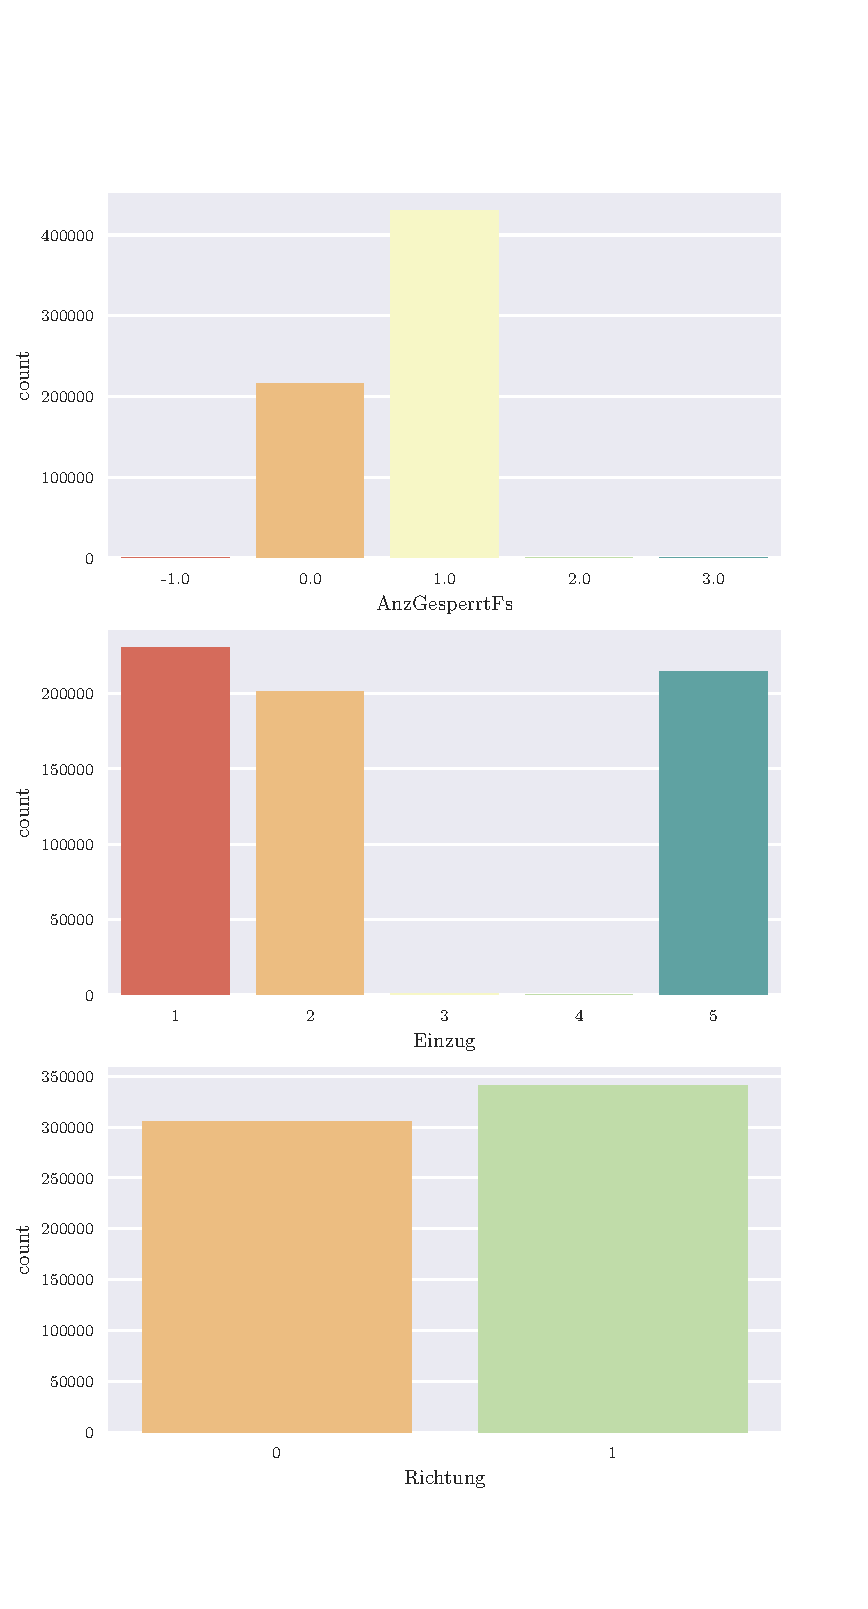
\includegraphics[scale=0.7]{CorrAnalysis/data/ArbIS/01_dataset/plots/arbis_dataset_count_multiple01}
        \caption{Distribution of the accident category \textit{AnzGesperrtFs}, \textit{Einzug} and \textit{Richtung}}
        \label{img:arbis_dataset_AnzGesperrtFs}
        \label{img:arbis_dataset_Einzug}
        \label{img:arbis_dataset_Richtung}
    \end{figure}

    \begin{figure}[ht!]
        \centering
        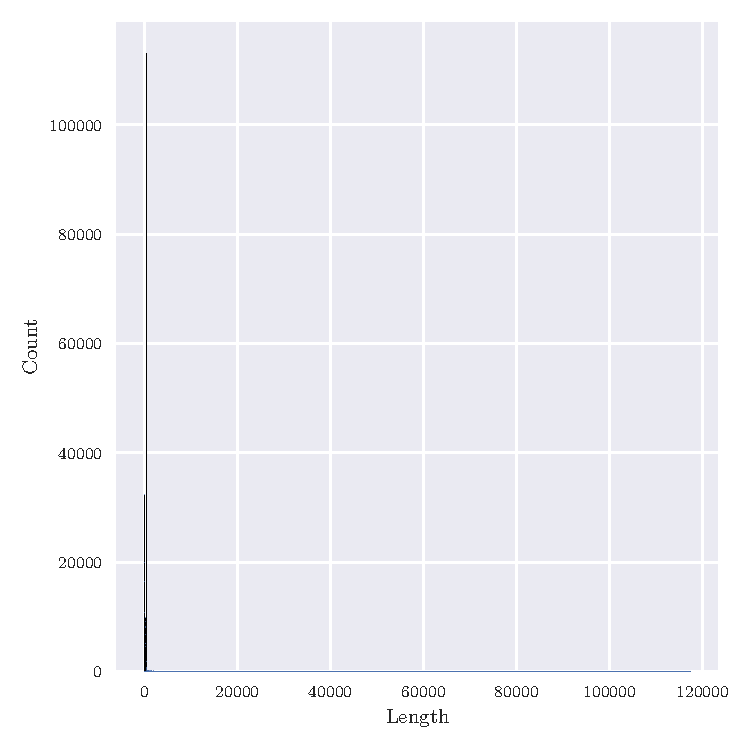
\includegraphics[scale=0.7]{CorrAnalysis/data/ArbIS/01_dataset/plots/arbis_dataset_dist_Length}
        \caption{Distribution of the roadwork parameter \textit{Length}}
        \label{img:arbis_matched_Length}
    \end{figure}

    \begin{figure}[ht!]
        \centering
        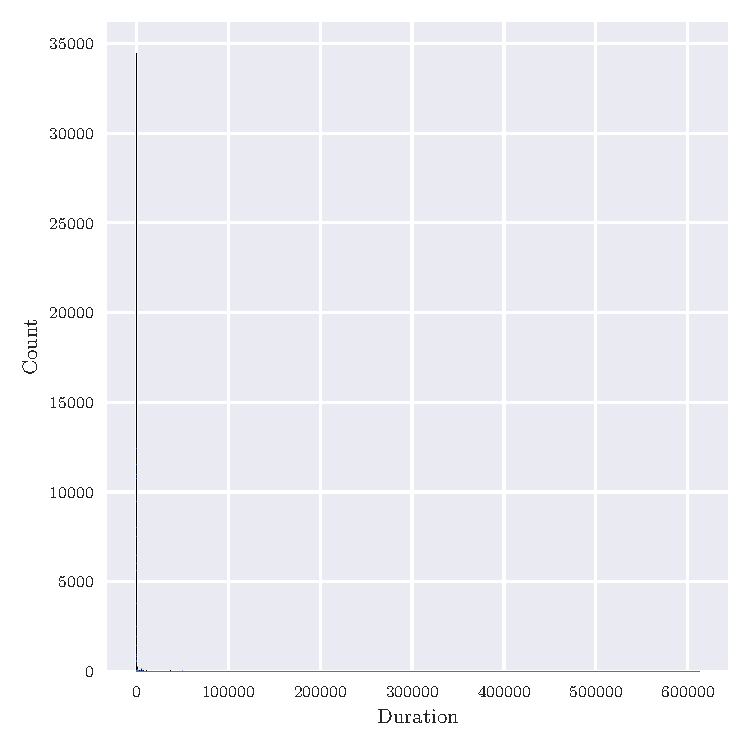
\includegraphics[scale=0.7]{CorrAnalysis/data/ArbIS/01_dataset/plots/arbis_dataset_dist_Duration}
        \caption{Distribution of the roadwork parameter \textit{Duration}}
        \label{img:arbis_matched_Duration}
    \end{figure}

    % ------- ArbIS Dataset - Tables --------
    % \newgeometry{left=1cm,right=1cm}
    \begin{table}
        \setlength{\tabcolsep}{4pt}
        \centering
        \begin{tabular}{lrrrrrrr}
\toprule
{} &  Strasse &  AnzGesperrtFs &  Einzug &  Richtung &  Length &  Duration &  Month \\
\midrule
Strasse       &     1.00 &           0.16 &    0.17 &      0.05 &    0.04 &      0.02 &   0.06 \\
AnzGesperrtFs &     0.16 &           1.00 &    0.50 &      0.00 &    0.02 &      0.11 &   0.06 \\
Einzug        &     0.17 &           0.50 &    1.00 &      0.02 &   -0.00 &     -0.15 &   0.11 \\
Richtung      &     0.05 &           0.00 &    0.02 &      1.00 &   -0.02 &     -0.00 &   0.03 \\
Length        &     0.04 &           0.02 &   -0.00 &     -0.02 &    1.00 &      0.08 &   0.04 \\
Duration      &     0.02 &           0.11 &   -0.15 &     -0.00 &    0.08 &      1.00 &   0.02 \\
Month         &     0.06 &           0.06 &    0.11 &      0.03 &    0.04 &      0.02 &   1.00 \\
\bottomrule
\end{tabular}

        \caption{Correlation matrix for ArbIS dataset, calculated with Cramer's $V$, $\eta$, $\tau$, $r_{pq}$, $r$}
        \label{tbl:appendix_arbis_correlation_matrix_dataset_cramers}
    \end{table}
    \begin{table}
        \setlength{\tabcolsep}{4pt}
        \centering
        \begin{tabular}{lrrrrrrr}
\toprule
{} &  Strasse &  AnzGesperrtFs &  Einzug &  Richtung &  Length &  Duration &  Month \\
\midrule
Strasse       &     1.00 &           0.02 &    0.03 &      0.00 &    0.04 &      0.02 &   0.01 \\
AnzGesperrtFs &     0.08 &           1.00 &    0.96 &      0.00 &    0.02 &      0.11 &   0.01 \\
Einzug        &     0.06 &           0.56 &    1.00 &      0.00 &   -0.00 &     -0.15 &   0.02 \\
Richtung      &     0.00 &           0.00 &    0.00 &      1.00 &   -0.02 &     -0.00 &   0.00 \\
Length        &     0.04 &           0.02 &   -0.00 &     -0.02 &    1.00 &      0.08 &   0.04 \\
Duration      &     0.02 &           0.11 &   -0.15 &     -0.00 &    0.08 &      1.00 &   0.02 \\
Month         &     0.01 &           0.00 &    0.01 &      0.00 &    0.04 &      0.02 &   1.00 \\
\bottomrule
\end{tabular}

        \caption{Correlation matrix for ArbIS dataset, calculated with Theil's $U$, $\eta$, $\tau$, $r_{pq}$, $r$}
        \label{tbl:appendix_arbis_correlation_matrix_dataset_theils}
    \end{table}
    \begin{table}
        \setlength{\tabcolsep}{4pt}
        \centering
        \begin{tabular}{lrrrrrrr}
\toprule
{} &  Strasse &  AnzGesperrtFs &  Einzug &  Richtung &  Length &  Duration &  Month \\
\midrule
Strasse       &      NaN &         0.0000 &  0.0000 &    0.0000 &  0.0000 &    0.0000 &    0.0 \\
AnzGesperrtFs &      0.0 &            NaN &  0.0000 &    0.2547 &  0.0000 &    0.0000 &    0.0 \\
Einzug        &      0.0 &         0.0000 &     NaN &    0.0000 &  0.0006 &    0.0000 &    0.0 \\
Richtung      &      0.0 &         0.2547 &  0.0000 &       NaN &  0.0000 &    0.0489 &    0.0 \\
Length        &      0.0 &         0.0000 &  0.0006 &    0.0000 &     NaN &    0.0000 &    0.0 \\
Duration      &      0.0 &         0.0000 &  0.0000 &    0.0489 &  0.0000 &       NaN &    0.0 \\
Month         &      0.0 &         0.0000 &  0.0000 &    0.0000 &  0.0000 &    0.0000 &    NaN \\
\bottomrule
\end{tabular}

        \caption{Significancy matrix for ArbIS dataset}
        \label{tbl:appendix_arbis_significancy_matrix_dataset}
    \end{table}
    \begin{table}
        \setlength{\tabcolsep}{4pt}
        \centering
        \begin{tabular}{llllllll}
\toprule
{} & Strasse & AnzGesperrtFs &  Einzug &  Richtung &    Length &  Duration &   Month \\
\midrule
Strasse       &     NaN &           $V$ &     $V$ &       $V$ &    $\eta$ &    $\eta$ &     $V$ \\
AnzGesperrtFs &     $V$ &           NaN &     $V$ &       $V$ &    $\tau$ &    $\tau$ &     $V$ \\
Einzug        &     $V$ &           $V$ &     NaN &       $V$ &    $\tau$ &    $\tau$ &     $V$ \\
Richtung      &     $V$ &           $V$ &     $V$ &       NaN &  $r_{pq}$ &  $r_{pq}$ &     $V$ \\
Length        &  $\eta$ &        $\tau$ &  $\tau$ &  $r_{pq}$ &       NaN &       $r$ &  $\eta$ \\
Duration      &  $\eta$ &        $\tau$ &  $\tau$ &  $r_{pq}$ &       $r$ &       NaN &  $\eta$ \\
Month         &     $V$ &           $V$ &     $V$ &       $V$ &    $\eta$ &    $\eta$ &     NaN \\
\bottomrule
\end{tabular}

        \caption{Coefficient matrix for ArbIS dataset}
        \label{tbl:appendix_arbis_coefficient_matrix_dataset}
    \end{table}
    % \restoregeometry
    
    % -------------------------------
    % ------- ArbIS Matched ---------
    % -------------------------------
    % \tocless\section{ArbIS Matched Data}
    % \label{appendix_ArbIS_matched}
    
    % ------- ArbIS Matched - Figures --------
    \begin{figure}[ht!]
        \centering
        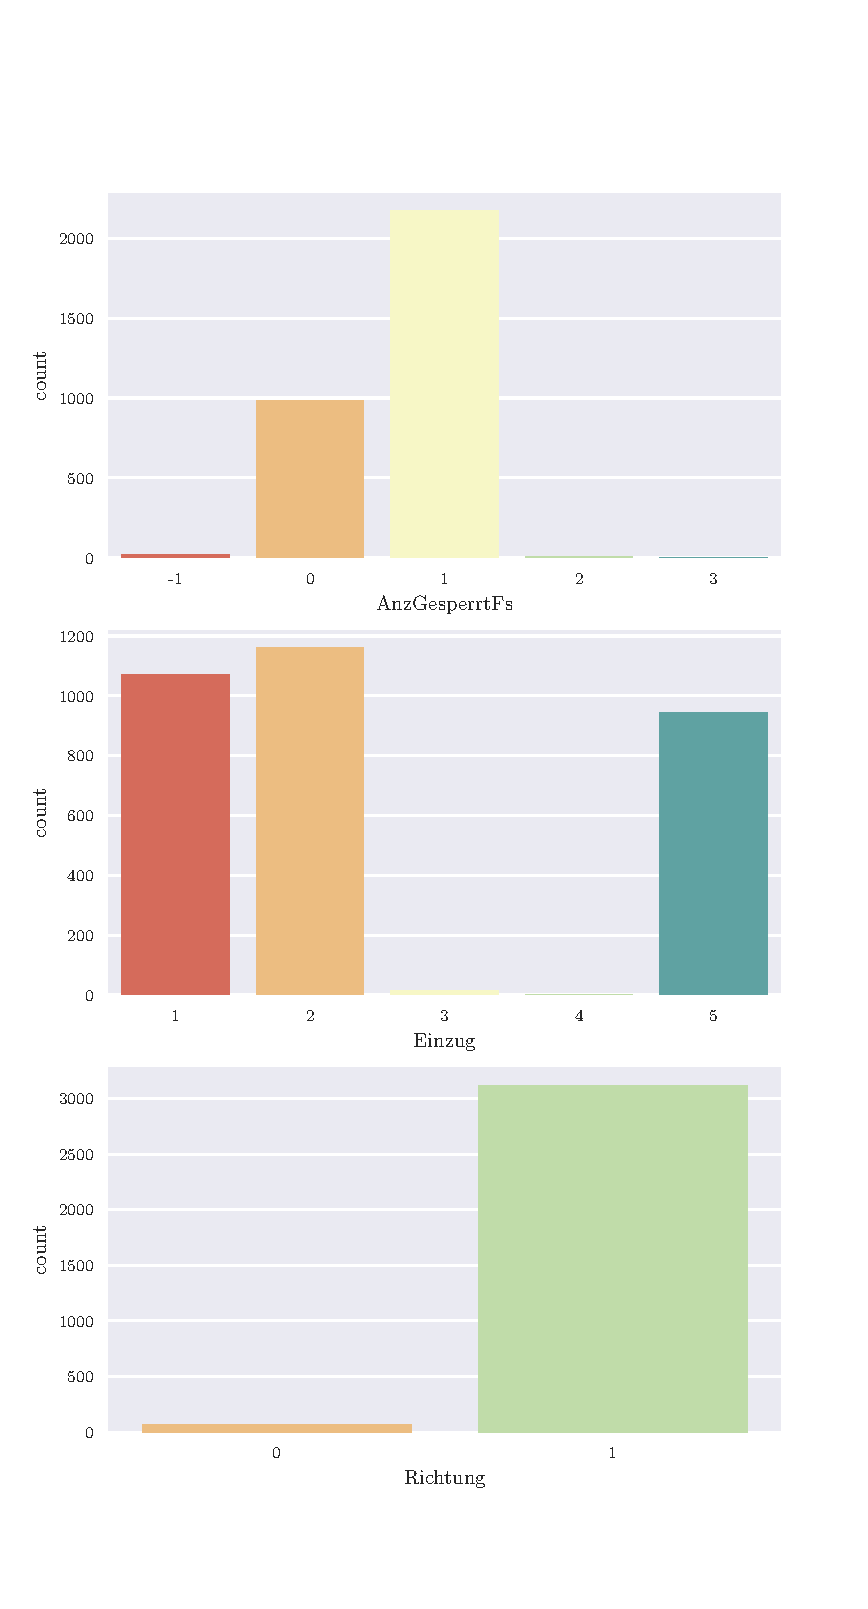
\includegraphics[scale=0.7]{CorrAnalysis/data/ArbIS/02_matched/plots/arbis_matched_count_multiple01}
        \caption{Distribution of the roadwork parameters \textit{AnzGesperrtFs}, \textit{Einzug} and \textit{Richtung}}
        \label{img:arbis_matched_AnzGesperrtFs}
        \label{img:arbis_matched_Einzug}
        \label{img:arbis_matched_Richtung}
    \end{figure}

    \begin{figure}[ht!]
        \centering
        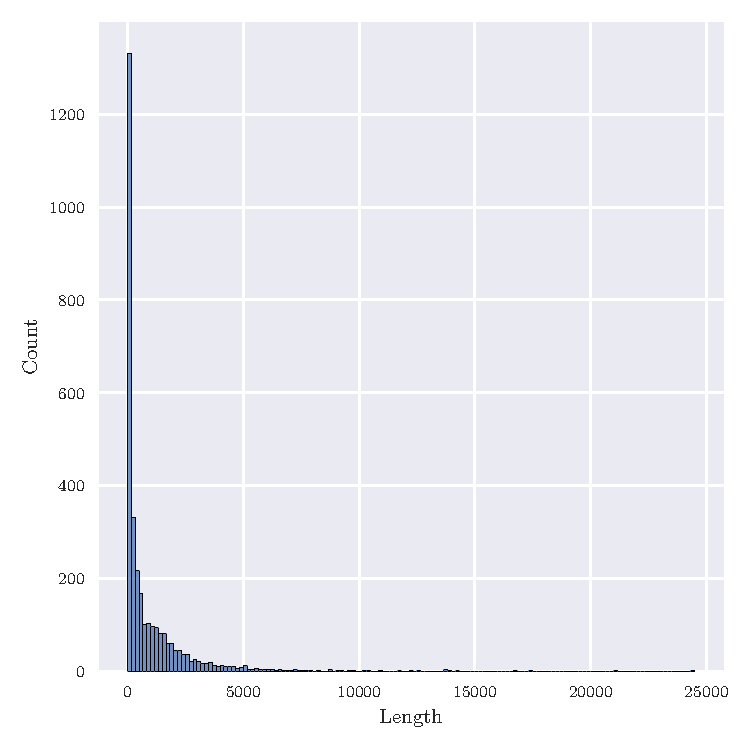
\includegraphics[scale=0.7]{CorrAnalysis/data/ArbIS/02_matched/plots/arbis_matched_dist_Length}
        \caption{Distribution of the roadwork parameter \textit{Length}}
        \label{img:arbis_matched_Length}
    \end{figure}

    \begin{figure}[ht!]
        \centering
        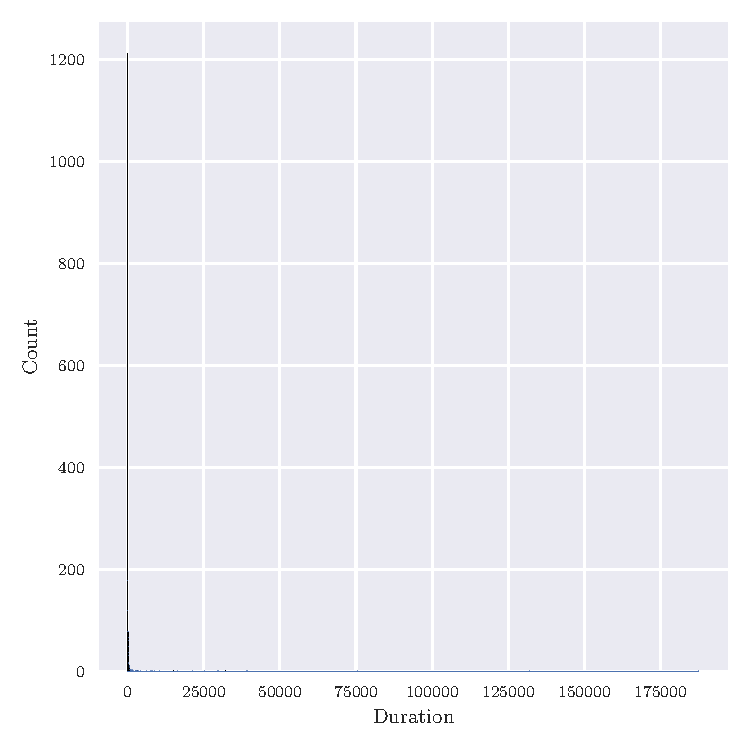
\includegraphics[scale=0.7]{CorrAnalysis/data/ArbIS/02_matched/plots/arbis_matched_dist_Duration}
        \caption{Distribution of the roadwork parameter \textit{Duration}}
        \label{img:arbis_matched_Duration}
    \end{figure}

    % ------- ArbIS Matched - Tables --------
    % \newgeometry{left=1cm,right=1cm,top=1cm}
    \begin{sidewaystable}
        \tiny
        \setlength{\tabcolsep}{4pt}
        \centering
        \begin{tabular}{lrrrrrrrrrrrrrrrr}
\toprule
{} &  TMax &  TAvg &  SMax &  SAvg &  TDist &  SDist &   Cov &  TLCar &  TLHGV &   Str &  AnzGesperrtFs &  Einzug &  Richtung &  Length &  Duration &  Month \\
\midrule
TMax          &  1.00 &  0.80 &  0.54 &  0.47 &  -0.18 &  -0.02 & -0.18 &   0.06 &   0.00 &  0.01 &          -0.04 &    0.02 &      0.02 &    0.06 &      0.02 &   0.13 \\
TAvg          &  0.80 &  1.00 &  0.24 &  0.43 &  -0.17 &  -0.00 &  0.20 &   0.04 &   0.03 & -0.01 &           0.06 &   -0.07 &      0.02 &   -0.00 &      0.02 &   0.20 \\
SMax          &  0.54 &  0.24 &  1.00 &  0.72 &  -0.14 &  -0.08 & -0.48 &   0.00 &  -0.04 & -0.04 &          -0.13 &    0.12 &     -0.01 &    0.13 &      0.00 &   0.20 \\
SAvg          &  0.47 &  0.43 &  0.72 &  1.00 &  -0.16 &  -0.11 &  0.01 &   0.00 &  -0.00 & -0.09 &          -0.06 &    0.04 &     -0.02 &    0.07 &      0.00 &   0.14 \\
TDist         & -0.18 & -0.17 & -0.14 & -0.16 &   1.00 &   0.07 & -0.02 &   0.00 &   0.02 & -0.09 &          -0.04 &    0.00 &      0.01 &   -0.06 &     -0.02 &   0.15 \\
SDist         & -0.02 & -0.00 & -0.08 & -0.11 &   0.07 &   1.00 & -0.07 &   0.01 &   0.01 & -0.03 &          -0.06 &    0.09 &      0.03 &   -0.11 &     -0.01 &   0.13 \\
Cov           & -0.18 &  0.20 & -0.48 &  0.01 &  -0.02 &  -0.07 &  1.00 &  -0.07 &  -0.03 &  0.08 &           0.17 &   -0.16 &     -0.00 &   -0.11 &     -0.01 &   0.22 \\
TLCar         &  0.06 &  0.04 &  0.00 &  0.00 &   0.00 &   0.01 & -0.07 &   1.00 &   0.10 & -0.07 &          -0.03 &    0.01 &     -0.02 &    0.02 &      0.00 &   0.14 \\
TLHGV         &  0.00 &  0.03 & -0.04 & -0.00 &   0.02 &   0.01 & -0.03 &   0.10 &   1.00 & -0.08 &          -0.02 &    0.01 &      0.03 &    0.00 &      0.02 &   0.12 \\
Str           &  0.01 & -0.01 & -0.04 & -0.09 &  -0.09 &  -0.03 &  0.08 &  -0.07 &  -0.08 &  1.00 &          -0.02 &    0.05 &     -0.02 &   -0.04 &     -0.02 &   0.27 \\
AnzGesperrtFs & -0.04 &  0.06 & -0.13 & -0.06 &  -0.04 &  -0.06 &  0.17 &  -0.03 &  -0.02 & -0.02 &           1.00 &    0.50 &      0.18 &   -0.02 &      0.14 &   0.10 \\
Einzug        &  0.02 & -0.07 &  0.12 &  0.04 &   0.00 &   0.09 & -0.16 &   0.01 &   0.01 &  0.05 &           0.50 &    1.00 &      0.14 &    0.03 &     -0.13 &   0.14 \\
Richtung      &  0.02 &  0.02 & -0.01 & -0.02 &   0.01 &   0.03 & -0.00 &  -0.02 &   0.03 & -0.02 &           0.18 &    0.14 &      1.00 &   -0.05 &     -0.07 &   0.14 \\
Length        &  0.06 & -0.00 &  0.13 &  0.07 &  -0.06 &  -0.11 & -0.11 &   0.02 &   0.00 & -0.04 &          -0.02 &    0.03 &     -0.05 &    1.00 &      0.07 &   0.09 \\
Duration      &  0.02 &  0.02 &  0.00 &  0.00 &  -0.02 &  -0.01 & -0.01 &   0.00 &   0.02 & -0.02 &           0.14 &   -0.13 &     -0.07 &    0.07 &      1.00 &   0.05 \\
Month         &  0.13 &  0.20 &  0.20 &  0.14 &   0.15 &   0.13 &  0.22 &   0.14 &   0.12 &  0.27 &           0.10 &    0.14 &      0.14 &    0.09 &      0.05 &   1.00 \\
\bottomrule
\end{tabular}

        \caption{Correlation matrix for ArbIS matched data, calculated with Cramer's $V$, $\eta$, $\tau$, $r_{pq}$, $r$}
    \end{sidewaystable}
    \begin{sidewaystable}
        \tiny
        \setlength{\tabcolsep}{4pt}
        \centering
        \begin{tabular}{lrrrrrrrrrrrrrrrr}
\toprule
{} &  TMax &  TAvg &  SMax &  SAvg &  TDist &  SDist &   Cov &  TLCar &  TLHGV &   Str &  AnzGesperrtFs &  Einzug &  Richtung &  Length &  Duration &  Month \\
\midrule
TMax          &  1.00 &  0.80 &  0.54 &  0.47 &  -0.18 &  -0.02 & -0.18 &   0.06 &   0.00 &  0.01 &          -0.04 &    0.02 &      0.02 &    0.06 &      0.02 &   0.13 \\
TAvg          &  0.80 &  1.00 &  0.24 &  0.43 &  -0.17 &  -0.00 &  0.20 &   0.04 &   0.03 & -0.01 &           0.06 &   -0.07 &      0.02 &   -0.00 &      0.02 &   0.20 \\
SMax          &  0.54 &  0.24 &  1.00 &  0.72 &  -0.14 &  -0.08 & -0.48 &   0.00 &  -0.04 & -0.04 &          -0.13 &    0.12 &     -0.01 &    0.13 &      0.00 &   0.20 \\
SAvg          &  0.47 &  0.43 &  0.72 &  1.00 &  -0.16 &  -0.11 &  0.01 &   0.00 &  -0.00 & -0.09 &          -0.06 &    0.04 &     -0.02 &    0.07 &      0.00 &   0.14 \\
TDist         & -0.18 & -0.17 & -0.14 & -0.16 &   1.00 &   0.07 & -0.02 &   0.00 &   0.02 & -0.09 &          -0.04 &    0.00 &      0.01 &   -0.06 &     -0.02 &   0.15 \\
SDist         & -0.02 & -0.00 & -0.08 & -0.11 &   0.07 &   1.00 & -0.07 &   0.01 &   0.01 & -0.03 &          -0.06 &    0.09 &      0.03 &   -0.11 &     -0.01 &   0.13 \\
Cov           & -0.18 &  0.20 & -0.48 &  0.01 &  -0.02 &  -0.07 &  1.00 &  -0.07 &  -0.03 &  0.08 &           0.17 &   -0.16 &     -0.00 &   -0.11 &     -0.01 &   0.22 \\
TLCar         &  0.06 &  0.04 &  0.00 &  0.00 &   0.00 &   0.01 & -0.07 &   1.00 &   0.10 & -0.07 &          -0.03 &    0.01 &     -0.02 &    0.02 &      0.00 &   0.14 \\
TLHGV         &  0.00 &  0.03 & -0.04 & -0.00 &   0.02 &   0.01 & -0.03 &   0.10 &   1.00 & -0.08 &          -0.02 &    0.01 &      0.03 &    0.00 &      0.02 &   0.12 \\
Str           &  0.01 & -0.01 & -0.04 & -0.09 &  -0.09 &  -0.03 &  0.08 &  -0.07 &  -0.08 &  1.00 &          -0.02 &    0.05 &     -0.02 &   -0.04 &     -0.02 &   0.27 \\
AnzGesperrtFs & -0.04 &  0.06 & -0.13 & -0.06 &  -0.04 &  -0.06 &  0.17 &  -0.03 &  -0.02 & -0.02 &           1.00 &    0.83 &      0.01 &   -0.02 &      0.14 &   0.03 \\
Einzug        &  0.02 & -0.07 &  0.12 &  0.04 &   0.00 &   0.09 & -0.16 &   0.01 &   0.01 &  0.05 &           0.50 &    1.00 &      0.00 &    0.03 &     -0.13 &   0.03 \\
Richtung      &  0.02 &  0.02 & -0.01 & -0.02 &   0.01 &   0.03 & -0.00 &  -0.02 &   0.03 & -0.02 &           0.05 &    0.03 &      1.00 &   -0.05 &     -0.07 &   0.06 \\
Length        &  0.06 & -0.00 &  0.13 &  0.07 &  -0.06 &  -0.11 & -0.11 &   0.02 &   0.00 & -0.04 &          -0.02 &    0.03 &     -0.05 &    1.00 &      0.07 &   0.09 \\
Duration      &  0.02 &  0.02 &  0.00 &  0.00 &  -0.02 &  -0.01 & -0.01 &   0.00 &   0.02 & -0.02 &           0.14 &   -0.13 &     -0.07 &    0.07 &      1.00 &   0.05 \\
Month         &  0.13 &  0.20 &  0.20 &  0.14 &   0.15 &   0.13 &  0.22 &   0.14 &   0.12 &  0.27 &           0.01 &    0.02 &      0.00 &    0.09 &      0.05 &   1.00 \\
\bottomrule
\end{tabular}

        \caption{Correlation matrix for ArbIS matched data, calculated with Theil's $U$, $\eta$, $\tau$, $r_{pq}$, $r$}
    \end{sidewaystable}
    \begin{sidewaystable}
        \tiny
        \setlength{\tabcolsep}{4pt}
        \centering
        \begin{tabular}{lrrrrrrrrrrrrrrrr}
\toprule
{} &  TMax &  TAvg &  SMax &  SAvg &  TDist &  SDist &   Cov &  TLCar &  TLHGV &   Str &   AGF &  Einzug &  Richtung &  Length &  Duration &  Month \\
\midrule
TMax     &   nan & 0.000 & 0.000 & 0.000 &  0.000 &  0.385 & 0.000 &  0.001 &  0.965 & 0.000 & 0.024 &   0.107 &     0.267 &   0.001 &     0.173 &  0.000 \\
TAvg     & 0.000 &   nan & 0.000 & 0.000 &  0.000 &  0.953 & 0.000 &  0.047 &  0.071 & 0.000 & 0.011 &   0.000 &     0.301 &   0.987 &     0.340 &  0.000 \\
SMax     & 0.000 & 0.000 &   nan & 0.000 &  0.000 &  0.000 & 0.000 &  0.859 &  0.034 & 0.000 & 0.000 &   0.000 &     0.451 &   0.000 &     0.993 &  0.000 \\
SAvg     & 0.000 & 0.000 & 0.000 &   nan &  0.000 &  0.000 & 0.663 &  0.988 &  0.896 & 0.000 & 0.041 &   0.004 &     0.397 &   0.000 &     0.934 &  0.000 \\
TDist    & 0.000 & 0.000 & 0.000 & 0.000 &    nan &  0.000 & 0.201 &  0.819 &  0.190 & 0.000 & 0.452 &   0.765 &     0.506 &   0.001 &     0.163 &  0.000 \\
SDist    & 0.385 & 0.953 & 0.000 & 0.000 &  0.000 &    nan & 0.000 &  0.527 &  0.445 & 0.000 & 0.000 &   0.000 &     0.063 &   0.000 &     0.433 &  0.000 \\
Cov      & 0.000 & 0.000 & 0.000 & 0.663 &  0.201 &  0.000 &   nan &  0.000 &  0.050 & 0.000 & 0.000 &   0.000 &     0.799 &   0.000 &     0.508 &  0.000 \\
TLCar    & 0.001 & 0.047 & 0.859 & 0.988 &  0.819 &  0.527 & 0.000 &    nan &  0.000 & 0.000 & 0.032 &   0.350 &     0.229 &   0.183 &     0.913 &  0.000 \\
TLHGV    & 0.965 & 0.071 & 0.034 & 0.896 &  0.190 &  0.445 & 0.050 &  0.000 &    nan & 0.000 & 0.237 &   0.677 &     0.112 &   0.802 &     0.279 &  0.000 \\
Str      & 0.000 & 0.000 & 0.000 & 0.000 &  0.000 &  0.000 & 0.000 &  0.000 &  0.000 &   nan & 0.000 &   0.000 &     0.000 &   0.000 &     0.000 &  0.000 \\
AGF      & 0.024 & 0.011 & 0.000 & 0.041 &  0.452 &  0.000 & 0.000 &  0.032 &  0.237 & 0.000 &   nan &   0.000 &     0.000 &   0.002 &     0.000 &  0.000 \\
Einzug   & 0.107 & 0.000 & 0.000 & 0.004 &  0.765 &  0.000 & 0.000 &  0.350 &  0.677 & 0.000 & 0.000 &     nan &     0.000 &   0.046 &     0.000 &  0.000 \\
Richtung & 0.267 & 0.301 & 0.451 & 0.397 &  0.506 &  0.063 & 0.799 &  0.229 &  0.112 & 0.000 & 0.000 &   0.000 &       nan &   0.008 &     0.000 &  0.000 \\
Length   & 0.001 & 0.987 & 0.000 & 0.000 &  0.001 &  0.000 & 0.000 &  0.183 &  0.802 & 0.000 & 0.002 &   0.046 &     0.008 &     nan &     0.000 &  0.000 \\
Duration & 0.173 & 0.340 & 0.993 & 0.934 &  0.163 &  0.433 & 0.508 &  0.913 &  0.279 & 0.000 & 0.000 &   0.000 &     0.000 &   0.000 &       nan &  0.000 \\
Month    & 0.000 & 0.000 & 0.000 & 0.000 &  0.000 &  0.000 & 0.000 &  0.000 &  0.000 & 0.000 & 0.000 &   0.000 &     0.000 &   0.000 &     0.000 &    nan \\
\bottomrule
\end{tabular}

        \caption{Significancy matrix for ArbIS matched data}
    \end{sidewaystable}
    \begin{sidewaystable}
        \tiny
        \setlength{\tabcolsep}{4pt}
        \centering
        \begin{tabular}{lllllllllllllllll}
\toprule
{} &      TMax &      TAvg &      SMax &      SAvg &     TDist &     SDist &       Cov &     TLCar &     TLHGV &       Str & AnzGesperrtFs &  Einzug &  Richtung &    Length &  Duration &   Month \\
\midrule
TMax          &       NaN &       $r$ &       $r$ &       $r$ &       $r$ &       $r$ &       $r$ &       $r$ &       $r$ &       $r$ &        $\tau$ &  $\tau$ &  $r_{pq}$ &       $r$ &       $r$ &  $\eta$ \\
TAvg          &       $r$ &       NaN &       $r$ &       $r$ &       $r$ &       $r$ &       $r$ &       $r$ &       $r$ &       $r$ &        $\tau$ &  $\tau$ &  $r_{pq}$ &       $r$ &       $r$ &  $\eta$ \\
SMax          &       $r$ &       $r$ &       NaN &       $r$ &       $r$ &       $r$ &       $r$ &       $r$ &       $r$ &       $r$ &        $\tau$ &  $\tau$ &  $r_{pq}$ &       $r$ &       $r$ &  $\eta$ \\
SAvg          &       $r$ &       $r$ &       $r$ &       NaN &       $r$ &       $r$ &       $r$ &       $r$ &       $r$ &       $r$ &        $\tau$ &  $\tau$ &  $r_{pq}$ &       $r$ &       $r$ &  $\eta$ \\
TDist         &       $r$ &       $r$ &       $r$ &       $r$ &       NaN &       $r$ &       $r$ &       $r$ &       $r$ &       $r$ &        $\tau$ &  $\tau$ &  $r_{pq}$ &       $r$ &       $r$ &  $\eta$ \\
SDist         &       $r$ &       $r$ &       $r$ &       $r$ &       $r$ &       NaN &       $r$ &       $r$ &       $r$ &       $r$ &        $\tau$ &  $\tau$ &  $r_{pq}$ &       $r$ &       $r$ &  $\eta$ \\
Cov           &       $r$ &       $r$ &       $r$ &       $r$ &       $r$ &       $r$ &       NaN &       $r$ &       $r$ &       $r$ &        $\tau$ &  $\tau$ &  $r_{pq}$ &       $r$ &       $r$ &  $\eta$ \\
TLCar         &       $r$ &       $r$ &       $r$ &       $r$ &       $r$ &       $r$ &       $r$ &       NaN &       $r$ &       $r$ &        $\tau$ &  $\tau$ &  $r_{pq}$ &       $r$ &       $r$ &  $\eta$ \\
TLHGV         &       $r$ &       $r$ &       $r$ &       $r$ &       $r$ &       $r$ &       $r$ &       $r$ &       NaN &       $r$ &        $\tau$ &  $\tau$ &  $r_{pq}$ &       $r$ &       $r$ &  $\eta$ \\
Str           &       $r$ &       $r$ &       $r$ &       $r$ &       $r$ &       $r$ &       $r$ &       $r$ &       $r$ &       NaN &        $\tau$ &  $\tau$ &  $r_{pq}$ &       $r$ &       $r$ &  $\eta$ \\
AnzGesperrtFs &    $\tau$ &    $\tau$ &    $\tau$ &    $\tau$ &    $\tau$ &    $\tau$ &    $\tau$ &    $\tau$ &    $\tau$ &    $\tau$ &           NaN &     $V$ &       $V$ &    $\tau$ &    $\tau$ &     $V$ \\
Einzug        &    $\tau$ &    $\tau$ &    $\tau$ &    $\tau$ &    $\tau$ &    $\tau$ &    $\tau$ &    $\tau$ &    $\tau$ &    $\tau$ &           $V$ &     NaN &       $V$ &    $\tau$ &    $\tau$ &     $V$ \\
Richtung      &  $r_{pq}$ &  $r_{pq}$ &  $r_{pq}$ &  $r_{pq}$ &  $r_{pq}$ &  $r_{pq}$ &  $r_{pq}$ &  $r_{pq}$ &  $r_{pq}$ &  $r_{pq}$ &           $V$ &     $V$ &       NaN &  $r_{pq}$ &  $r_{pq}$ &     $V$ \\
Length        &       $r$ &       $r$ &       $r$ &       $r$ &       $r$ &       $r$ &       $r$ &       $r$ &       $r$ &       $r$ &        $\tau$ &  $\tau$ &  $r_{pq}$ &       NaN &       $r$ &  $\eta$ \\
Duration      &       $r$ &       $r$ &       $r$ &       $r$ &       $r$ &       $r$ &       $r$ &       $r$ &       $r$ &       $r$ &        $\tau$ &  $\tau$ &  $r_{pq}$ &       $r$ &       NaN &  $\eta$ \\
Month         &    $\eta$ &    $\eta$ &    $\eta$ &    $\eta$ &    $\eta$ &    $\eta$ &    $\eta$ &    $\eta$ &    $\eta$ &    $\eta$ &           $V$ &     $V$ &       $V$ &    $\eta$ &    $\eta$ &     NaN \\
\bottomrule
\end{tabular}

        \caption{Coefficient matrix for ArbIS matched data}
    \end{sidewaystable}
    % \restoregeometry

\end{appendices}
    
